%----------------------------------------------------------------------------------------
%	PACKAGES AND OTHER DOCUMENT CONFIGURATIONS
%----------------------------------------------------------------------------------------

%----------------------------------------------------------------------------------------
%		Géometrie de la page
%----------------------------------------------------------------------------------------
\documentclass[dvipsnames,french,10pt]{book}

\usepackage[
paperheight=24cm, %hauteur du papier
paperwidth=18cm, %largeur du papier
left=1cm, %marge de gauche
right=1cm, %marge de droite
top=1.5cm, %marge du haut
bottom=1.6cm, %marge du bas
%marginparsep=0pt, %distance entre le texte et les notes de marges 
reversemp, %inverse l'emplacement de la marge
headheight=20.60pt %hauteur du header
%showframe, %permet d'afficher le cadre défini ci-dessus
%bindingoffset=1cm %permet d'ajouter le décalage dû au reliage
]{geometry} %Redéfinition de la taille des pages
\raggedbottom


%----------------------------------------------------------------------------------------
%		Generals
%----------------------------------------------------------------------------------------
%\usepackage{fourier} %!! A changer plus tard !!
\usepackage[scaled]{uarial}
\renewcommand*\familydefault{\sfdefault} %% Only if the base font of the document is to be sans serif
\usepackage{frcursive}
\usepackage[T1]{fontenc} %Accents handling
\usepackage[utf8]{inputenc} % Use UTF-8 encoding
%\usepackage{microtype} % Slightly tweak font spacing for aesthetics
\usepackage[english, francais]{babel} % Language hyphenation and typographical rules
\usepackage{marginnote}

%----------------------------------------------------------------------------------------
%		Graphics
%----------------------------------------------------------------------------------------
\usepackage{xcolor}
\usepackage{graphicx, multicol} % Enhanced support for graphics
\graphicspath{{FIG/}{FIG/NetC_fractions_decimales/}{FIG/NetC_fractions/}{FIG/NetC_les_nombres_entiers/}{FIG/NetC_nombres_decimaux}}
\usepackage{wrapfig}
\usepackage{colortbl}

%\usepackage{xsavebox}
% Il faudrait utiliser xsavebox à l'avenir pour réduire la taille du pdf

%----------------------------------------------------------------------------------------
%		Other packages
%----------------------------------------------------------------------------------------
\usepackage{hyperref}
\hypersetup{
	colorlinks=true, %colorise les liens
	breaklinks=true, %permet le retour à la ligne dans les liens trop longs
	urlcolor= sacado_violet,  %couleur des hyperliens et des QR codes
	linkcolor= sacado_violet, %couleur des liens internes
	plainpages=false  %pour palier à "Bookmark problems can occur when you have duplicate page numbers, for example, if you have a page i and a page 1."
}
\usepackage{tabularx}
\newcolumntype{M}[1]{>{\arraybackslash}m{#1}} %Defines a scalable column type in tabular
\usepackage{booktabs} % Enhances quality of tables
\usepackage{diagbox} % barre en diagonale dans un tableau
\usepackage{multicol}
\usepackage[explicit]{titlesec}
\usepackage{xr}
\usepackage{xspace}
\usepackage{array}
\usepackage{listings}
\usepackage{fancyvrb} %verbatim
\usepackage{stmaryrd}
\usepackage{float}


%----------------------------------------------------------------------------------------
%		Headers and footers
%----------------------------------------------------------------------------------------

\pagestyle{empty}
\usepackage{fancyhdr}
\pagestyle{fancy}
\renewcommand{\headrulewidth}{0pt} % pas de filet sous le header

%----------------------------------------------------------------------------------------
%		Mathematics packages
%----------------------------------------------------------------------------------------
\usepackage{amsthm, amsmath, amssymb, mathrsfs} % Mathematical typesetting
\usepackage{marvosym, wasysym} % More symbols
\usepackage[makeroom]{cancel}
\usepackage{xlop}
\usepackage{pgf,tikz,pgfplots}
\pgfplotsset{compat=1.16}
\usepackage{pgf-pie}
\usetikzlibrary{positioning}
\usetikzlibrary{arrows}
\usepackage{pst-plot,pst-tree,pst-func, pstricks-add,pst-node,pst-text}
%\usepackage{units}
\usepackage{nicefrac}
\usepackage[np]{numprint} %Séparation milliers dans un nombre \np{12345} donne 12 345
\usepackage{multido}
\newcommand{\RNum}[1]{\uppercase\expandafter{\romannumeral #1\relax}}

%----------------------------------------------------------------------------------------
%		New text commands
%----------------------------------------------------------------------------------------
\usepackage{calc}
\usepackage{boites}
 \renewcommand{\arraystretch}{1.6}

%%%%% Pour les imports.
\usepackage{import}

%%%%% Pour faire des boites
\usepackage[tikz]{bclogo}
\usepackage{bclogo}
\usepackage{framed}
\usepackage[skins]{tcolorbox}
\tcbuselibrary{breakable}
\tcbuselibrary{skins}
\usetikzlibrary{quotes,babel,arrows.meta,shadows,decorations.pathmorphing,decorations.markings,patterns}
\usepackage{tikzpagenodes}
\usetikzlibrary{plotmarks}

%%%%% Pour les symboles et les ensembles
%\newcommand{\pp}{\leq}
%\newcommand{\pg}{\geq}
%%\newcommand{\euro}{\eurologo{}}
%\newcommand{\R}{\mathbb{R}}
%\newcommand{\N}{\mathbb{N}}
%\newcommand{\D}{\mathbb{D}}
%\newcommand{\Z}{\mathbb{Z}}
%\newcommand{\Q}{\mathbb{Q}}
%\newcommand{\C}{\mathbb{C}}

%%%%% Pour une double minipage
\newcommand{\mini}[4]{
\begin{minipage}[c]{#1}
#2
\end{minipage}
\hfill
\begin{minipage}[c]{#3}
#4
\end{minipage}
}


%\newcommand\hole[1]{\texttt{\_}}
%\newcommand{\PROP}[1]{\textbf{\underline{#1}}}
%\newcommand{\exercice}{\textcolor{OliveGreen}{Exercice : }}
%\newcommand{\correction}{\textcolor{BurntOrange}{Correction : }}
%\newcommand{\propriete}{\textbf{\underline{Propriété}} : }
%\newcommand{\prop}{\textbf{\underline{Propriété}} : }
%\newcommand{\vocabulaire}{\textbf{\underline{Vocabulaire}} : }
%\newcommand{\voca}{\textbf{\underline{Vocabulaire}} : }

\usepackage{enumitem}
\newlist{todolist}{itemize}{2} %Pour faire des QCM
\setlist[todolist]{label=$\square$} %Pour faire des QCM \begin{todolist} instead of itemize
\renewcommand{\FrenchLabelItem}{\textbullet} %bullet dans les items


%----------------------------------------------------------------------------------------
%		Définition de couleurs pour ...
%----------------------------------------------------------------------------------------

%GEOGEBRA

\definecolor{zzttqq}{rgb}{0.6,0.2,0.} %rouge des polygones
\definecolor{qqqqff}{rgb}{0.,0.,1.}
\definecolor{xdxdff}{rgb}{0.49019607843137253,0.49019607843137253,1.}%bleu
\definecolor{qqwuqq}{rgb}{0.,0.39215686274509803,0.} %vert des angles
\definecolor{ffqqqq}{rgb}{1.,0.,0.} %rouge vif
\definecolor{uuuuuu}{rgb}{0.26666666666666666,0.26666666666666666,0.26666666666666666}
\definecolor{qqzzqq}{rgb}{0.,0.6,0.}
\definecolor{cqcqcq}{rgb}{0.7529411764705882,0.7529411764705882,0.7529411764705882} %gris
\definecolor{qqffqq}{rgb}{0.,1.,0.}
\definecolor{ffdxqq}{rgb}{1.,0.8431372549019608,0.}
\definecolor{ffffff}{rgb}{1.,1.,1.}
\definecolor{ududff}{rgb}{0.30196078431372547,0.30196078431372547,1.}
\definecolor{ffqqff}{rgb}{1.,0.,1.}
\definecolor{ffxfqq}{rgb}{1,0.4980392156862745,0}
\definecolor{ffffqq}{rgb}{1,1,0}
\definecolor{qqttzz}{rgb}{0,0.2,0.6}
\definecolor{qqccqq}{rgb}{0,0.8,0}
\definecolor{qqzzff}{rgb}{0,0.6,1}
\definecolor{qqwwzz}{rgb}{0,0.4,0.6}
\definecolor{eqeqeq}{rgb}{0.8784313725490196,0.8784313725490196,0.8784313725490196}

%SACADO

\definecolor{fond}{HTML}{6818A2}  %couleur des entetes etc.  violet sacado
\definecolor{sacado_purple}{RGB}{94,68,145} %% Violet foncé Sacado
\definecolor{sacado_violet}{RGB}{153,117,224} %% Violet clair Sacado
\definecolor{texte}{HTML}{FFFFFF} % couleur du texte des entetes etc.
\definecolor{sacado_blue}{RGB}{0,129,159} %% Bleu Sacado
\definecolor{sacado_green}{RGB}{59, 157, 38} %% Vert Sacado
\definecolor{sacado_yellow}{RGB}{255,180,0} %% Jaune Sacado
\definecolor{sacado_purple}{RGB}{94,68,145} %% Violet foncé Sacado
\definecolor{sacado_violet}{RGB}{153,117,224} %% Violet clair Sacado
\definecolor{sacado_orange}{HTML}{FF8B69} %% Orange Sacado
\definecolor{sacado_red}{HTML}{A11915} %% Rouge Sacado
\definecolor{sacado_gray}{HTML}{7B7485} %% Gris Sacado
%BOITES 

\definecolor{bleu1}{rgb}{0.54,0.79,0.95} %% Bleu
\definecolor{sapgreen}{rgb}{0.4, 0.49, 0}
\definecolor{dvzfxr}{rgb}{0.7,0.4,0.}
\definecolor{beamer}{rgb}{0.5176470588235295,0.49019607843137253,0.32941176470588235} % couleur beamer
\definecolor{preuveRbeamer}{rgb}{0.8,0.4,0}
\definecolor{sectioncolor}{rgb}{0.24,0.21,0.44}
\definecolor{subsectioncolor}{rgb}{0.1,0.21,0.61}
\definecolor{subsubsectioncolor}{rgb}{0.1,0.21,0.61}
\definecolor{info}{rgb}{0.82,0.62,0}
\definecolor{bleu2}{rgb}{0.38,0.56,0.68}
\definecolor{bleu3}{rgb}{0.24,0.34,0.40}
\definecolor{bleu4}{rgb}{0.12,0.20,0.25}
\definecolor{vert}{rgb}{0.21,0.33,0}
\definecolor{vertS}{rgb}{0.05,0.6,0.42}
\definecolor{red}{rgb}{0.78,0,0}
\definecolor{color5}{rgb}{0,0.4,0.58}
\definecolor{eduscol4B}{rgb}{0.19,0.53,0.64}
\definecolor{eduscol4P}{rgb}{0.62,0.12,0.39}
\definecolor{ill_frame}{HTML}{F0F0F0} %Boite illustration contour
\definecolor{ill_back}{HTML}{F7F7F7}  %Boite illustration background
\definecolor{ill_title}{HTML}{AAAAAA} %Boite illustration titre

%----------------------------------------------------------------------------------------
%		QR codes
%----------------------------------------------------------------------------------------

\usepackage[
%final %Pour la compilation finale
draft %Pour le travail sur les documents
]{qrcode}
\usepackage{fontawesome}
\usepackage{fancyqr}
\FancyQrLoad{flat}
\fancyqrset{
%image=\scalebox{.8}{
\includegraphics[scale=1]{sacadoA1.png}},image padding=.5,
l color=sacado_violet,r color=sacado_blue}
\newcommand{\qr}[2]{\centering \fancyqr{https://sacado.xyz/qcm/show_course_from_qrcode/#1}

\vspace{.2cm}

#2} %\qr{id} Pour obtenir un qrcode en indiquant seulement l'id de l'exercice





\newcommand{\miniqr}[3]{
\begin{minipage}[c]{.8\linewidth}
#1
\end{minipage}
\hfill
\fbox{
\begin{minipage}[c]{.18\linewidth}
\begin{center}
\fancyqr{https://sacado.xyz/qcm/show\_course\_from\_qrcode/#2}

\vspace{.2cm}

#3
\end{center}
\end{minipage}
}
}



%practice/frombook/<int:ide>/ pour accéder à un exercice depuis le livre.
%----------------------------------------
%
%   Définitions des environnements "pageCours" et "pageExos"
%
%----------------------------------------

\newcounter{cpt}
\newcounter{exo}
\newcounter{cptr}

\newcommand{\titreChap}{Titre de chapitre à définir}

\renewcommand{\chapter}[3]{
  \stepcounter{chapter}
  \setcounter{exo}{0}
  \setcounter{cpt}{0}
  
%\cleardoublepage  % pour commencer à droite
{\Huge \hfill Chapitre \Roman{chapter}.\\
  \bigskip
  #1\\
  \bigskip {\begin{center}
  \fancyqr[image={
\includegraphics[scale=.6]{sacadoA1.png}},image padding=.5,height=5cm]{#2}
  \end{center}}  {\normalsize #3}}
\renewcommand{\titreChap}{#1}

%\ifthenelse{\equal{#2}{}}{}{\par
%  \bigskip\bigskip
%  #2}
\newpage
}

\renewenvironment{leftbar}[1][\hsize]
{%
    \def\FrameCommand
    {%
        {\color{black}\vrule width 0.5pt}%
        \hspace{4pt}%must no space.
        \fboxsep=\FrameSep%\colorbox{yellow}%
    }%
    \MakeFramed{\hsize#1\advance\hsize-\width\FrameRestore}%
}
{\endMakeFramed}


\newcommand{\headerGeneral}[3]{ % intitulé, couleur, qrcode
\begin{tikzpicture}[remember picture,overlay]
\coordinate(NO) at (-2,0);
\coordinate(SW) at (22,1);
\coordinate(titre) at (0,0.2);
%\coordinate(qr) at (16.85,0.);
\shade[left color=#2 , right color=#2 ] (NO) rectangle (SW);
\draw (titre) node[color=texte, anchor=west]{ {\large \bf  #1} \quad\quad \bf {\small \titreChap} };
%\draw (qr) node {\qr{#3}};
\end{tikzpicture}
}

\newenvironment{pageCours}{\lhead{%
\pagecolor{white!100}
\headerGeneral{COURS}{fond!70}{p/1234}
}\begin{leftbar}}{\end{leftbar}\newpage}

\newenvironment{pageAD}{\lhead{%
\pagecolor{sacado_violet!6}
\headerGeneral{APPLICATIONS DIRECTES}{sacado_violet!70}{p/1234}
} }{ \newpage}

\newenvironment{pageParcoursu}{\lhead{%
\pagecolor{sacado_green!6} 
\headerGeneral{PARCOURS 1}{sacado_green}{p/1234}
} }{ \newpage}


\newenvironment{pageParcoursd}{\lhead{%
\pagecolor{sacado_blue!6}
\headerGeneral{PARCOURS 2}{sacado_blue_light}{p/1234}
} }{ \newpage}

\newenvironment{pageParcourst}{\lhead{%
\pagecolor{sacado_red!6}
\headerGeneral{PARCOURS 3}{sacado_red}{p/1234}
} }{ \newpage}

\newenvironment{pageBrouillon}{\lhead{%
\pagecolor{sacado_gray!6}
\headerGeneral{BROUILLON}{sacado_gray}{p/1234}
} }{ \newpage}

\newenvironment{pageRituels}{\lhead{%
\pagecolor{fond!6}
\headerGeneral{RITUELS}{fond!70}{p/1234}
} }{ \newpage}

\newenvironment{pageAuto}{\lhead{%
\pagecolor{sacado_orange!6}
\headerGeneral{AUTOÉVALUATION}{sacado_orange}{p/1234}
} }{ \newpage}

\newenvironment{pageHistoire}{\lhead{%
\pagecolor{olive!6}
\headerGeneral{HISTOIRE}{olive}{p/1234}
} }{ \newpage}



\newenvironment{pageExercices}{\lhead{%
\pagecolor{white!100}
\headerGeneral{ACTIVITÉS}{fond}{p/1234}
}\begin{leftbar}}{\end{leftbar}\newpage}



\fancyfoot[L]{\colorbox{fond!70}{\color{texte}\thepage}}
\fancyfoot[C]{}


\newcommand{\titresec}[2]{\phantom{.}\begin{textblock}{1}[0,1](-1.24,0.25)\colorbox{fond!70}{%
\makebox[0.8cm]{\raisebox{0.05cm}[0.6cm][0.15cm]{\color{texte}\LARGE\bf #1}}}\end{textblock}{\LARGE\bf #2}\\\bigskip}

\renewcommand{\thesection}{\arabic{section}}
\titleformat{\section}{}{%
\hspace{-1.15cm}\colorbox{fond!70}{%
\makebox[0.8cm]{\raisebox{0.05cm}[0.6cm][0.15cm]{\color{texte}\LARGE\bf \thesection}}}}{1em}{\bf \LARGE #1}
  
\renewcommand{\thesubsection}{\arabic{subsection}}
            
\titleformat{\subsection}
{%\begin{textblock}{1}[0,1](-1,0.42) toto
  %\end{textblock}
%\reversemarginpar\marginnote[\rule{0.8cm}{0.8cm}]{}[0pt]  \color{red}\normalfont\Large\bfseries}
}{\hspace{-0.83em}
\colorbox{fond!70}{\makebox[0.6cm]{\raisebox{0cm}[1em][0.2em]\normalfont\large\bfseries\color{texte}\thesubsection}}}{1em}{\bf \large #1}




\makeatletter
\newenvironment{TraitV}[1]{%
% #1 couleur du trait (par défaut CouleurA)
% #2 largeur du trait
% #3 distance entre le trait et le texte
\def\FrameCommand{{\color{#1}\vrule width 2pt}
\hspace{1em}}\MakeFramed {\advance\hsize-\width}}%
{\endMakeFramed}
\makeatother

%----------------------------------------
%
%   Définitions des environnements de Définitions, propriétés...
%
%----------------------------------------

%%%%%%%%%%%%% Définitions
\newenvironment{Def}{%
\medskip \begin{tcolorbox}[widget,colback=sacado_violet!15,colframe=sacado_violet!75!black,
title= \stepcounter{cpt} Définition \thecpt. ]}{%
\end{tcolorbox}\par}


\newenvironment{DefT}[1]{%
\medskip \begin{tcolorbox}[widget,colback=sacado_violet!15,colframe=sacado_violet!75!black,
title= \stepcounter{cpt} Définition \thecpt : #1.]}
{%
\end{tcolorbox}\par}


%%%%%%%%%%%%% Proposition
\newenvironment{Prop}{%
\medskip \begin{tcolorbox}[widget,colback=sacado_blue!15,colframe=sacado_blue!75!black,
title= \stepcounter{cpt} Proposition \thecpt.]}
{%
\end{tcolorbox}\par}


%%%%%%%%%%%%% Propriétés
\newenvironment{Pp}{%
\medskip \begin{tcolorbox}[widget,colback=white!100,colframe=sacado_violet!75!black,
title= \stepcounter{cpt} Propriété \thecpt.]}
{%
\end{tcolorbox}\par}

\newenvironment{PpT}[1]{%
\medskip \begin{tcolorbox}[widget,colback=white!100,colframe=sacado_violet!75!black,
title= \stepcounter{cpt} Propriété \thecpt : #1. ]}
{%
\end{tcolorbox}\par}

\newenvironment{Pps}{%
\medskip \begin{tcolorbox}[widget,colback=white!100,colframe=sacado_violet!75!black,
title= \stepcounter{cpt} Propriétés \thecpt.]}
{%
\end{tcolorbox}\par}


%%%%%%%%%%%%% Conséquence
\newenvironment{Cq}{%
\medskip \begin{tcolorbox}[widget,colback=white,colframe=sacado_blue,
title= \stepcounter{cpt} Conséquence \thecpt.]}
{%
\end{tcolorbox}\par}



%%%%%%%%%%%%% Théorèmes
\newenvironment{ThT}[1]{% théorème avec titre
\medskip \begin{tcolorbox}[widget,colback=white!100,colframe=sacado_violet!75!black,
title= \stepcounter{cpt} Théorème \thecpt : #1.]}
{%
\end{tcolorbox}\par}

\newenvironment{Th}{%
\medskip \begin{tcolorbox}[widget,colback=white!100,colframe=sacado_violet!75!black,
title= \stepcounter{cpt} Théorème \thecpt.]}
{%
\end{tcolorbox}\par}


%%%%%%%%%%%%% Règles
\newenvironment{Reg}{%
\medskip \begin{tcolorbox}[widget,colback=sacado_blue!15,colframe=sacado_blue,
title= \stepcounter{cpt} Règle \thecpt.]}
{%
\end{tcolorbox}\par}

%%%%%%%%%%%%% Représentations
\newenvironment{Rep}{%
\medskip \begin{tcolorbox}[widget,colback=white,colframe=sacado_violet!75!white,
title= \stepcounter{cpt} Représentation \thecpt.]}
{%
\end{tcolorbox}\par}

 
%%%%%%%%%%%%% REMARQUES
\newenvironment{Rq}{%
\medskip \begin{tcolorbox}[widget,colback=sacado_orange!15,colframe=sacado_orange,
title= \stepcounter{cpt} Remarque \thecpt.]}
{%
\end{tcolorbox}\par}

\newenvironment{Rqs}{%
\medskip \begin{tcolorbox}[widget,colback=sacado_orange!15,colframe=sacado_orange,
title= \stepcounter{cpt} Remarques \thecpt.]}
{%
\end{tcolorbox}\par}


%%%%%%%%%%%%% EXEMPLES
\newenvironment{Ex}{%
\medskip \begin{tcolorbox}[widget,colback=white,colframe=sacado_blue_light,
title= \stepcounter{cpt} Exemple \thecpt.]}
{%
\end{tcolorbox}\par}

\newenvironment{Exs}{%
\medskip \begin{tcolorbox}[widget,colback=white!15,colframe=sacado_blue_light,
title= \stepcounter{cpt} Exemples \thecpt.]}
{%
\end{tcolorbox}\par}

 
\newenvironment{ExT}[1]{%
\medskip \begin{tcolorbox}[widget,colback=white,colframe=sacado_blue_light,
title= \stepcounter{cpt} Exemple \thecpt   : #1.]}
{%
\end{tcolorbox}\par}

 
\newenvironment{ExCor}{%
\medskip \begin{tcolorbox}[widget,colback=white,colframe=sacado_blue_light ,
title= \stepcounter{cpt} Exercice corrigé \thecpt.]}
{%
\end{tcolorbox}\par}


%%%%%%%%%%%%% Logique
\newenvironment{Log}{%
\medskip \begin{tcolorbox}[widget,colback=sacado_blue!10,colframe=sacado_blue,
title= \stepcounter{cpt} Logique mathématique \thecpt.]}
{%
\end{tcolorbox}\par}
%%%%%%%%%%%%% Logique avec paramètre
\newenvironment{LogT}[1]{%
\medskip \begin{tcolorbox}[widget,colback=sacado_blue!10,colframe=sacado_blue,
title= \stepcounter{cpt} Logique mathématique \thecpt. #1]}
{%
\end{tcolorbox}\par}

%%%%%%%%%%%%% Preuve
\newenvironment{Pv}[1][]{%
\begin{tcolorbox}[breakable, enhanced,widget, colback=sacado_blue!10!white,boxrule=0pt,frame hidden,
borderline west={1mm}{0mm}{sacado_blue!75}]
\textbf{Preuve#1 : }}
{%
\end{tcolorbox}
\par}


%%%%%%%%%%%%% PreuveROC
\newenvironment{PvR}[1][]{%
\begin{tcolorbox}[breakable, enhanced,widget, colback=sacado_blue!10!white,boxrule=0pt,frame hidden,
borderline west={1mm}{0mm}{sacado_blue!75}]
\textbf{Preuve (ROC)#1 : }}
{%
\end{tcolorbox}
\par}


%%%%%%%%%%%%% DemoExigible
\newenvironment{DemoE}{%
\medskip \begin{tcolorbox}[widget,colback=sacado_blue!10,colframe=sacado_blue,
title= \stepcounter{cpt} Démonstration exigible \thecpt. ]}
{%
\end{tcolorbox}\par}





%%%%%%%%%%%%% Compétences
\newenvironment{Cps}[1][]{%
\vspace{0.4cm}
\begin{tcolorbox}[enhanced, lifted shadow={0mm}{0mm}{0mm}{0mm}%
{black!60!white}, attach boxed title to top left={xshift=5mm, yshift*=-3mm}, coltitle=white, colback=white, boxed title style={colback=sacado_green!100}, colframe=sacado_green!75!black,title=\textbf{Compétences associées#1}]}
{%
\end{tcolorbox}
\par}

%%%%%%%%%%%%% Chapitres connexes
\newenvironment{CCon}[1][]{%
\vspace{0.4cm}
\begin{tcolorbox}[breakable, enhanced,widget, colback=white ,boxrule=0pt,frame hidden,
borderline west={2mm}{0mm}{sacado_violet}]
\textbf{#1}}
{%
\end{tcolorbox}
\par}
%%%%%%%%%%%%% Compétences Collège
\newenvironment{CpsCol}[1][]{%
\vspace{0.4cm}
\begin{tcolorbox}[breakable, enhanced,widget, colback=white ,boxrule=0pt,frame hidden,
borderline west={2mm}{0mm}{sacado_violet}]
\textbf{#1}}
{%
\end{tcolorbox}
\par}


%%%%%%%%%%%%% Illustration
\newenvironment{Ill}{%
\medskip \begin{tcolorbox}[widget,colback=white!15,colframe=sacado_violet!75!black,
title= \stepcounter{cpt} Illustration \thecpt. ]}{%
\end{tcolorbox}\par}

%%%%%%%%%%%%% Rituel
\newenvironment{Rit}{%
\medskip \begin{tcolorbox}[widget,colback=white!15,colframe=sacado_violet!75!black,
title= \stepcounter{cpt} Rituel \thecpt. ]}{%
\end{tcolorbox}\par}


%%%%%%%%%%%%% Méthode
\newenvironment{Mt}{%
\medskip \begin{tcolorbox}[widget,colback=white!15,colframe=sacado_violet!75!black,
title= \stepcounter{cpt} Méthode \thecpt. ]}{%
\end{tcolorbox}\par}

%%%%%%%%%%%%% Méthode
\newenvironment{MtT}[1]{%
\medskip \begin{tcolorbox}[widget,colback=white!15,colframe=sacado_violet!75!black,
title= \stepcounter{cpt} Méthode \thecpt. #1 ]}{%
\end{tcolorbox}\par}


%%%%%%%%%%%%% VocU
\newenvironment{VocU}[1]{%
\medskip \begin{tcolorbox}[widget,colback=white!15,colframe=sacado_violet!75,
title= \stepcounter{cpt} Vocabulaire \thecpt. #1 ]}{%
\end{tcolorbox}\par}


%%%%%%%%%%%%% Notation
\newenvironment{Nt}[1]{%
\medskip \begin{tcolorbox}[widget,colback=white!5,colframe=sacado_red!75,
title= \stepcounter{cptr} Notation \thecptr. #1 ]}{%
\end{tcolorbox}\par}

%%%%%%%%%%%%% Ety
\newenvironment{Ety}[1]{%
\medskip \begin{tcolorbox}[widget,colback=white!15,colframe=sacado_violet!75,
title= \stepcounter{cpt} Étymologie \thecpt. #1 ]}{%
\end{tcolorbox}\par}


%%%%%%%%%%%%% His
\newenvironment{His}[1]{%
\begin{tcolorbox}[right=5mm, enhanced, lifted shadow={0mm}{0mm}{0mm}{0mm}%
{sacado_green_dark!90!white}, attach boxed title to top left={xshift=0.3cm, yshift*=-2mm}, coltitle=sacado_green_dark, colback=sacado_green!10!white, boxed title style={colback=white}, colframe=sacado_green_dark,title= Les mathématiciennes et mathématiciens ]
}{%
\end{tcolorbox}\par}


%%%%%%%%%%%%% Attention
\newenvironment{Att}[1]{%
\medskip \begin{tcolorbox}[widget,colback=sacado_red!5,colframe=sacado_red!95!white,
title= \stepcounter{cpt} Notation \thecpt. #1 ]}{%
\end{tcolorbox}\par}



%%%%%%%%%%%%%%%%%%%%%%%%%%%%%%%%%%%%%%%%%%%%%%%%%%%%%%%%%%%%%%%%%%%%%%%%%%%%%%%%%%%%%%%%%%%%%%%%%%%%%%%%%%%%%%%%%%%%%%
%%%%%%%%%%%%%%%%%%%%%%%%%%%%%%%%%%%%%%%%%%%%%%%%%%%%%%%%%%%%%%%%%%%%%%%%%%%%%%%%%%%%%%%%%%%%%%%%%%%%%%%%%%%%%%%%%%%%%%
%%%%%%%%%%%%%%%%  Exercices                                            %%%%%%%%%%%%%%%%%%%%%%%%%%%%%%%%%%%%%%%%%%%%%%%
%%%%%%%%%%%%%%%%%%%%%%%%%%%%%%%%%%%%%%%%%%%%%%%%%%%%%%%%%%%%%%%%%%%%%%%%%%%%%%%%%%%%%%%%%%%%%%%%%%%%%%%%%%%%%%%%%%%%%%
%%%%%%%%%%%%%%%%%%%%%%%%%%%%%%%%%%%%%%%%%%%%%%%%%%%%%%%%%%%%%%%%%%%%%%%%%%%%%%%%%%%%%%%%%%%%%%%%%%%%%%%%%%%%%%%%%%%%%%
 
 
 
%%%%%%%%%%%%% ExoCad 7 paramètres : Compétences, qrcode , calculatrice, python, scratch, tableur, annales
\newenvironment{ExoCad}[7]{% code avant
\tcbset{top=-0.2cm }
\stepcounter{exo}

\begin{tcolorbox}[right=-5mm, enhanced, lifted shadow={0mm}{0mm}{0mm}{0mm}%
{black!60!white}, attach boxed title to top right={xshift=-0.3cm, yshift*=-2mm}, coltitle=sacado_violet!85!black, colback=white!100!white, boxed title style={colback=white}, colframe=sacado_violet!100!black,title= {\footnotesize  #1}  ]
 
\hspace{-1.3cm} 
\begin{minipage}[t]{0.7cm}

 \begin{tikzpicture}
 	\node[fill=sacado_violet,minimum width=0.7cm]{\textcolor{white}{\bf {\Large \theexo}}};
 \end{tikzpicture}


%%%%%%%%%%%%%%%%%%%%%%%% Condition pour la calculatrice
 \ifthenelse{\equal{#3}{1}}{
 \begin{tikzpicture}
 	\node[minimum width=0.7cm]{
\includegraphics[scale=0.5]{MISC/calculator.png} };
 \end{tikzpicture} 
 }{
 \ifthenelse{\equal{#3}{2}}{
 \begin{tikzpicture}
 	\node[minimum width=0.7cm]{
\includegraphics[scale=0.5]{MISC/no_calculator.png} };
 \end{tikzpicture} 
 }{}
 }

\end{minipage}
\hfill
\begin{minipage}[t]{17.3cm}
} 
{ 
\end{minipage}%code  après
\hfill
\begin{minipage}[t]{1cm}

\begin{center}
\colorbox{sacado_violet}{
\includegraphics[height=1cm]{qrcodes/qrDummy.png}}
\colorbox{white}{ {\footnotesize /b/ABCD} }
\end{center}

\end{minipage}

\end{tcolorbox}
\par 
}

 
%%%%%%%%%%%%% ExoCu 7 paramètres : Compétences, qrcode , calculatrice, python, scratch, tableur, annales
\newenvironment{ExoCu}[7]{% code avant
\tcbset{top=-0.2cm }
\stepcounter{exo}

\begin{tcolorbox}[right=-5mm, enhanced, lifted shadow={0mm}{0mm}{0mm}{0mm}%
{black!60!white}, attach boxed title to top right={xshift=-0.3cm, yshift*=-2mm}, coltitle=sacado_green!85!black, colback=white!100!white, boxed title style={colback=white}, colframe=sacado_green!100!black,title= {\footnotesize  #1}  ]
 
\hspace{-1.3cm} 
\begin{minipage}[t]{0.7cm}

 \begin{tikzpicture}
 	\node[fill=sacado_green,minimum width=0.7cm]{\textcolor{white}{\bf {\Large \theexo}}};
 \end{tikzpicture}


%%%%%%%%%%%%%%%%%%%%%%%% Condition pour la calculatrice
 \ifthenelse{\equal{#3}{1}}{
 \begin{tikzpicture}
 	\node[minimum width=0.7cm]{
\includegraphics[scale=0.5]{MISC/calculator.png} };
 \end{tikzpicture} 
 }{
 \ifthenelse{\equal{#3}{2}}{
 \begin{tikzpicture}
 	\node[minimum width=0.7cm]{
\includegraphics[scale=0.5]{MISC/no_calculator.png} };
 \end{tikzpicture} 
 }{}
 }

\end{minipage}
\hfill
\begin{minipage}[t]{17.3cm}
} 
{ 
\end{minipage}%code  après
\hfill
\begin{minipage}[t]{1cm}

 
\begin{center}
\colorbox{sacado_green}{
\includegraphics[height=1cm]{qrcodes/qrDummy.png}}
\colorbox{white}{ {\footnotesize /b/ABCD}  }
\end{center}
 

\end{minipage}

\end{tcolorbox}
\par
}  


 %%%%%%%%%%%%% ExoCd 7 paramètres : Compétences, qrcode , calculatrice, python, scratch, tableur, annales
\newenvironment{ExoCd}[7]{% code avant
\tcbset{top=-0.2cm }
\stepcounter{exo}

\begin{tcolorbox}[right=-5mm, enhanced, lifted shadow={0mm}{0mm}{0mm}{0mm}%
{black!60!white}, attach boxed title to top right={xshift=-0.3cm, yshift*=-2mm}, coltitle=sacado_blue!85!black, colback=white!100!white, boxed title style={colback=white}, colframe=sacado_blue!100!black,title= {\footnotesize  #1}  ]
 
\hspace{-1.3cm} 
\begin{minipage}[t]{0.7cm}

 \begin{tikzpicture}
 	\node[fill=sacado_blue,minimum width=0.7cm]{\textcolor{white}{\bf {\Large \theexo}}};
 \end{tikzpicture}


%%%%%%%%%%%%%%%%%%%%%%%% Condition pour la calculatrice
 \ifthenelse{\equal{#3}{1}}{
 \begin{tikzpicture}
 	\node[minimum width=0.7cm]{
\includegraphics[scale=0.5]{MISC/calculator.png} };
 \end{tikzpicture} 
 }{
 \ifthenelse{\equal{#3}{2}}{
 \begin{tikzpicture}
 	\node[minimum width=0.7cm]{
\includegraphics[scale=0.5]{MISC/no_calculator.png} };
 \end{tikzpicture} 
 }{}
 }

\end{minipage}
\hfill
\begin{minipage}[t]{17.3cm}
} 
{ 
\end{minipage}%code  après
\hfill
\begin{minipage}[t]{1cm}

\begin{center}
\colorbox{sacado_blue}{
\includegraphics[height=1cm]{qrcodes/qrDummy.png}}
\colorbox{white}{ {\footnotesize /b/ABCD} }
\end{center}

\end{minipage}

\end{tcolorbox}
\par
}  


%%%%%%%%%%%%% ExoCt 7 paramètres : Compétences, qrcode , calculatrice, python, scratch, tableur, annales
\newenvironment{ExoCt}[7]{% code avant
\tcbset{top=-0.2cm }
\stepcounter{exo}

\begin{tcolorbox}[right=-5mm, enhanced, lifted shadow={0mm}{0mm}{0mm}{0mm}%
{black!60!white}, attach boxed title to top right={xshift=-0.3cm, yshift*=-2mm}, coltitle=sacado_red!85!black, colback=white!100!white, boxed title style={colback=white}, colframe=sacado_red!100!black,title= {\footnotesize  #1}  ]
 
\hspace{-1.3cm} 
\begin{minipage}[t]{0.7cm}

 \begin{tikzpicture}
 	\node[fill=sacado_red,minimum width=0.7cm]{\textcolor{white}{\bf {\Large \theexo}}};
 \end{tikzpicture}


%%%%%%%%%%%%%%%%%%%%%%%% Condition pour la calculatrice
 \ifthenelse{\equal{#3}{1}}{
 \begin{tikzpicture}
 	\node[minimum width=0.7cm]{
\includegraphics[scale=0.5]{MISC/calculator.png} };
 \end{tikzpicture} 
 }{
 \ifthenelse{\equal{#3}{2}}{
 \begin{tikzpicture}
 	\node[minimum width=0.7cm]{
\includegraphics[scale=0.5]{MISC/no_calculator.png} };
 \end{tikzpicture} 
 }{}
 }

\end{minipage}
\hfill
\begin{minipage}[t]{17.3cm}
} 
{ 
\end{minipage}%code  après
\hfill
\begin{minipage}[t]{1cm}

\begin{center}
\colorbox{sacado_red}{
\includegraphics[height=1cm]{qrcodes/qrDummy.png}}
\colorbox{white}{ {\footnotesize /b/ABCD} }
\end{center}

\end{minipage}

\end{tcolorbox}
\par
}  

 
 
 

%%%%%%%%%%%%% ExoCu 7 paramètres : compétences , qrcode , calculatrice, python, scratch, tableur, annales
\newenvironment{ExoAuto}[7]{% code avant
\tcbset{top=-0.2cm }
\stepcounter{exo}

\begin{tcolorbox}[right=-5mm, enhanced, lifted shadow={0mm}{0mm}{0mm}{0mm}%
{black!60!white}, attach boxed title to top right={xshift=-0.3cm, yshift*=-2mm}, coltitle=sacado_orange!85!black, colback=white!100!white, boxed title style={colback=white}, colframe=sacado_orange!100!black,title= {\footnotesize  #1}  ]
 
\hspace{-1.3cm} 
\begin{minipage}[t]{0.7cm}

 \begin{tikzpicture}
 	\node[fill=sacado_orange,minimum width=0.7cm]{\textcolor{white}{\bf {\Large \theexo}}};
 \end{tikzpicture}


%%%%%%%%%%%%%%%%%%%%%%%% Condition pour la calculatrice
 \ifthenelse{\equal{#3}{1}}{
 \begin{tikzpicture}
 	\node[minimum width=0.7cm]{
\includegraphics[scale=0.5]{MISC/calculator.png} };
 \end{tikzpicture} 
 }{
 \ifthenelse{\equal{#3}{2}}{
 \begin{tikzpicture}
 	\node[minimum width=0.7cm]{
\includegraphics[scale=0.5]{MISC/no_calculator.png} };
 \end{tikzpicture} 
 }{}
 }

\end{minipage}
\hfill
\begin{minipage}[t]{17.3cm}
} 
{ 
\end{minipage}%code  après
\hfill
\begin{minipage}[t]{1cm}

\begin{center}
\colorbox{sacado_orange}{
\includegraphics[height=1cm]{qrcodes/qrDummy.png}}
\colorbox{white}{  {\footnotesize /b/ABCD}  }
\end{center}

\end{minipage}

\end{tcolorbox}
\par
}  

 

%%%%%%%%%%%%% ExoDec 7 paramètres : compétences , qrcode , calculatrice, python, scratch, tableur, annales
 
\newenvironment{ExoDec}[6]{% code avant
\tcbset{top=-0.2cm }
\stepcounter{exo}

\begin{tcolorbox}[right=-5mm, enhanced, lifted shadow={0mm}{0mm}{0mm}{0mm}%
{black!60!white}, attach boxed title to top right={xshift=-0.3cm, yshift*=-2mm}, coltitle=sacado_violet!85!black, colback=white!100!white, boxed title style={colback=white}, colframe=sacado_violet!100!black,title= {\footnotesize  #1}  ]
 
\hspace{-1.3cm} 
\begin{minipage}[t]{1cm}

 \begin{tikzpicture}
 	\node[fill=sacado_violet,minimum width=0.7cm]{\textcolor{white}{\bf {\Large \theexo}}};
 \end{tikzpicture}


%%%%%%%%%%%%%%%%%%%%%%%% Condition pour la calculatrice
 \ifthenelse{\equal{#3}{1}}{
 \begin{tikzpicture}
 	\node[minimum width=0.7cm]{
\includegraphics[scale=0.5]{MISC/calculator.png} };
 \end{tikzpicture} 
 }{
 \ifthenelse{\equal{#3}{2}}{
 \begin{tikzpicture}
 	\node[minimum width=0.7cm]{
\includegraphics[scale=0.5]{MISC/no_calculator.png} };
 \end{tikzpicture} 
 }{}
 }

\end{minipage}
\begin{minipage}[t]{17.3cm}
} 
{ 
\end{minipage}
\end{tcolorbox}
\par
}  
%%%%%%%%%%%%%%%%%%%%%%%%%%%%%%%%%%%%%%%%%%%%%%%%%%%%%%%%%%%%%%%%%%%%%%%%%%%%%%%%%%%%%%%%%%%%%%%%%%%%%%%%%%%%%%%%%%%%%%
%%%%%%%%%%%%%%%%%%%%%%%%%%%%%%%%%%%%%%%%%%%%%%%%%%%%%%%%%%%%%%%%%%%%%%%%%%%%%%%%%%%%%%%%%%%%%%%%%%%%%%%%%%%%%%%%%%%%%%
%%%%%%%%%%%%%%%%  Exercices sans qrcode                                %%%%%%%%%%%%%%%%%%%%%%%%%%%%%%%%%%%%%%%%%%%%%%%
%%%%%%%%%%%%%%%%%%%%%%%%%%%%%%%%%%%%%%%%%%%%%%%%%%%%%%%%%%%%%%%%%%%%%%%%%%%%%%%%%%%%%%%%%%%%%%%%%%%%%%%%%%%%%%%%%%%%%%
%%%%%%%%%%%%%%%%%%%%%%%%%%%%%%%%%%%%%%%%%%%%%%%%%%%%%%%%%%%%%%%%%%%%%%%%%%%%%%%%%%%%%%%%%%%%%%%%%%%%%%%%%%%%%%%%%%%%%%
 
 
 
%%%%%%%%%%%%% ExoCad 7 paramètres : Compétences , calculatrice, python, scratch, tableur, annales
\newenvironment{ExoCadN}[6]{% code avant
\tcbset{top=-0.2cm }
\stepcounter{exo}

\begin{tcolorbox}[right=-5mm, enhanced, lifted shadow={0mm}{0mm}{0mm}{0mm}%
{black!60!white}, attach boxed title to top right={xshift=-0.3cm, yshift*=-2mm}, coltitle=sacado_violet!85!black, colback=white!100!white, boxed title style={colback=white}, colframe=sacado_violet!100!black,title= {\footnotesize  #1}  ]
 
\hspace{-1.3cm} 
\begin{minipage}[t]{1cm}

 \begin{tikzpicture}
 	\node[fill=sacado_violet,minimum width=0.7cm]{\textcolor{white}{\bf {\Large \theexo}}};
 \end{tikzpicture}


%%%%%%%%%%%%%%%%%%%%%%%% Condition pour la calculatrice
 \ifthenelse{\equal{#3}{1}}{
 \begin{tikzpicture}
 	\node[minimum width=0.7cm]{
\includegraphics[scale=0.5]{MISC/calculator.png} };
 \end{tikzpicture} 
 }{
 \ifthenelse{\equal{#3}{2}}{
 \begin{tikzpicture}
 	\node[minimum width=0.7cm]{
\includegraphics[scale=0.5]{MISC/no_calculator.png} };
 \end{tikzpicture} 
 }{}
 }

\end{minipage}
\begin{minipage}[t]{17.3cm}
} 
{ 
\end{minipage}%code  après
\end{tcolorbox}
\par 
}

 
%%%%%%%%%%%%% ExoCu 7 paramètres : Compétences , calculatrice, python, scratch, tableur, annales
\newenvironment{ExoCuN}[6]{% code avant
\tcbset{top=-0.2cm }
\stepcounter{exo}

\begin{tcolorbox}[right=-5mm, enhanced, lifted shadow={0mm}{0mm}{0mm}{0mm}%
{black!60!white}, attach boxed title to top right={xshift=-0.3cm, yshift*=-2mm}, coltitle=sacado_green!85!black, colback=white!100!white, boxed title style={colback=white}, colframe=sacado_green!100!black,title= {\footnotesize  #1}  ]
 
\hspace{-1.3cm} 
\begin{minipage}[t]{1cm}

 \begin{tikzpicture}
 	\node[fill=sacado_green,minimum width=0.7cm]{\textcolor{white}{\bf {\Large \theexo}}};
 \end{tikzpicture}


%%%%%%%%%%%%%%%%%%%%%%%% Condition pour la calculatrice
 \ifthenelse{\equal{#2}{1}}{
 \begin{tikzpicture}
 	\node[minimum width=0.7cm]{
\includegraphics[scale=0.5]{MISC/calculator.png} };
 \end{tikzpicture} 
 }{
 \ifthenelse{\equal{#2}{2}}{
 \begin{tikzpicture}
 	\node[minimum width=0.7cm]{
\includegraphics[scale=0.5]{MISC/no_calculator.png} };
 \end{tikzpicture} 
 }{}
 }

\end{minipage}
\begin{minipage}[t]{17.3cm}
} 
{ 
\end{minipage}
\end{tcolorbox}
\par
}  


 %%%%%%%%%%%%% ExoCd 6 paramètres : Compétences, calculatrice, python, scratch, tableur, annales
\newenvironment{ExoCdN}[6]{% code avant
\tcbset{top=-0.2cm }
\stepcounter{exo}

\begin{tcolorbox}[right=-5mm, enhanced, lifted shadow={0mm}{0mm}{0mm}{0mm}%
{black!60!white}, attach boxed title to top right={xshift=-0.3cm, yshift*=-2mm}, coltitle=sacado_blue!85!black, colback=white!100!white, boxed title style={colback=white}, colframe=sacado_blue!100!black,title= {\footnotesize  #1}  ]
 
\hspace{-1.3cm} 
\begin{minipage}[t]{1cm}

 \begin{tikzpicture}
 	\node[fill=sacado_blue,minimum width=0.7cm]{\textcolor{white}{\bf {\Large \theexo}}};
 \end{tikzpicture}


%%%%%%%%%%%%%%%%%%%%%%%% Condition pour la calculatrice
 \ifthenelse{\equal{#2}{1}}{
 \begin{tikzpicture}
 	\node[minimum width=0.7cm]{
\includegraphics[scale=0.5]{MISC/calculator.png} };
 \end{tikzpicture} 
 }{
 \ifthenelse{\equal{#2}{2}}{
 \begin{tikzpicture}
 	\node[minimum width=0.7cm]{
\includegraphics[scale=0.5]{MISC/no_calculator.png} };
 \end{tikzpicture} 
 }{}
 }

\end{minipage}
\begin{minipage}[t]{17.3cm}
} 
{ 
\end{minipage}%code  après
\end{tcolorbox}
\par
}  


%%%%%%%%%%%%% ExoCt 6 paramètres : Compétences,   calculatrice, python, scratch, tableur, annales
\newenvironment{ExoCtN}[6]{% code avant
\tcbset{top=-0.2cm }
\stepcounter{exo}

\begin{tcolorbox}[right=-5mm, enhanced, lifted shadow={0mm}{0mm}{0mm}{0mm}%
{black!60!white}, attach boxed title to top right={xshift=-0.3cm, yshift*=-2mm}, coltitle=sacado_red!85!black, colback=white!100!white, boxed title style={colback=white}, colframe=sacado_red!100!black,title= {\footnotesize  #1}  ]
 
\hspace{-1.3cm} 
\begin{minipage}[t]{1cm}

 \begin{tikzpicture}
 	\node[fill=sacado_red,minimum width=0.7cm]{\textcolor{white}{\bf {\Large \theexo}}};
 \end{tikzpicture}


%%%%%%%%%%%%%%%%%%%%%%%% Condition pour la calculatrice
 \ifthenelse{\equal{#2}{1}}{
 \begin{tikzpicture}
 	\node[minimum width=0.7cm]{
\includegraphics[scale=0.5]{MISC/calculator.png} };
 \end{tikzpicture} 
 }{
 \ifthenelse{\equal{#2}{2}}{
 \begin{tikzpicture}
 	\node[minimum width=0.7cm]{
\includegraphics[scale=0.5]{MISC/no_calculator.png} };
 \end{tikzpicture} 
 }{}
 }

\end{minipage}
\begin{minipage}[t]{17.3cm}
} 
{ 
\end{minipage}%code  après
\end{tcolorbox}
\par
}  

 
 
 

%%%%%%%%%%%%% ExoCu 7 paramètres : compétences , qrcode , calculatrice, python, scratch, tableur, annales
\newenvironment{ExoAutoN}[6]{% code avant
\tcbset{top=-0.2cm }
\stepcounter{exo}

\begin{tcolorbox}[right=5mm, enhanced, lifted shadow={0mm}{0mm}{0mm}{0mm}%
{black!60!white}, attach boxed title to top right={xshift=-0.3cm, yshift*=-2mm}, coltitle=sacado_orange!85!black, colback=white!100!white, boxed title style={colback=white}, colframe=sacado_orange!100!black,title= {\footnotesize  #1}  ]
 
\hspace{-1.4cm} 
\begin{minipage}[t]{0.7cm}

 \begin{tikzpicture}
 	\node[fill=sacado_orange,minimum width=0.7cm]{\textcolor{white}{\bf {\Large \theexo}}};
 \end{tikzpicture}


%%%%%%%%%%%%%%%%%%%%%%%% Condition pour la calculatrice
 \ifthenelse{\equal{#2}{1}}{
 \begin{tikzpicture}
 	\node[minimum width=0.7cm]{
\includegraphics[scale=0.5]{MISC/calculator.png} };
 \end{tikzpicture} 
 }{
 \ifthenelse{\equal{#2}{2}}{
 \begin{tikzpicture}
 	\node[minimum width=0.7cm]{
\includegraphics[scale=0.5]{MISC/no_calculator.png} };
 \end{tikzpicture} 
 }{}
 }

\end{minipage}
\hfill
\begin{minipage}[t]{17.3cm}
} 
{ 
\end{minipage}%code  après
\end{tcolorbox}
\par
}  
%%%%%%%%%%%%%%%%%%%%%%%%%%%%%%%%%%%%%%%%%%%%%%%%%%%%%%%%%%%%%%%%%%%%%%%%%%%%%%%%%%%%%%%%%%%%%%%%%%%%%%%%%%%%%%%%%%%%%%
%%%%%%%%%%%%%%%%%%%%%%%%%%%%%%%%%%%%%%%%%%%%%%%%%%%%%%%%%%%%%%%%%%%%%%%%%%%%%%%%%%%%%%%%%%%%%%%%%%%%%%%%%%%%%%%%%%%%%%
%%%%%%%%%%%%%%%%  Exercices   sans contours                            %%%%%%%%%%%%%%%%%%%%%%%%%%%%%%%%%%%%%%%%%%%%%%%
%%%%%%%%%%%%%%%%%%%%%%%%%%%%%%%%%%%%%%%%%%%%%%%%%%%%%%%%%%%%%%%%%%%%%%%%%%%%%%%%%%%%%%%%%%%%%%%%%%%%%%%%%%%%%%%%%%%%%%
%%%%%%%%%%%%%%%%%%%%%%%%%%%%%%%%%%%%%%%%%%%%%%%%%%%%%%%%%%%%%%%%%%%%%%%%%%%%%%%%%%%%%%%%%%%%%%%%%%%%%%%%%%%%%%%%%%%%%%


\newcommand{\Sf}[1]{ \vspace{0.1cm}
{\color{fond}{\Large \textbf{#1}}  } 
} 

\newcommand{\Sfe}[1]{ \vspace{0.1cm}
{\color{sacado_blue}{\Large \textbf{#1}}  } 
} 
% fin de la procédure



%%%%%%%%%%%%% Pointillés ou ligne
\newcommand{\point}[1]{\vspace{0.1cm}\multido{}{#1}{ \dotfill \medskip \endgraf}}
\newcommand{\ligne}[1]{\vspace{0.1cm}\multido{}{#1}{ {\color{cqcqcq}\hrulefill} \medskip \endgraf}}
%----------------------------------------
%
%   Macros et opérateurs
%
%----------------------------------------

\newcommand{\second}{2\up{d}\xspace}
\newcommand{\seconde}{2\up{de}\xspace}
\newcommand{\R}{\mathbb R}
\newcommand{\Rp}{\R_+}
\newcommand{\Rpe}{\R_+^*}
\newcommand{\Rm}{\R_-}
\newcommand{\Rme}{\R_-^*}
\newcommand{\N}{\mathbb N}
\newcommand{\D}{\mathbb D}
\newcommand{\Q}{\mathbb Q}
\newcommand{\Z}{\mathbb Z}
\newcommand{\C}{\mathbb C}
\newcommand{\grs}{\mathfrak S}
\newcommand{\IN}[1]{\llbracket 1,#1\rrbracket}
\newcommand{\card}{\text{Card}\,}
\usepackage{mathrsfs}
\newcommand{\parties}{\mathscr P}
\renewcommand{\epsilon}{\varepsilon}
\newcommand{\rmd}{\text{d}}
\newcommand{\diff}{\mathrm D}
\newcommand{\Id}{{\rm Id}}
\newcommand{\e}{{\rm e}}
\newcommand{\I}{{\rm i}}
\newcommand{\J}{{\rm j}}
\newcommand{\ro}{\circ}
\newcommand{\exu}{\exists\,!\,}
\newcommand{\telq}{\,\, \mid \,\,}
\newcommand{\para}{\raisebox{0.1em}{\text{\footnotesize /\hspace{-0.1em}/}}}   
\newcommand{\vect}[1]{\overrightarrow{#1}}
\newcommand{\scal}[2]{\left(\, #1 \mid #2 \, \right)}
\newcommand{\ortho}[1]{{#1}^\perp}
\newcommand{\veci}{\vec{\text{\it \i}}}
\newcommand{\vecj}{\vec{\text{\it \j}}}
\newcommand{\rep}{$(O;\veci,\vecj,\vec{k})$\xspace}
\newcommand{\Oijk}{$(O, \veci,\vecj,\vec{k})$\xspace}
\newcommand{\rond}{repère orthonormal direct}
\newcommand{\bond}{base orthonormale directe}
\newcommand{\eq}{\Longleftrightarrow}
\newcommand{\implique}{\Longrightarrow}
\newcommand{\noneq}{\ \ \ /\hspace{-1.45em}\eq}
\newcommand{\tend}{\longrightarrow}
\newcommand{\egx}[2]{\underset{#1 \tend #2}=}
\newcommand{\asso}{\longmapsto}
\newcommand{\vers}{\longrightarrow}
\newcommand{\eqn}{~\underset{n \rightarrow \infty}{\sim}~}
\newcommand{\eqx}[2]{~\underset{#1 \rightarrow #2}{\sim}~}

\newcommand{\egn}{~\underset{n \rightarrow \infty}{=}~}
\renewcommand{\descriptionlabel}{\hspace{\labelsep}$\bullet$}
\renewcommand{\bar}{\overline}
\DeclareMathOperator{\ash}{{Argsh}}
\DeclareMathOperator{\cotan}{{cotan}}
\DeclareMathOperator{\ach}{{Argch}}
\DeclareMathOperator{\ath}{{Argth}}
\DeclareMathOperator{\sh}{{sh}}
\DeclareMathOperator{\ch}{{ch}}
\DeclareMathOperator{\Mat}{{Mat}}
\DeclareMathOperator{\Vect}{{Vect}}
\DeclareMathOperator{\trace}{{tr}}
\newcommand{\tr}{{}^{\mathrm t}}
\newcommand{\divi}{~\big|~}
\newcommand{\ndivi}{~\not{\big|}~}
\newcommand{\et}{\wedge}
\newcommand{\ou}{\vee}
\renewcommand{\det}{\operatorname{\text{dét}}}
\DeclareMathOperator{\grad}{{grad}}
\renewcommand{\arcsin}{{\mathop{\mathrm{Arcsin}}}}
\renewcommand{\arccos}{{\mathop{\mathrm{Arccos}}}}
\renewcommand{\arctan}{{\mathop{\mathrm{Arctan}}}}
\renewcommand{\tanh}{{\mathop{\mathrm{th}}}}
\newcommand{\pgcd}{\mathop{\mathrm{pgcd}}}
\newcommand{\ppcm}{\mathop{\mathrm{ppcm}}}
\newcommand{\fonc}[4]{\left\{\begin{tabular}{ccc}$#1$ & $\vers$ & $#2$ \\
$#3$ & $\asso$ & $#4$ \end{tabular}\right.}
\renewcommand{\geq}{\geqslant}
\renewcommand{\leq}{\leqslant}
\renewcommand{\Re}{\text{\rm Re}}
\renewcommand{\Im}{\text{\rm Im}}
\renewcommand{\ker}{\mathop{\mathrm{Ker}}}
\newcommand{\Lin}{\mathcal L}
\newcommand{\GO}{\mathcal O}
\newcommand{\GSO}{\mathcal{SO}}
\newcommand{\GL}{\mathcal{GL}}
\renewcommand{\emptyset}{\varnothing}
%\newcommand{\arc}[1]{\overset{\frown}{#1}}
\newcommand{\rg}{\mathop{\mathrm{rg}}}
\newcommand{\ds}{\displaystyle}
\newcommand{\co}[3]{\begin{pmatrix}#1 \\ #2 \\ #3\end{pmatrix}}
\newcommand{\demi}{\frac 1 2}
\newcommand{\limi}[2]{\underset{#1 \rightarrow #2}\lim}
%\usetikzlibrary{quotes,arrows.meta}
% Pour les pavés droits sans annotations de hLl 
\tikzset{
  nonannotated cuboid/.pic={
    \tikzset{%
      every edge quotes/.append style={midway, auto},
      /cuboid/.cd,
      #1
    }
    \draw [every edge/.append style={pic actions, densely dashed, opacity=.5}, pic actions]
    (0,0,0) coordinate (o) -- ++(-\cubescale*\cubex,0,0) coordinate (a) -- ++(0,-\cubescale*\cubey,0) coordinate (b) edge coordinate [pos=1] (g) ++(0,0,-\cubescale*\cubez)  -- ++(\cubescale*\cubex,0,0) coordinate (c) -- cycle
    (o) -- ++(0,0,-\cubescale*\cubez) coordinate (d) -- ++(0,-\cubescale*\cubey,0) coordinate (e) edge (g) -- (c) -- cycle
    (o) -- (a) -- ++(0,0,-\cubescale*\cubez) coordinate (f) edge (g) -- (d) -- cycle;
%    \path [every edge/.append style={pic actions, |-|}]
%    (b) +(0,-5pt) coordinate (b1) edge ["\cubex \cubeunits"'] (b1 -| c)
%    (b) +(-5pt,0) coordinate (b2) edge ["\cubey \cubeunits"] (b2 |- a)
%    (c) +(3.5pt,-3.5pt) coordinate (c2) edge ["\cubez \cubeunits"'] ([xshift=3.5pt,yshift=-3.5pt]e)
    ;
  },
  /cuboid/.search also={/tikz},
  /cuboid/.cd,
  width/.store in=\cubex,
  height/.store in=\cubey,
  depth/.store in=\cubez,
  units/.store in=\cubeunits,
  scale/.store in=\cubescale,
  width=10,
  height=10,
  depth=10,
  units=cm,
  scale=.1,
}

% Pour les pavés droits avec annotations de hLl
\tikzset{
  annotated cuboid/.pic={
    \tikzset{%
      every edge quotes/.append style={midway, auto},
      /cuboid/.cd,
      #1
    }
    \draw [every edge/.append style={pic actions, densely dashed, opacity=.5}, pic actions]
    (0,0,0) coordinate (o) -- ++(-\cubescale*\cubex,0,0) coordinate (a) -- ++(0,-\cubescale*\cubey,0) coordinate (b) edge coordinate [pos=1] (g) ++(0,0,-\cubescale*\cubez)  -- ++(\cubescale*\cubex,0,0) coordinate (c) -- cycle
    (o) -- ++(0,0,-\cubescale*\cubez) coordinate (d) -- ++(0,-\cubescale*\cubey,0) coordinate (e) edge (g) -- (c) -- cycle
    (o) -- (a) -- ++(0,0,-\cubescale*\cubez) coordinate (f) edge (g) -- (d) -- cycle;
    \path [every edge/.append style={pic actions, |-|}]
    (b) +(0,-5pt) coordinate (b1) edge ["\cubex \cubeunits"'] (b1 -| c)
    (b) +(-5pt,0) coordinate (b2) edge ["\cubey \cubeunits"] (b2 |- a)
    (c) +(3.5pt,-3.5pt) coordinate (c2) edge ["\cubez \cubeunits"'] ([xshift=3.5pt,yshift=-3.5pt]e)
    ;
  },
  /cuboid/.search also={/tikz},
  /cuboid/.cd,
  width/.store in=\cubex,
  height/.store in=\cubey,
  depth/.store in=\cubez,
  units/.store in=\cubeunits,
  scale/.store in=\cubescale,
  width=10,
  height=10,
  depth=10,
  units=cm,
  scale=.1,
}

% Pour les pavés droits avec annotations "hauteur", "Longueur", "largeur".
\tikzset{
  defannotated cuboid/.pic={
    \tikzset{%
      every edge quotes/.append style={midway, auto},
      /cuboid/.cd,
      #1
    }
    \draw [every edge/.append style={pic actions, densely dashed, opacity=.5}, pic actions]
    (0,0,0) coordinate (o) -- ++(-\cubescale*\cubex,0,0) coordinate (a) -- ++(0,-\cubescale*\cubey,0) coordinate (b) edge coordinate [pos=1] (g) ++(0,0,-\cubescale*\cubez)  -- ++(\cubescale*\cubex,0,0) coordinate (c) -- cycle
    (o) -- ++(0,0,-\cubescale*\cubez) coordinate (d) -- ++(0,-\cubescale*\cubey,0) coordinate (e) edge (g) -- (c) -- cycle
    (o) -- (a) -- ++(0,0,-\cubescale*\cubez) coordinate (f) edge (g) -- (d) -- cycle;
    \path [every edge/.append style={pic actions, |-|}]
    (b) +(0,-5pt) coordinate (b1) edge ["Longueur"'] (b1 -| c)
    (b) +(-5pt,0) coordinate (b2) edge ["Hauteur"] (b2 |- a)
    (c) +(3.5pt,-3.5pt) coordinate (c2) edge ["largeur"'] ([xshift=3.5pt,yshift=-3.5pt]e)
    ;
  },
  /cuboid/.search also={/tikz},
  /cuboid/.cd,
  width/.store in=\cubex,
  height/.store in=\cubey,
  depth/.store in=\cubez,
  units/.store in=\cubeunits,
  scale/.store in=\cubescale,
  width=10,
  height=10,
  depth=10,
  units=cm,
  scale=.1,
}

\tikzset{
  defiannotated cuboid/.pic={
    \tikzset{%
      every edge quotes/.append style={midway, auto},
      /cuboid/.cd,
      #1
    }
    \draw [every edge/.append style={pic actions, densely dashed, opacity=.5}, pic actions]
    (0,0,0) coordinate (o) -- ++(-\cubescale*\cubex,0,0) coordinate (a) -- ++(0,-\cubescale*\cubey,0) coordinate (b) edge coordinate [pos=1] (g) ++(0,0,-\cubescale*\cubez)  -- ++(\cubescale*\cubex,0,0) coordinate (c) -- cycle
    (o) -- ++(0,0,-\cubescale*\cubez) coordinate (d) -- ++(0,-\cubescale*\cubey,0) coordinate (e) edge (g) -- (c) -- cycle
    (o) -- (a) -- ++(0,0,-\cubescale*\cubez) coordinate (f) edge (g) -- (d) -- cycle;
    \path [every edge/.append style={pic actions, |-|}]
    (b) +(0,-5pt) coordinate (b1) edge ["c"'] (b1 -| c)
    (b) +(-5pt,0) coordinate (b2) edge ["c"] (b2 |- a)
    (c) +(3.5pt,-3.5pt) coordinate (c2) edge ["c"'] ([xshift=3.5pt,yshift=-3.5pt]e)
    ;
  },
  /cuboid/.search also={/tikz},
  /cuboid/.cd,
  width/.store in=\cubex,
  height/.store in=\cubey,
  depth/.store in=\cubez,
  units/.store in=\cubeunits,
  scale/.store in=\cubescale,
  width=10,
  height=10,
  depth=10,
  units=cm,
  scale=.1,
}

\tikzset{
  defiiannotated cuboid/.pic={
    \tikzset{%
      every edge quotes/.append style={midway, auto},
      /cuboid/.cd,
      #1
    }
    \draw [every edge/.append style={pic actions, densely dashed, opacity=.5}, pic actions]
    (0,0,0) coordinate (o) -- ++(-\cubescale*\cubex,0,0) coordinate (a) -- ++(0,-\cubescale*\cubey,0) coordinate (b) edge coordinate [pos=1] (g) ++(0,0,-\cubescale*\cubez)  -- ++(\cubescale*\cubex,0,0) coordinate (c) -- cycle
    (o) -- ++(0,0,-\cubescale*\cubez) coordinate (d) -- ++(0,-\cubescale*\cubey,0) coordinate (e) edge (g) -- (c) -- cycle
    (o) -- (a) -- ++(0,0,-\cubescale*\cubez) coordinate (f) edge (g) -- (d) -- cycle;
    \path [every edge/.append style={pic actions, |-|}]
    (b) +(0,-5pt) coordinate (b1) edge ["L"'] (b1 -| c)
    (b) +(-5pt,0) coordinate (b2) edge ["h"] (b2 |- a)
    (c) +(3.5pt,-3.5pt) coordinate (c2) edge ["l"'] ([xshift=3.5pt,yshift=-3.5pt]e)
    ;
  },
  /cuboid/.search also={/tikz},
  /cuboid/.cd,
  width/.store in=\cubex,
  height/.store in=\cubey,
  depth/.store in=\cubez,
  units/.store in=\cubeunits,
  scale/.store in=\cubescale,
  width=10,
  height=10,
  depth=10,
  units=cm,
  scale=.1,
}

\tikzset{
  xannotated cuboid/.pic={
    \tikzset{%
      every edge quotes/.append style={midway, auto},
      /cuboid/.cd,
      #1
    }
    \draw [every edge/.append style={pic actions, densely dashed, opacity=.5}, pic actions]
    (0,0,0) coordinate (o) -- ++(-\cubescale*\cubex,0,0) coordinate (a) -- ++(0,-\cubescale*\cubey,0) coordinate (b) edge coordinate [pos=1] (g) ++(0,0,-\cubescale*\cubez)  -- ++(\cubescale*\cubex,0,0) coordinate (c) -- cycle
    (o) -- ++(0,0,-\cubescale*\cubez) coordinate (d) -- ++(0,-\cubescale*\cubey,0) coordinate (e) edge (g) -- (c) -- cycle
    (o) -- (a) -- ++(0,0,-\cubescale*\cubez) coordinate (f) edge (g) -- (d) -- cycle;
    \path [every edge/.append style={pic actions, |-|}]
    (b) +(0,-5pt) coordinate (b1) edge ["1cm"'] (b1 -| c)
    (b) +(-5pt,0) coordinate (b2) edge ["1cm"] (b2 |- a)
    (c) +(3.5pt,-3.5pt) coordinate (c2) edge ["1cm"'] ([xshift=3.5pt,yshift=-3.5pt]e)
    ;
  },
  /cuboid/.search also={/tikz},
  /cuboid/.cd,
  width/.store in=\cubex,
  height/.store in=\cubey,
  depth/.store in=\cubez,
  units/.store in=\cubeunits,
  scale/.store in=\cubescale,
  width=10,
  height=10,
  depth=10,
  units=cm,
  scale=.1,
}

\tikzset{
  yannotated cuboid/.pic={
    \tikzset{%
      every edge quotes/.append style={midway, auto},
      /cuboid/.cd,
      #1
    }
    \draw [every edge/.append style={pic actions, densely dashed, opacity=.5}, pic actions]
    (0,0,0) coordinate (o) -- ++(-\cubescale*\cubex,0,0) coordinate (a) -- ++(0,-\cubescale*\cubey,0) coordinate (b) edge coordinate [pos=1] (g) ++(0,0,-\cubescale*\cubez)  -- ++(\cubescale*\cubex,0,0) coordinate (c) -- cycle
    (o) -- ++(0,0,-\cubescale*\cubez) coordinate (d) -- ++(0,-\cubescale*\cubey,0) coordinate (e) edge (g) -- (c) -- cycle
    (o) -- (a) -- ++(0,0,-\cubescale*\cubez) coordinate (f) edge (g) -- (d) -- cycle;
    \path [every edge/.append style={pic actions, |-|}]
    (b) +(0,-5pt) coordinate (b1) edge ["1mm"'] (b1 -| c)
    (b) +(-5pt,0) coordinate (b2) edge ["1mm"] (b2 |- a)
    (c) +(3.5pt,-3.5pt) coordinate (c2) edge ["1mm"'] ([xshift=3.5pt,yshift=-3.5pt]e)
    ;
  },
  /cuboid/.search also={/tikz},
  /cuboid/.cd,
  width/.store in=\cubex,
  height/.store in=\cubey,
  depth/.store in=\cubez,
  units/.store in=\cubeunits,
  scale/.store in=\cubescale,
  width=10,
  height=10,
  depth=10,
  units=cm,
  scale=.1,
}

%Cubes subdivisés
\newif\ifcuboidshade
\newif\ifcuboidemphedge

\tikzset{
  cuboid/.is family,
  cuboid,
  shiftx/.initial=0,
  shifty/.initial=0,
  dimx/.initial=3,
  dimy/.initial=3,
  dimz/.initial=3,
  scale/.initial=1,
  densityx/.initial=1,
  densityy/.initial=1,
  densityz/.initial=1,
  rotation/.initial=0,
  anglex/.initial=0,
  angley/.initial=90,
  anglez/.initial=225,
  scalex/.initial=1,
  scaley/.initial=1,
  scalez/.initial=0.5,
  front/.style={draw=black,fill=white},
  top/.style={draw=black,fill=white},
  right/.style={draw=black,fill=white},
  shade/.is if=cuboidshade,
  shadecolordark/.initial=black,
  shadecolorlight/.initial=white,
  shadeopacity/.initial=0.15,
  shadesamples/.initial=16,
  emphedge/.is if=cuboidemphedge,
  emphstyle/.style={thick},
}

\newcommand{\tikzcuboidkey}[1]{\pgfkeysvalueof{/tikz/cuboid/#1}}

% Commands
\newcommand{\tikzcuboid}[1]{
    \tikzset{cuboid,#1} % Process Keys passed to command
  \pgfmathsetlengthmacro{\vectorxx}{\tikzcuboidkey{scalex}*cos(\tikzcuboidkey{anglex})*28.452756}
  \pgfmathsetlengthmacro{\vectorxy}{\tikzcuboidkey{scalex}*sin(\tikzcuboidkey{anglex})*28.452756}
  \pgfmathsetlengthmacro{\vectoryx}{\tikzcuboidkey{scaley}*cos(\tikzcuboidkey{angley})*28.452756}
  \pgfmathsetlengthmacro{\vectoryy}{\tikzcuboidkey{scaley}*sin(\tikzcuboidkey{angley})*28.452756}
  \pgfmathsetlengthmacro{\vectorzx}{\tikzcuboidkey{scalez}*cos(\tikzcuboidkey{anglez})*28.452756}
  \pgfmathsetlengthmacro{\vectorzy}{\tikzcuboidkey{scalez}*sin(\tikzcuboidkey{anglez})*28.452756}
  \begin{scope}[xshift=\tikzcuboidkey{shiftx}, yshift=\tikzcuboidkey{shifty}, scale=\tikzcuboidkey{scale}, rotate=\tikzcuboidkey{rotation}, x={(\vectorxx,\vectorxy)}, y={(\vectoryx,\vectoryy)}, z={(\vectorzx,\vectorzy)}]
    \pgfmathsetmacro{\steppingx}{1/\tikzcuboidkey{densityx}}
  \pgfmathsetmacro{\steppingy}{1/\tikzcuboidkey{densityy}}
  \pgfmathsetmacro{\steppingz}{1/\tikzcuboidkey{densityz}}
  \newcommand{\dimx}{\tikzcuboidkey{dimx}}
  \newcommand{\dimy}{\tikzcuboidkey{dimy}}
  \newcommand{\dimz}{\tikzcuboidkey{dimz}}
  \pgfmathsetmacro{\secondx}{2*\steppingx}
  \pgfmathsetmacro{\secondy}{2*\steppingy}
  \pgfmathsetmacro{\secondz}{2*\steppingz}
  \foreach \x in {\steppingx,\secondx,...,\dimx}
  { \foreach \y in {\steppingy,\secondy,...,\dimy}
    {   \pgfmathsetmacro{\lowx}{(\x-\steppingx)}
      \pgfmathsetmacro{\lowy}{(\y-\steppingy)}
      \filldraw[cuboid/front] (\lowx,\lowy,\dimz) -- (\lowx,\y,\dimz) -- (\x,\y,\dimz) -- (\x,\lowy,\dimz) -- cycle;
    }
    }
  \foreach \x in {\steppingx,\secondx,...,\dimx}
  { \foreach \z in {\steppingz,\secondz,...,\dimz}
    {   \pgfmathsetmacro{\lowx}{(\x-\steppingx)}
      \pgfmathsetmacro{\lowz}{(\z-\steppingz)}
      \filldraw[cuboid/top] (\lowx,\dimy,\lowz) -- (\lowx,\dimy,\z) -- (\x,\dimy,\z) -- (\x,\dimy,\lowz) -- cycle;
        }
    }
    \foreach \y in {\steppingy,\secondy,...,\dimy}
  { \foreach \z in {\steppingz,\secondz,...,\dimz}
    {   \pgfmathsetmacro{\lowy}{(\y-\steppingy)}
      \pgfmathsetmacro{\lowz}{(\z-\steppingz)}
      \filldraw[cuboid/right] (\dimx,\lowy,\lowz) -- (\dimx,\lowy,\z) -- (\dimx,\y,\z) -- (\dimx,\y,\lowz) -- cycle;
    }
  }
  \ifcuboidemphedge
    \draw[cuboid/emphstyle] (0,\dimy,0) -- (\dimx,\dimy,0) -- (\dimx,\dimy,\dimz) -- (0,\dimy,\dimz) -- cycle;%
    \draw[cuboid/emphstyle] (0,\dimy,\dimz) -- (0,0,\dimz) -- (\dimx,0,\dimz) -- (\dimx,\dimy,\dimz);%
    \draw[cuboid/emphstyle] (\dimx,\dimy,0) -- (\dimx,0,0) -- (\dimx,0,\dimz);%
    \fi

    \ifcuboidshade
    \pgfmathsetmacro{\cstepx}{\dimx/\tikzcuboidkey{shadesamples}}
    \pgfmathsetmacro{\cstepy}{\dimy/\tikzcuboidkey{shadesamples}}
    \pgfmathsetmacro{\cstepz}{\dimz/\tikzcuboidkey{shadesamples}}
    \foreach \s in {1,...,\tikzcuboidkey{shadesamples}}
    {   \pgfmathsetmacro{\lows}{\s-1}
        \pgfmathsetmacro{\cpercent}{(\lows)/(\tikzcuboidkey{shadesamples}-1)*100}
        \fill[opacity=\tikzcuboidkey{shadeopacity},color=\tikzcuboidkey{shadecolorlight}!\cpercent!\tikzcuboidkey{shadecolordark}] (0,\s*\cstepy,\dimz) -- (\s*\cstepx,\s*\cstepy,\dimz) -- (\s*\cstepx,0,\dimz) -- (\lows*\cstepx,0,\dimz) -- (\lows*\cstepx,\lows*\cstepy,\dimz) -- (0,\lows*\cstepy,\dimz) -- cycle;
        \fill[opacity=\tikzcuboidkey{shadeopacity},color=\tikzcuboidkey{shadecolorlight}!\cpercent!\tikzcuboidkey{shadecolordark}] (0,\dimy,\s*\cstepz) -- (\s*\cstepx,\dimy,\s*\cstepz) -- (\s*\cstepx,\dimy,0) -- (\lows*\cstepx,\dimy,0) -- (\lows*\cstepx,\dimy,\lows*\cstepz) -- (0,\dimy,\lows*\cstepz) -- cycle;
        \fill[opacity=\tikzcuboidkey{shadeopacity},color=\tikzcuboidkey{shadecolorlight}!\cpercent!\tikzcuboidkey{shadecolordark}] (\dimx,0,\s*\cstepz) -- (\dimx,\s*\cstepy,\s*\cstepz) -- (\dimx,\s*\cstepy,0) -- (\dimx,\lows*\cstepy,0) -- (\dimx,\lows*\cstepy,\lows*\cstepz) -- (\dimx,0,\lows*\cstepz) -- cycle;
    }
    \fi 

  \end{scope}
}

%\makeatother


\title{Mathématiques 3\ieme : le livre sacado}
\author{L'équipe SACADO}

\setlength\parindent{0pt}


\begin{document}

\maketitle

 
\chapter{Arithmétique}
{https://sacado.xyz/qcm/parcours_show_course/0/117129}
{


 \begin{CpsCol}
\textbf{Les savoir-faire du parcours}
 \begin{itemize}
 \item \textbf{Utiliser des nombres pour calculer et résoudre des problèmes}
 \item Connaitre les bases de l'arithmétique
 \item Simplifier une fraction pour la rendre irréductible
 \end{itemize}
 \end{CpsCol}

\begin{His}

  
L'arithmétique est une branche des mathématiques qui correspond à la science des nombres. De nombreux nombres entiers ont des propriétés particulières. Ces propriétés font l'objet de la théorie des nombres. Parmi ces nombres particuliers, les nombres premiers sont sans doute les plus importants.

On connait aussi les nombres pairs et les nombres impairs. 

\end{His}

 

\begin{ExoDec}{Chercher.}{1234}{1}{0}{0}{0}

Pour fêter les 25 ans de sa boutique, un chocolatier souhaite offrir aux premiers clients de la journée une boîte contenant des truffes au chocolat.
Il a confectionné 300 truffes : 125 truffes parfumées au café et 175 truffes enrobées de noix de coco. Combien y aura-t-il de truffes de chaque sorte dans chaque boîte ?
 
\end{ExoDec}



}

\begin{pageCours}
 
 
\section{Nombre premier}

 
\begin{DefT}{Nombre premier}\index{Nombre premier}

Un \textbf{nombre premier} est un nombre entier supérieur à 2 avec exactement 2 diviseurs : 1 et lui-même. 

\end{DefT}
 

\section{Décomposition en produit de facteurs premiers.}


\begin{DefT}{Décomposition}\index{Décomposition}

Tout nombre se décompose de façon unique en produit de facteurs premiers.

\end{DefT}

 

\begin{Ex} 

La décomposition du nombre $18$ est $2 \times 3 \times 3 = 2 \times 3^2$. On écrit : $18 = 2 \times 3^2$.

\end{Ex}
 
 

 
\section{Diviseurs communs}
 
 
   
\begin{minipage}[t]{0.5\linewidth}
\begin{MtT}{Recherche des diviseurs communs}

Pour déterminer les diviseurs communs de deux nombres, 
\begin{enumerate}[leftmargin=*]
\item On écrit les \textbf{diviseurs} de chaque nombre.
\item On récupère les diviseurs \textbf{communs} aux $2$ nombres.
\end{enumerate}


\end{MtT}
\end{minipage}
\begin{minipage}[t]{0.5\linewidth}
\begin{MtT}{Recherche du pgcd}

Pour déterminer le plus grand diviseur commun de deux nombres, 
\begin{enumerate}[leftmargin=*]
\item Méthode $8$  
\item On garde \textbf{le plus grand} nombre parmi les diviseurs communs.
\end{enumerate}


\end{MtT}
\end{minipage}
  
 

\begin{Ex} 
\begin{minipage}{0.6\linewidth}
On cherche les diviseurs communs de $12$ et de $18$.

$12 = 4 \times 3 = 2^2 \times 3$. Les diviseurs de $12$ sont $1\,;\,2\,;\,3\,;\,4\,;\,6\,;\,12$

$18 = 2 \times 9 = 2 \times 3^2$. Les diviseurs de $18$ sont $1\,;\,2\,;\,3\,;\,6\,;\,9\,;\,18$

\end{minipage}
\begin{minipage}{0.4\linewidth}

Les diviseurs communs sont $1\,;\,2\,;\,3;\,6$
\end{minipage}
\end{Ex} 
 
 
 
\section{Fractions irréductibles}


\begin{DefT}{Fraction irréductible}\index{Fraction irréductible}

Une fraction est dite \textbf{irréductible} lorsque le numérateur et le  dénominateur n'ont pas de diviseur commun autre que $1$. 

\end{DefT}
 

\begin{MtT}{Rendre une fraction irréductible}

Déterminer la fraction $A=\dfrac{1575}{2550}$ irréductible.

\begin{enumerate}[leftmargin=*]
\begin{minipage}{0.6\linewidth}
\item On détermine les diviseurs du numérateur et du 

dénominateur
 
$1575 = 3^2 \times 5^2 \times 7$

$2550 = 2 \times 3 \times 5^2 \times 17$

\item On détermine le pgcd du numérateur et du dénominateur

Le pgcd de $1575$ et $2550$ est $3 \times 5^2=75$

\end{minipage}
\begin{minipage}{0.4\linewidth}


\item On décompose la fraction

$A=\dfrac{1575}{2550}=\dfrac{3 \times 75 \times 7}{2 \times 75 \times 17}$

\item On simplifie la fraction $A=\dfrac{3 \times 7}{2\times 17}=\dfrac{21}{34}$
\end{minipage}
\end{enumerate}
\end{MtT}
 



\end{pageCours} 
\begin{pageAD} 
 
\Sf{Connaitre les nombres premiers}

\begin{ExoCad}{Communiquer.}{1234}{0}{0}{0}{0}{0}
Donner trois nombres premiers plus petits que $40$. 

$$  \cdots\cdots\cdots  \quad-\quad \cdots\cdots\cdots \quad-\quad  \cdots\cdots\cdots $$
\end{ExoCad}


\begin{ExoCad}{Calculer.}{1234}{0}{0}{0}{0}{0}

$51$ est-il un nombre premier ?  
\point{3}
\end{ExoCad}

\Sf{Décomposer un nombre en produit de facteurs premiers.}

\begin{ExoCad}{Calculer.}{1234}{0}{0}{0}{0}{0}

Quel nombre se cache sous cette décomposition en facteurs premiers $2^3 \times 5 \times 7^2  \times 11$ ?  

\point{1}

\end{ExoCad}


\begin{ExoCad}{Calculer.}{1234}{0}{0}{0}{0}{0}

Décomposer les nombres suivants en produit de facteurs premiers.
\begin{enumerate}[leftmargin=*]
\item $6 =$  \point{1}
\item $90 =$  \point{1}
\item $720 =$  \point{1}
\end{enumerate}
\end{ExoCad}



 
\Sf{Déterminer les diviseurs communs}


\begin{ExoCad}{Calculer.}{1234}{0}{0}{0}{0}{0}

Déterminer les diviseurs communs de $50$ et $70$ 

\point{3}

\end{ExoCad}


\Sf{Rendre une fraction irréductible}


\begin{ExoCad}{Calculer.}{1234}{0}{0}{0}{0}{0}

\begin{minipage}{0.48\linewidth}
Simplifie la fraction $\dfrac{735}{840}$ 

\point{6}
\end{minipage}
\hfill
\begin{minipage}{0.48\linewidth}
Simplifie la fraction $\dfrac{135}{315}$ 

\point{6}
\end{minipage}


\end{ExoCad}


 
\end{pageAD}


%%%%%%%%%%%%%%%%%%%%%%%%%%%%%%%%%%%%%%%%%%%%%%%%%%%%%%%%%%%%%%%%%%%
%%%%  Niveau 1
%%%%%%%%%%%%%%%%%%%%%%%%%%%%%%%%%%%%%%%%%%%%%%%%%%%%%%%%%%%%%%%%%%%
\begin{pageParcoursu} 

\begin{ExoCu}{Représenter. Calculer.}{1234}{0}{0}{0}{0}{0}

Marcel a trouvé la décomposition de $180$ et a donné le produit suivant : $180 = 2^2 \times 5 \times 9$. Qu'en penses-tu ?  
\point{2}
\end{ExoCu}
 
%%%%%%%%%%%%%%%%%%%%%%%%%%%
\begin{ExoCu}{Représenter.}{1234}{2}{0}{0}{0}{0}
\begin{enumerate}
\item Décomposer $36$ en produit de facteurs premiers. \point{2}
\item Décomposer $45$ en produit de facteurs premiers. \point{2}
\item Décomposer $126$ en produit de facteurs premiers. \point{2}
\item Décomposer $256$ en produit de facteurs premiers. \point{2}
\end{enumerate}
\end{ExoCu}


 %%%%%%%%%%%%%%%%%%%%%%%%%%%
\begin{ExoCu}{Représenter.}{1234}{2}{0}{0}{0}{0}

Déterminer le pgcd de $252$ et $288$.\point{6}

\end{ExoCu}

 

%%%%%%%%%%%%%%%%%%%%%%%%%%%
\begin{ExoCu}{Raisonner.}{1234}{1}{0}{0}{0}{0}
\begin{enumerate}
\item Simplifier la fraction $\dfrac{126}{168}$. \point{4}
\item Simplifier la fraction $\dfrac{435}{135}$. \point{4}
\item Simplifier la fraction $\dfrac{378}{540}$. \point{4}
\end{enumerate}
\end{ExoCu}





\end{pageParcoursu} 
 
%%%%%%%%%%%%%%%%%%%%%%%%%%%%%%%%%%%%%%%%%%%%%%%%%%%%%%%%%%%%%%%%%%%
%%%%  Niveau 2
%%%%%%%%%%%%%%%%%%%%%%%%%%%%%%%%%%%%%%%%%%%%%%%%%%%%%%%%%%%%%%%%%%%
\begin{pageParcoursd} 
 
\begin{ExoCd}{DNB 2023 - Représenter. Calculer.}{1234}{2}{0}{0}{0}{0}

Un professionnel et un amateur vont faire une séance de karting sur la piste. 
Ils partent partent en même temps de la ligne de départ et font plusieurs tours de circuit.
Le professionnel effectue un tour en $60$ s et l'amateur en $72$ s.

\begin{enumerate}[leftmargin=*]
\item Décomposer $60$ et $72$ en produit de facteurs premiers.\point{3}
\item Au bout de combien de temps se retrouveront-ils pour la première fois sur la ligne de départ ensemble ?\point{3}
\item Combien auront-ils alors effectué de tours chacun ?\point{3}
\end{enumerate}

\end{ExoCd}



\begin{ExoCd}{DNB 2023 - Représenter. Calculer.}{1234}{2}{0}{0}{0}{0}

Pour constituer des lots d'une tombolas, on dispose de $195$ figurines et $234$ autocollants.
Chaque lot sera composé de figurines ainsi que d'autocollants.
Tous les lots sont identiques.
Toutes les figurines et tous les autocollants doivent être utilisés.

\begin{enumerate}[leftmargin=*]
\item Peut-on faire $3$ lots ? \point{2}
\item Décomposer $195$ en produit de facteurs premiers. \point{2}
\item Sachant que la décomposition en produit de facteurs premiers de $234$ est $2 \times 3^2 \times 13$ :
\begin{enumerate}[leftmargin=*]
\item Combien de lots peut-on constituer au maximum ? \point{3}
\item De combien de figurines et d'autocollants sera alors composé chaque lot ? \point{3}
\end{enumerate}
\end{enumerate}
\end{ExoCd}


\begin{ExoCd}{Représenter. Calculer. }{1234}{1}{0}{0}{0}

\begin{minipage}{0.55\linewidth}

Pour déterminer tous les diviseurs d'un nombre, on utilise un arbre de diviseurs. C'est un représentation qui propose tous les calculs possibles avec les facteurs premiers du nombre.

On donne en exemple l'arbre de diviseurs de $36$.

Construire l'arbre des diviseurs de $20$.

\vspace{4cm}

\end{minipage}
\begin{minipage}{0.4\linewidth}

\definecolor{ududff}{rgb}{0.30196078431372547,0.30196078431372547,1.}
\begin{tikzpicture}[line cap=round,line join=round,>=triangle 45,x=1.0cm,y=1.0cm]
\clip(-3.6,-1.) rectangle (3.9,5.42);
\draw (-3.34,2.36) node[anchor=north west] {$36=2^2\times 3^2$};
\draw [line width=1.pt] (-1.,2.)-- (1.,4.);
\draw [line width=1.pt] (-1.,2.)-- (1.,2.);
\draw [line width=1.pt] (-1.,2.)-- (1.,0.);
\draw [line width=1.pt] (1.,2.)-- (2.04,2.78);
\draw [line width=1.pt] (1.,2.)-- (2.,2.);
\draw [line width=1.pt] (1.,2.)-- (1.98,1.24);
\draw [line width=1.pt] (1.,0.)-- (2.02,0.64);
\draw [line width=1.pt] (1.,0.)-- (2.,0.);
\draw [line width=1.pt] (1.,0.)-- (2.02,-0.74);
\draw [line width=1.pt] (1.,4.)-- (1.96,4.66);
\draw [line width=1.pt] (1.,4.)-- (2.,4.);
\draw [line width=1.pt] (1.,4.)-- (2.06,3.5);
\begin{scriptsize}
\draw[color=ududff] (2.9,2.91) node {$2^1 \times 3^0=2$};
\draw[color=ududff] (2.9,2.09) node {$2^1 \times 3^1=6$};
\draw[color=ududff] (2.9,1.31) node {$2^1 \times 3^2=18$};
\draw[color=ududff] (2.9,0.77) node {$2^2 \times 3^0=4$};
\draw[color=ududff] (2.9,0.07) node {$2^2 \times 3^1=12$};
\draw[color=ududff] (2.9,-0.63) node {$2^2 \times 3^2=36$};
\draw[color=ududff] (2.9,4.73) node {$2^0 \times 3^0=1$};
\draw[color=ududff] (2.9,4.09) node {$2^0 \times 3^1=3$}; 

\draw[color=black] (0.16,3.37) node {$2^0$};
\draw[color=black] (0.16,2.35) node {$2^1$};
\draw[color=black] (0.16,1.23) node {$2^2$};

\draw[color=black] (1.56,4.5) node {$3^0$};
\draw[color=black] (1.56,4.15) node {$3^1$};
\draw[color=black] (1.56,3.55) node {$3^2$};

\draw[color=black] (1.56,2.61) node {$3^0$};
\draw[color=black] (1.56,2.2) node {$3^1$};
\draw[color=black] (1.56,1.35) node {$3^2$};

\draw[color=black] (1.56,0.63) node {$3^0$};
\draw[color=black] (1.56,0.15) node {$3^1$};
\draw[color=black] (1.56,-0.63) node {$3^2$};

\end{scriptsize}
\end{tikzpicture}
\end{minipage}

\end{ExoCd}





\end{pageParcoursd}
 
%
%%%%%%%%%%%%%%%%%%%%%%%%%%%%%%%%%%%%%%%%%%%%%%%%%%%%%%%%%%%%%%%%%%%%
%%%%%  Niveau 3
%%%%%%%%%%%%%%%%%%%%%%%%%%%%%%%%%%%%%%%%%%%%%%%%%%%%%%%%%%%%%%%%%%%%
\begin{pageParcourst}



 
\begin{ExoCt}{Chercher. Raisonner.}{1234}{1}{0}{0}{0}{0}

Pour déterminer le PGCD de deux nombres $a$ et $b$, $a>b$, on effectue la division euclidienne de $a$ par $b$. On appelle $r_0$ le reste. \\
Puis on divise $b$ par $r_0$ et on appelle $r_1$ le reste. \\
On divise alors $r_0$ par $r_1$ et on appelle $r_2$ le reste.\\ 
On divise alors $r_1$ par $r_2$ et on appelle $r_3$ le reste. Et ainsi de suite. \\ 
Le PGCD de $a$ et de $b$ est alors le dernier reste non nul.
On appelle ce procédé, la méthode par divisions successives\index{Divisions successives!PGCD}.

\begin{enumerate}[leftmargin=*]

\item Déterminer à l'aide de ce procédé le PGCD de $2 622$ et de $2 530$. \vspace{4cm}
\item Imaginer un algorithme qui détermine le pgcd selon la méthode des divisions successives.\point{6}
 
\end{enumerate}
 
\end{ExoCt}


 


%%%%%%%%%%%%%%%%%%%%%%%%%%%%%%%%%%%%%%%%%%%%%%%%%%%%%%%%%%%%%%%%%%%
\begin{ExoCt}{Chercher.}{1234}{2}{0}{0}{0}{0} 
Je suis un nombre à trois chiffres non nuls. Je suis divisible par 94. Changez l'ordre de mes chiffres et je deviens divisible par 49.
Qui suis-je ?   \point{5}
\end{ExoCt}


 %%%%%%%%%%%%%%%%%%%%%%%%%%%%%%%%%%%%%%%%%%%%%%%%%%%%%%%%%%%%%%%%%%%
\begin{ExoCt}{Raisonner.}{1234}{2}{1}{0}{0}{0}
 
 \begin{minipage}{0.5\linewidth} 
 
\textbf{Le crible d'Eratosthène}

L'algorithme procède par élimination : il s'agit de supprimer d'une table d'entiers tous les multiples d'un entier $n$ (autres que lui-même).

En supprimant tous ces multiples, à la fin il ne restera que les entiers qui ne sont multiples d'aucun entier à part 1 et eux-mêmes, et qui sont donc les nombres premiers.

On commence par rayer les multiples de 2, puis les multiples de 3 restants, puis les multiples de 5 restants, et ainsi de suite en rayant à chaque fois tous les multiples du plus petit entier restant.

\begin{enumerate}

\item Faire fonctionner le crible sur la table ci-contre.
\item Écrire un algorithme de ce crible. \point{5}

\end{enumerate}

\end{minipage}
\begin{minipage}{0.5\linewidth}

 


\begin{tabular}{|c|c|c|c|c|c|c|c|c|c|}
 \hline 
 &  & 2 & 3 & 4 & 5 & 6 & 7 & 8 & 9 \\ 
 \hline 
 10&11 & 12 & 13 & 14 & 15 & 16 & 17 & 18 & 19 \\
 \hline 
 20&21 & 22 & 23 & 24 & 25 & 26 & 27 & 28 & 29 \\
 \hline 
 30&31 & 32 & 33 & 34 & 35 & 36 & 37 & 38 & 39 \\
 \hline 
 40&41 & 42 & 43 & 44 & 45 & 46 & 47 & 48 & 49 \\
 \hline 
 50&51 & 52 & 53 & 54 & 55 & 56 & 57 & 58 & 59 \\
 \hline 
 60&61 & 62 & 63 & 64 & 65 & 66 & 67 & 68 & 69 \\
 \hline 
 70&71 & 72 & 73 & 74 & 75 & 76 & 77 & 78 & 79 \\
 \hline 
 80&81 & 82 & 83 & 84 & 85 & 86 & 87 & 88 & 89 \\
 \hline 
 90&91 & 92 & 93 & 94 & 95 & 96 & 97 & 98 & 99 \\
 \hline 
 \end{tabular}  
 
 \end{minipage}


 
\end{ExoCt}
 
\end{pageParcourst}
%
%%%%%%%%%%%%%%%%%%%%%%%%%%%%%%%%%%%%%%%%%%%%%%%%%%%%%%%%%%%%%%%%%%%%
%%%%%  Brouillon
%%%%%%%%%%%%%%%%%%%%%%%%%%%%%%%%%%%%%%%%%%%%%%%%%%%%%%%%%%%%%%%%%%%%


%%%%%%%%%%%%%%%%%%%%%%%%%%%%%%%%%%%%%%%%%%%%%%%%%%%%%%%%%%%%%%%%%%%
%%%%  Auto
%%%%%%%%%%%%%%%%%%%%%%%%%%%%%%%%%%%%%%%%%%%%%%%%%%%%%%%%%%%%%%%%%%%


%%%%%%%%%%%%%%%%%%%%%%%%%%%%%%%%%%%%%%%%%%%%%%%%%%%%%%%%%%%%%%%%%%%
\begin{pageAuto} 




%%%%%%%%%%%%%%%%%%%%%%%%%%%%%%%%%%%%%%%%%%%%%%%%%%%%%%%%%%%%%%%%%%%
\begin{ExoAuto}{Raisonner.}{1234}{2}{0}{0}{0}{0}

\begin{enumerate}
\item Décomposer $186$ et $155$ en produit de facteurs premiers. \point{3}
\item Déterminer le PGCD de $186$ et $155$. \point{3}
\item Un chocolatier a fabriqué $186$ pralines et $155$ chocolats.
Les colis sont constitués ainsi :
\begin{description}[leftmargin=*]
\item Le nombre de pralines est le même dans chaque colis.
\item Le nombre de chocolats est le même dans chaque colis.
\item Tous les chocolats et toutes les pralines sont utilisés.
\end{description}
\begin{enumerate}
\item Quel nombre maximal de colis pourra-t-il réaliser ?  \point{3}
\item Combien y aura-t-il de chocolats et de pralines dans chaque colis.   \point{3}
\end{enumerate}
\end{enumerate}

\end{ExoAuto}


%%%%%%%%%%%%%%%%%%%%%%%%%%%%%%%%%%%%%%%%%%%%%%%%%%%%%%%%%%%%%%%%%%%
\begin{ExoAuto}{DNB Métropole 2022 - Raisonner.}{1234}{2}{0}{0}{0}{0}

Une collectionneuse compte ses cartes Pokémon afin de les revendre. Elle possède 252 cartes de type \og feu \fg{} et 156 cartes de type \og terre \fg.
\begin{enumerate}
\item  \begin{enumerate}
\item  Parmi les trois propositions suivantes, laquelle correspond à la décomposition en produit de facteurs premiers du nombre $252$ :

\begin{center}
\begin{tabularx}{9cm}{|*{3}{>{\centering \arraybackslash}X|}}\hline
Proposition 1 &Proposition 2& Proposition 3\\
 $2^2\times 9\times 7$ &$2\times 2\times 3\times 21$ &$2^2 \times 3^2\times  7$\\\hline
\end{tabularx}
\end{center}
\item Donner la décomposition en produit de facteurs premiers du nombre $156$.\point{3}
\end{enumerate}
\item Elle veut réaliser des paquets identiques, c'est-à-dire contenant chacun le même nombre de cartes \og terre \fg{} et le même nombre de cartes \og feu \fg{} en utilisant toutes ses cartes.
\begin{enumerate}
\item Peut-elle faire $36$ paquets ? \point{3}
\item Quel est le nombre maximum de paquets qu'elle peut réaliser ? \point{3}
\item Combien de cartes de chaque type contient alors chaque paquet ? \point{3}
\end{enumerate}
\end{enumerate}


\end{ExoAuto}




\end{pageAuto}
%---------------> FAIT
%%%-----------
%%
%\chapter{Arithmétique}
{https://sacado.xyz/qcm/parcours_show_course/0/117129}
{
 \begin{CpsCol}
\textbf{Les savoir-faire du parcours}
 \begin{itemize}
 \item Utiliser les notations et le vocabulaire fonctionnels.
 \item Passer d'un mode de représentation d'une fonction à un autre.
 \item Déterminer, à partir de tous les modes de représentation, l'image d'un nombre.
 \item Déterminer un antécédent à partir d'une représentation graphique ou d'un tableau de valeurs d'une fonction.
 \item Déterminer de manière algébrique l'antécédent par une fonction, dans des cas se ramenant à la résolution d'une équation du premier degré.
 \end{itemize}
 
 \end{CpsCol}
 
 \begin{His}
 
\begin{wrapfigure}[15]{r}{3.6cm}
\vspace{-7mm}
\includegraphics[scale=0.5]{FIG//liebniz.jpg}
\begin{center}
 G. W. \textsc{Leibniz}
 \end{center} 
\end{wrapfigure}

\textbf{\textsc{Gottfried Wilhelm Leibniz}},  dans  deux  textes  en  latin  des  « \textit{Acta  cruditorum}  »  de  $1673$  et  $1692$,  use  du vocable  «  \textit{functio, functiones} », mot  forgé  à  partir  du  participe  passé  du  verbe \textit{fungor}   (accomplir,   remplir   une  charge).  Puis  il  francise  le  mot.  Dans  le  « \textit{Journal des sçavans} » de $1694$, il écrit (en   français)   :   «   entre   deux  fonctions   quelconques de la ligne AC... ». Et plus  loin  suit  une  définition  en  lien  avec  la  question    étudiée    alors    :  " J'appelle fonction  toutes  les  portions  de  lignes qu'on  fait  en  menant... ".  Ailleurs  il  désigne,  toujours  en  français,  l'abscisse,  l'ordonnée,  la  corde  comme  fonctions  d'une courbe.

\vspace{0.4cm}
Le terme fut alors repris par d'autres. En juillet $1698$,  Leibniz écrit à  Jean Bernoulli :   «   J'ai   plaisir   à   vous   voir   
employer  le  terme  fonction  dans  mon  sens  ».  Et  Bernoulli  de  lui  répondre  de  Groningen  au  mois  d'aout  «  Pour  noter  
une   fonction   d'une   certaine   quantité indéterminée $x$, j'aime  utiliser  la majuscule  correspondante  $X$  ou  la lettre  grecque $\zeta$. On peut voir immédiatement de quelle indéterminée dépend la fonction. » 

\vspace{0.4cm}

Le  concept  perd  alors,  petit  à  petit,  son  caractère géométrique immédiat. Dans  les  « \textit{ Mémoires  de  l'Académie  des 
Sciences} », en $1718$, Bernoulli écrit : 

« DÉFINITION  :    On  appelle  ici FONCTION  d'une  grandeur  variable, une   quantité   composée   de   quelque   manière  que  ce  soit  de  cette  grandeur  variable et de constantes. » 

\vspace{0.4cm}

Euler prend la suite et, dans une note de l’Académie de Saint Petersbourg ($1734$), il  introduit  la  notation  $f\left(x \right)$ pour : « un fonction arbitraire de $x$».
 \end{His}

}




\begin{pageCours}




\section{Notion de fonction}


\begin{DefT}{En fonction de\index{En fonction de}}
Lorsqu'une relation associe deux quantités, on dit que l'on peut exprimer une quantité \textbf{en fonction de} l'autre. \\ En général, on peut alors établir une formule qui lie ces deux quantités.
\end{DefT}

\begin{Ex}
1 pain au chocolat coûtent 1,45 \euro{} donc $n$ pains au chocolats coûtent $1,45n$. On peut dire que le prix $p$ de $n$ pains au chocolat s'obtient par la formule $p=1,45n$. Le prix est \textbf{en fonction du} nombre de pains au chocolats.
\end{Ex}


\begin{DefT}{Fonction}
Une \textbf{fonction} \index{Fonction} est un procédé qui à un nombre donné associe un unique nombre. La fonction est explicitée par une expression littérale en fonction de la variable.
 
On écrit $f : x \longmapsto f(x)$ et on lit $f$ est la fonction qui à $x$ associe le nombre $f(x)$. $x$ est appelée la \textit{variable} \index{variable} de la fonction.
\end{DefT}


\begin{Ex}
Un carré a pour coté $x$. Son périmètre est $\mathscr P = 4x$. On préfère écrire $\mathscr{P}(x) = 4x$. $x$ est la variable car pour chaque valeur de $x$ positive, on obtient une valeur du périmètre. Le périmètre est en fonction de $x$.
\end{Ex}


\begin{Rq} 
Une fonction peut être définie de 4 façons : Une expression, un graphique, un algorithme ou un tableau.
\end{Rq}


 
\section{Image, antécédent}


\begin{DefT}{Image et antécédent}
L'\textbf{image} \index{Image} d'un nombre par $f$ est l'unique nombre obtenu après le procédé calculatoire de la fonction.\\ Lorsque $f : a \longmapsto b$, on dit que $b$ est l'image de $a$ par $f$. On note alors $f(a)=b$. \\
$a$ est appelé un \index{Antécédent} \textbf{antécédent} de $b$ par $f$.
\end{DefT}

\begin{Ex}
Un triangle équilatéral de coté 4 cm a un périmètre égal à 12 cm.

On peut alors dire que 12 est l'\textbf{image} de 4 par la fonction $f$, ou $f : 4 \mapsto 12$ ou encore l'\textbf{image} de 4 par la fonction $f$ est $12$. 

Mais aussi : $4$ est un antécédent de 12 par $f$.

Plus généralement, $f : x \mapsto 3x$. L'expression de la fonction est ou $f(x)=3x$. 

$f(x)$ est l'image de $x$ par la fonction $f$.\\
La fonction $f$ est la fonction qui a une longueur du coté d'un triangle équilatéral associe son périmètre.
\end{Ex}

\begin{Ety}
\textbf{Antécédent} est composé de anté - cédent : qui vient avant le procédé. \\Un antécédent vient donc avant la flèche qui symbolise  le procédé. Antécédent $\mapsto$  image.
\end{Ety}
 





\end{pageCours} 
\begin{pageAD} 
 

\Sf{Utiliser les notations et le vocabulaire fonctionnels.}
 
\begin{ExoCad}{Calculer.}{1234}{0}{0}{0}{0}{0}

\begin{enumerate}[leftmargin=*]
\item Exprimer le périmètre $\mathscr P$ d'un carré \textbf{en fonction de} la longueur d'un coté $c$. \point{1}
\item La largeur d'un rectangle est 3 cm. Exprimer le périmètre $\mathscr P$ de ce rectangle \textbf{en fonction de} sa longueur $L$.\point{2}
\end{enumerate}
\end{ExoCad}

 

\begin{ExoCad}{Calculer.}{1234}{0}{0}{0}{0}{0}
Un rectangle a pour dimension $x$ cm de longueur sur $x-5$ cm de largeur. 
\begin{enumerate}[leftmargin=*]
\item Quelle est la valeur la plus petite pour $x$ ? \point{2}
\item Déterminer l'aire $\mathcal{A}$ de ce rectangle en fonction de $x$.  \point{1}
\item Déterminer \textbf{l'image} de 7 par $\mathcal{A}$.  \point{1}
\end{enumerate}
\end{ExoCad}

\begin{ExoCad}{Calculer.}{1234}{0}{0}{0}{0}{0}
 
\begin{minipage}{8cm}

On donne la courbe $\mathcal{C}_f$ d'une fonction $f$.

\begin{enumerate}
\item Comment se nomme la variable ? \point{1}
\item Quelle est son unité ? \point{1}
\item Que représente ce graphique ?  \point{2}
\item Quelle est la taille des pousses  le 9 ème jour ?\point{2}
\item Au bout de combien de jours les pousses dépassent 30 mm ?\point{2}
\item Déterminer un antécédent de $50$ par $f$ ?\point{2}
\item Déterminer une valeur approximative de l'image de $4$ par $f$ ?\point{1}

\end{enumerate}
\end{minipage}
\begin{minipage}{8cm}
\begin{center}
\definecolor{ccqqqq}{rgb}{0.8,0.,0.}
\definecolor{cqcqcq}{rgb}{0.7529411764705882,0.7529411764705882,0.7529411764705882}
\begin{tikzpicture}[line cap=round,line join=round,>=triangle 45,x=0.6837606837606837cm,y=0.1399215686274509cm]
\draw [color=cqcqcq,, xstep=0.6837606837606837cm,ystep=1.3992156862745089cm] (-0.88,-2.578475336322897) grid (10.82,54.59641255605382);
\draw[->,color=black] (-0.88,0.) -- (10.82,0.);
\foreach \x in {,1.,2.,3.,4.,5.,6.,7.,8.,9.,10.}
\draw[shift={(\x,0)},color=black] (0pt,2pt) -- (0pt,-2pt) node[below] {\footnotesize $\x$};
\draw[->,color=black] (0.,-2.578475336322897) -- (0.,54.59641255605382);
\foreach \y in {,10.,20.,30.,40.,50.}
\draw[shift={(0,\y)},color=black] (2pt,0pt) -- (-2pt,0pt) node[left] {\footnotesize $\y$};
\draw[color=black] (0pt,-10pt) node[right] {\footnotesize $0$};
\clip(-0.88,-2.578475336322897) rectangle (10.82,54.59641255605382);
\draw[line width=1.2pt,color=ccqqqq] (5.599999991374502E-8,0.0) -- (0.0,0.0);
\draw[line width=1.2pt,color=ccqqqq] (0.0,0.0) -- (0.02499999966110996,0.0);
\draw[line width=1.2pt,color=ccqqqq] (0.02499999966110996,0.0) -- (0.04999999932221992,0.0012499999661109962);
\draw[line width=1.2pt,color=ccqqqq] (0.04999999932221992,0.0012499999661109962) -- (0.07499999898332987,0.002812499923749741);
\draw[line width=1.2pt,color=ccqqqq] (0.07499999898332987,0.002812499923749741) -- (0.09999999864443984,0.004999999864443985);
\draw[line width=1.2pt,color=ccqqqq] (0.09999999864443984,0.004999999864443985) -- (0.12499999830554981,0.007812499788193728);
\draw[line width=1.2pt,color=ccqqqq] (0.12499999830554981,0.007812499788193728) -- (0.14999999796665978,0.011249999694998968);
\draw[line width=1.2pt,color=ccqqqq] (0.14999999796665978,0.011249999694998968) -- (0.17499999762776974,0.015312499584859708);
\draw[line width=1.2pt,color=ccqqqq] (0.17499999762776974,0.015312499584859708) -- (0.1999999972888797,0.019999999457775947);
\draw[line width=1.2pt,color=ccqqqq] (0.1999999972888797,0.019999999457775947) -- (0.22499999694998968,0.025312499313747683);
\draw[line width=1.2pt,color=ccqqqq] (0.22499999694998968,0.025312499313747683) -- (0.24999999661109965,0.031249999152774918);
\draw[line width=1.2pt,color=ccqqqq] (0.24999999661109965,0.031249999152774918) -- (0.2749999962722096,0.03781249897485765);
\draw[line width=1.2pt,color=ccqqqq] (0.2749999962722096,0.03781249897485765) -- (0.29999999593331955,0.04499999877999587);
\draw[line width=1.2pt,color=ccqqqq] (0.29999999593331955,0.04499999877999587) -- (0.3249999955944295,0.05281249856818959);
\draw[line width=1.2pt,color=ccqqqq] (0.3249999955944295,0.05281249856818959) -- (0.34999999525553943,0.06124999833943881);
\draw[line width=1.2pt,color=ccqqqq] (0.34999999525553943,0.06124999833943881) -- (0.37499999491664937,0.07031249809374353);
\draw[line width=1.2pt,color=ccqqqq] (0.37499999491664937,0.07031249809374353) -- (0.3999999945777593,0.07999999783110374);
\draw[line width=1.2pt,color=ccqqqq] (0.3999999945777593,0.07999999783110374) -- (0.42499999423886925,0.09031249755151945);
\draw[line width=1.2pt,color=ccqqqq] (0.42499999423886925,0.09031249755151945) -- (0.4499999938999792,0.10124999725499065);
\draw[line width=1.2pt,color=ccqqqq] (0.4499999938999792,0.10124999725499065) -- (0.47499999356108913,0.11281249694151736);
\draw[line width=1.2pt,color=ccqqqq] (0.47499999356108913,0.11281249694151736) -- (0.49999999322219907,0.12499999661109956);
\draw[line width=1.2pt,color=ccqqqq] (0.49999999322219907,0.12499999661109956) -- (0.524999992883309,0.13781249626373726);
\draw[line width=1.2pt,color=ccqqqq] (0.524999992883309,0.13781249626373726) -- (0.549999992544419,0.15124999589943047);
\draw[line width=1.2pt,color=ccqqqq] (0.549999992544419,0.15124999589943047) -- (0.574999992205529,0.1653124955181792);
\draw[line width=1.2pt,color=ccqqqq] (0.574999992205529,0.1653124955181792) -- (0.599999991866639,0.17999999511998344);
\draw[line width=1.2pt,color=ccqqqq] (0.599999991866639,0.17999999511998344) -- (0.624999991527749,0.19531249470484316);
\draw[line width=1.2pt,color=ccqqqq] (0.624999991527749,0.19531249470484316) -- (0.649999991188859,0.21124999427275837);
\draw[line width=1.2pt,color=ccqqqq] (0.649999991188859,0.21124999427275837) -- (0.674999990849969,0.2278124938237291);
\draw[line width=1.2pt,color=ccqqqq] (0.674999990849969,0.2278124938237291) -- (0.699999990511079,0.24499999335775532);
\draw[line width=1.2pt,color=ccqqqq] (0.699999990511079,0.24499999335775532) -- (0.724999990172189,0.26281249287483704);
\draw[line width=1.2pt,color=ccqqqq] (0.724999990172189,0.26281249287483704) -- (0.749999989833299,0.2812499923749743);
\draw[line width=1.2pt,color=ccqqqq] (0.749999989833299,0.2812499923749743) -- (0.774999989494409,0.300312491858167);
\draw[line width=1.2pt,color=ccqqqq] (0.774999989494409,0.300312491858167) -- (0.799999989155519,0.3199999913244152);
\draw[line width=1.2pt,color=ccqqqq] (0.799999989155519,0.3199999913244152) -- (0.824999988816629,0.34031249077371895);
\draw[line width=1.2pt,color=ccqqqq] (0.824999988816629,0.34031249077371895) -- (0.8499999884777389,0.3612499902060782);
\draw[line width=1.2pt,color=ccqqqq] (0.8499999884777389,0.3612499902060782) -- (0.8749999881388489,0.3828124896214929);
\draw[line width=1.2pt,color=ccqqqq] (0.8749999881388489,0.3828124896214929) -- (0.8999999877999589,0.4049999890199631);
\draw[line width=1.2pt,color=ccqqqq] (0.8999999877999589,0.4049999890199631) -- (0.9249999874610689,0.42781248840148883);
\draw[line width=1.2pt,color=ccqqqq] (0.9249999874610689,0.42781248840148883) -- (0.9499999871221789,0.45124998776607006);
\draw[line width=1.2pt,color=ccqqqq] (0.9499999871221789,0.45124998776607006) -- (0.9749999867832889,0.47531248711370677);
\draw[line width=1.2pt,color=ccqqqq] (0.9749999867832889,0.47531248711370677) -- (0.9999999864443989,0.499999986444399);
\draw[line width=1.2pt,color=ccqqqq] (0.9999999864443989,0.499999986444399) -- (1.0249999861055088,0.5253124857581466);
\draw[line width=1.2pt,color=ccqqqq] (1.0249999861055088,0.5253124857581466) -- (1.0499999857666187,0.5512499850549497);
\draw[line width=1.2pt,color=ccqqqq] (1.0499999857666187,0.5512499850549497) -- (1.0749999854277286,0.5778124843348084);
\draw[line width=1.2pt,color=ccqqqq] (1.0749999854277286,0.5778124843348084) -- (1.0999999850888385,0.6049999835977224);
\draw[line width=1.2pt,color=ccqqqq] (1.0999999850888385,0.6049999835977224) -- (1.1249999847499483,0.632812482843692);
\draw[line width=1.2pt,color=ccqqqq] (1.1249999847499483,0.632812482843692) -- (1.1499999844110582,0.6612499820727171);
\draw[line width=1.2pt,color=ccqqqq] (1.1499999844110582,0.6612499820727171) -- (1.174999984072168,0.6903124812847976);
\draw[line width=1.2pt,color=ccqqqq] (1.174999984072168,0.6903124812847976) -- (1.199999983733278,0.7199999804799337);
\draw[line width=1.2pt,color=ccqqqq] (1.199999983733278,0.7199999804799337) -- (1.2249999833943879,0.7503124796581253);
\draw[line width=1.2pt,color=ccqqqq] (1.2249999833943879,0.7503124796581253) -- (1.2499999830554978,0.7812499788193723);
\draw[line width=1.2pt,color=ccqqqq] (1.2499999830554978,0.7812499788193723) -- (1.2749999827166076,0.8128124779636748);
\draw[line width=1.2pt,color=ccqqqq] (1.2749999827166076,0.8128124779636748) -- (1.2999999823777175,0.8449999770910329);
\draw[line width=1.2pt,color=ccqqqq] (1.2999999823777175,0.8449999770910329) -- (1.3249999820388274,0.8778124762014464);
\draw[line width=1.2pt,color=ccqqqq] (1.3249999820388274,0.8778124762014464) -- (1.3499999816999373,0.9112499752949155);
\draw[line width=1.2pt,color=ccqqqq] (1.3499999816999373,0.9112499752949155) -- (1.3749999813610472,0.9453124743714401);
\draw[line width=1.2pt,color=ccqqqq] (1.3749999813610472,0.9453124743714401) -- (1.399999981022157,0.9799999734310201);
\draw[line width=1.2pt,color=ccqqqq] (1.399999981022157,0.9799999734310201) -- (1.424999980683267,1.0153124724736555);
\draw[line width=1.2pt,color=ccqqqq] (1.424999980683267,1.0153124724736555) -- (1.4499999803443768,1.0512499714993466);
\draw[line width=1.2pt,color=ccqqqq] (1.4499999803443768,1.0512499714993466) -- (1.4749999800054867,1.0878124705080932);
\draw[line width=1.2pt,color=ccqqqq] (1.4749999800054867,1.0878124705080932) -- (1.4999999796665966,1.1249999694998951);
\draw[line width=1.2pt,color=ccqqqq] (1.4999999796665966,1.1249999694998951) -- (1.5249999793277065,1.1628124684747525);
\draw[line width=1.2pt,color=ccqqqq] (1.5249999793277065,1.1628124684747525) -- (1.5499999789888164,1.2012499674326655);
\draw[line width=1.2pt,color=ccqqqq] (1.5499999789888164,1.2012499674326655) -- (1.5749999786499262,1.240312466373634);
\draw[line width=1.2pt,color=ccqqqq] (1.5749999786499262,1.240312466373634) -- (1.5999999783110361,1.2799999652976581);
\draw[line width=1.2pt,color=ccqqqq] (1.5999999783110361,1.2799999652976581) -- (1.624999977972146,1.3203124642047375);
\draw[line width=1.2pt,color=ccqqqq] (1.624999977972146,1.3203124642047375) -- (1.649999977633256,1.3612499630948725);
\draw[line width=1.2pt,color=ccqqqq] (1.649999977633256,1.3612499630948725) -- (1.6749999772943658,1.4028124619680629);
\draw[line width=1.2pt,color=ccqqqq] (1.6749999772943658,1.4028124619680629) -- (1.6999999769554757,1.444999960824309);
\draw[line width=1.2pt,color=ccqqqq] (1.6999999769554757,1.444999960824309) -- (1.7249999766165856,1.4878124596636104);
\draw[line width=1.2pt,color=ccqqqq] (1.7249999766165856,1.4878124596636104) -- (1.7499999762776954,1.5312499584859673);
\draw[line width=1.2pt,color=ccqqqq] (1.7499999762776954,1.5312499584859673) -- (1.7749999759388053,1.5753124572913797);
\draw[line width=1.2pt,color=ccqqqq] (1.7749999759388053,1.5753124572913797) -- (1.7999999755999152,1.6199999560798477);
\draw[line width=1.2pt,color=ccqqqq] (1.7999999755999152,1.6199999560798477) -- (1.824999975261025,1.6653124548513711);
\draw[line width=1.2pt,color=ccqqqq] (1.824999975261025,1.6653124548513711) -- (1.849999974922135,1.71124995360595);
\draw[line width=1.2pt,color=ccqqqq] (1.849999974922135,1.71124995360595) -- (1.8749999745832449,1.7578124523435845);
\draw[line width=1.2pt,color=ccqqqq] (1.8749999745832449,1.7578124523435845) -- (1.8999999742443547,1.8049999510642742);
\draw[line width=1.2pt,color=ccqqqq] (1.8999999742443547,1.8049999510642742) -- (1.9249999739054646,1.8528124497680198);
\draw[line width=1.2pt,color=ccqqqq] (1.9249999739054646,1.8528124497680198) -- (1.9499999735665745,1.9012499484548206);
\draw[line width=1.2pt,color=ccqqqq] (1.9499999735665745,1.9012499484548206) -- (1.9749999732276844,1.950312447124677);
\draw[line width=1.2pt,color=ccqqqq] (1.9749999732276844,1.950312447124677) -- (1.9999999728887943,1.999999945777589);
\draw[line width=1.2pt,color=ccqqqq] (1.9999999728887943,1.999999945777589) -- (2.0249999725499044,2.0503124444135565);
\draw[line width=1.2pt,color=ccqqqq] (2.0249999725499044,2.0503124444135565) -- (2.0499999722110145,2.10124994303258);
\draw[line width=1.2pt,color=ccqqqq] (2.0499999722110145,2.10124994303258) -- (2.0749999718721246,2.152812441634659);
\draw[line width=1.2pt,color=ccqqqq] (2.0749999718721246,2.152812441634659) -- (2.0999999715332347,2.204999940219793);
\draw[line width=1.2pt,color=ccqqqq] (2.0999999715332347,2.204999940219793) -- (2.124999971194345,2.257812438787983);
\draw[line width=1.2pt,color=ccqqqq] (2.124999971194345,2.257812438787983) -- (2.149999970855455,2.3112499373392286);
\draw[line width=1.2pt,color=ccqqqq] (2.149999970855455,2.3112499373392286) -- (2.174999970516565,2.365312435873529);
\draw[line width=1.2pt,color=ccqqqq] (2.174999970516565,2.365312435873529) -- (2.199999970177675,2.419999934390886);
\draw[line width=1.2pt,color=ccqqqq] (2.199999970177675,2.419999934390886) -- (2.2249999698387852,2.4753124328912977);
\draw[line width=1.2pt,color=ccqqqq] (2.2249999698387852,2.4753124328912977) -- (2.2499999694998953,2.531249931374765);
\draw[line width=1.2pt,color=ccqqqq] (2.2499999694998953,2.531249931374765) -- (2.2749999691610054,2.587812429841288);
\draw[line width=1.2pt,color=ccqqqq] (2.2749999691610054,2.587812429841288) -- (2.2999999688221155,2.6449999282908663);
\draw[line width=1.2pt,color=ccqqqq] (2.2999999688221155,2.6449999282908663) -- (2.3249999684832257,2.7028124267235003);
\draw[line width=1.2pt,color=ccqqqq] (2.3249999684832257,2.7028124267235003) -- (2.3499999681443358,2.7612499251391895);
\draw[line width=1.2pt,color=ccqqqq] (2.3499999681443358,2.7612499251391895) -- (2.374999967805446,2.8203124235379344);
\draw[line width=1.2pt,color=ccqqqq] (2.374999967805446,2.8203124235379344) -- (2.399999967466556,2.879999921919735);
\draw[line width=1.2pt,color=ccqqqq] (2.399999967466556,2.879999921919735) -- (2.424999967127666,2.9403124202845907);
\draw[line width=1.2pt,color=ccqqqq] (2.424999967127666,2.9403124202845907) -- (2.449999966788776,3.001249918632502);
\draw[line width=1.2pt,color=ccqqqq] (2.449999966788776,3.001249918632502) -- (2.4749999664498863,3.062812416963469);
\draw[line width=1.2pt,color=ccqqqq] (2.4749999664498863,3.062812416963469) -- (2.4999999661109964,3.1249999152774914);
\draw[line width=1.2pt,color=ccqqqq] (2.4999999661109964,3.1249999152774914) -- (2.5249999657721065,3.1878124135745693);
\draw[line width=1.2pt,color=ccqqqq] (2.5249999657721065,3.1878124135745693) -- (2.5499999654332166,3.251249911854703);
\draw[line width=1.2pt,color=ccqqqq] (2.5499999654332166,3.251249911854703) -- (2.5749999650943267,3.3153124101178917);
\draw[line width=1.2pt,color=ccqqqq] (2.5749999650943267,3.3153124101178917) -- (2.599999964755437,3.3799999083641366);
\draw[line width=1.2pt,color=ccqqqq] (2.599999964755437,3.3799999083641366) -- (2.624999964416547,3.445312406593436);
\draw[line width=1.2pt,color=ccqqqq] (2.624999964416547,3.445312406593436) -- (2.649999964077657,3.511249904805792);
\draw[line width=1.2pt,color=ccqqqq] (2.649999964077657,3.511249904805792) -- (2.674999963738767,3.577812403001203);
\draw[line width=1.2pt,color=ccqqqq] (2.674999963738767,3.577812403001203) -- (2.6999999633998772,3.6449999011796694);
\draw[line width=1.2pt,color=ccqqqq] (2.6999999633998772,3.6449999011796694) -- (2.7249999630609874,3.7128123993411912);
\draw[line width=1.2pt,color=ccqqqq] (2.7249999630609874,3.7128123993411912) -- (2.7499999627220975,3.7812498974857687);
\draw[line width=1.2pt,color=ccqqqq] (2.7499999627220975,3.7812498974857687) -- (2.7749999623832076,3.8503123956134018);
\draw[line width=1.2pt,color=ccqqqq] (2.7749999623832076,3.8503123956134018) -- (2.7999999620443177,3.91999989372409);
\draw[line width=1.2pt,color=ccqqqq] (2.7999999620443177,3.91999989372409) -- (2.8249999617054278,3.990312391817834);
\draw[line width=1.2pt,color=ccqqqq] (2.8249999617054278,3.990312391817834) -- (2.849999961366538,4.061249889894634);
\draw[line width=1.2pt,color=ccqqqq] (2.849999961366538,4.061249889894634) -- (2.874999961027648,4.1328123879544885);
\draw[line width=1.2pt,color=ccqqqq] (2.874999961027648,4.1328123879544885) -- (2.899999960688758,4.204999885997399);
\draw[line width=1.2pt,color=ccqqqq] (2.899999960688758,4.204999885997399) -- (2.924999960349868,4.277812384023365);
\draw[line width=1.2pt,color=ccqqqq] (2.924999960349868,4.277812384023365) -- (2.9499999600109783,4.351249882032387);
\draw[line width=1.2pt,color=ccqqqq] (2.9499999600109783,4.351249882032387) -- (2.9749999596720884,4.425312380024464);
\draw[line width=1.2pt,color=ccqqqq] (2.9749999596720884,4.425312380024464) -- (2.9999999593331985,4.499999877999596);
\draw[line width=1.2pt,color=ccqqqq] (2.9999999593331985,4.499999877999596) -- (3.0249999589943086,4.575312375957784);
\draw[line width=1.2pt,color=ccqqqq] (3.0249999589943086,4.575312375957784) -- (3.0499999586554187,4.651249873899028);
\draw[line width=1.2pt,color=ccqqqq] (3.0499999586554187,4.651249873899028) -- (3.074999958316529,4.727812371823327);
\draw[line width=1.2pt,color=ccqqqq] (3.074999958316529,4.727812371823327) -- (3.099999957977639,4.804999869730682);
\draw[line width=1.2pt,color=ccqqqq] (3.099999957977639,4.804999869730682) -- (3.124999957638749,4.882812367621091);
\draw[line width=1.2pt,color=ccqqqq] (3.124999957638749,4.882812367621091) -- (3.149999957299859,4.961249865494557);
\draw[line width=1.2pt,color=ccqqqq] (3.149999957299859,4.961249865494557) -- (3.1749999569609693,5.040312363351078);
\draw[line width=1.2pt,color=ccqqqq] (3.1749999569609693,5.040312363351078) -- (3.1999999566220794,5.119999861190655);
\draw[line width=1.2pt,color=ccqqqq] (3.1999999566220794,5.119999861190655) -- (3.2249999562831895,5.200312359013287);
\draw[line width=1.2pt,color=ccqqqq] (3.2249999562831895,5.200312359013287) -- (3.2499999559442996,5.281249856818975);
\draw[line width=1.2pt,color=ccqqqq] (3.2499999559442996,5.281249856818975) -- (3.2749999556054097,5.362812354607717);
\draw[line width=1.2pt,color=ccqqqq] (3.2749999556054097,5.362812354607717) -- (3.29999995526652,5.4449998523795164);
\draw[line width=1.2pt,color=ccqqqq] (3.29999995526652,5.4449998523795164) -- (3.32499995492763,5.52781235013437);
\draw[line width=1.2pt,color=ccqqqq] (3.32499995492763,5.52781235013437) -- (3.34999995458874,5.61124984787228);
\draw[line width=1.2pt,color=ccqqqq] (3.34999995458874,5.61124984787228) -- (3.37499995424985,5.695312345593245);
\draw[line width=1.2pt,color=ccqqqq] (3.37499995424985,5.695312345593245) -- (3.39999995391096,5.779999843297266);
\draw[line width=1.2pt,color=ccqqqq] (3.39999995391096,5.779999843297266) -- (3.4249999535720703,5.8653123409843415);
\draw[line width=1.2pt,color=ccqqqq] (3.4249999535720703,5.8653123409843415) -- (3.4499999532331804,5.951249838654474);
\draw[line width=1.2pt,color=ccqqqq] (3.4499999532331804,5.951249838654474) -- (3.4749999528942905,6.037812336307661);
\draw[line width=1.2pt,color=ccqqqq] (3.4749999528942905,6.037812336307661) -- (3.4999999525554006,6.124999833943903);
\draw[line width=1.2pt,color=ccqqqq] (3.4999999525554006,6.124999833943903) -- (3.5249999522165107,6.212812331563201);
\draw[line width=1.2pt,color=ccqqqq] (3.5249999522165107,6.212812331563201) -- (3.549999951877621,6.301249829165555);
\draw[line width=1.2pt,color=ccqqqq] (3.549999951877621,6.301249829165555) -- (3.574999951538731,6.390312326750965);
\draw[line width=1.2pt,color=ccqqqq] (3.574999951538731,6.390312326750965) -- (3.599999951199841,6.479999824319429);
\draw[line width=1.2pt,color=ccqqqq] (3.599999951199841,6.479999824319429) -- (3.624999950860951,6.570312321870949);
\draw[line width=1.2pt,color=ccqqqq] (3.624999950860951,6.570312321870949) -- (3.6499999505220613,6.6612498194055245);
\draw[line width=1.2pt,color=ccqqqq] (3.6499999505220613,6.6612498194055245) -- (3.6749999501831714,6.752812316923156);
\draw[line width=1.2pt,color=ccqqqq] (3.6749999501831714,6.752812316923156) -- (3.6999999498442815,6.844999814423843);
\draw[line width=1.2pt,color=ccqqqq] (3.6999999498442815,6.844999814423843) -- (3.7249999495053916,6.937812311907585);
\draw[line width=1.2pt,color=ccqqqq] (3.7249999495053916,6.937812311907585) -- (3.7499999491665017,7.0312498093743825);
\draw[line width=1.2pt,color=ccqqqq] (3.7499999491665017,7.0312498093743825) -- (3.774999948827612,7.125312306824235);
\draw[line width=1.2pt,color=ccqqqq] (3.774999948827612,7.125312306824235) -- (3.799999948488722,7.219999804257145);
\draw[line width=1.2pt,color=ccqqqq] (3.799999948488722,7.219999804257145) -- (3.824999948149832,7.315312301673109);
\draw[line width=1.2pt,color=ccqqqq] (3.824999948149832,7.315312301673109) -- (3.849999947810942,7.411249799072128);
\draw[line width=1.2pt,color=ccqqqq] (3.849999947810942,7.411249799072128) -- (3.8749999474720522,7.507812296454204);
\draw[line width=1.2pt,color=ccqqqq] (3.8749999474720522,7.507812296454204) -- (3.8999999471331623,7.604999793819334);
\draw[line width=1.2pt,color=ccqqqq] (3.8999999471331623,7.604999793819334) -- (3.9249999467942724,7.702812291167521);
\draw[line width=1.2pt,color=ccqqqq] (3.9249999467942724,7.702812291167521) -- (3.9499999464553825,7.801249788498763);
\draw[line width=1.2pt,color=ccqqqq] (3.9499999464553825,7.801249788498763) -- (3.9749999461164927,7.90031228581306);
\draw[line width=1.2pt,color=ccqqqq] (3.9749999461164927,7.90031228581306) -- (3.9999999457776028,7.999999783110413);
\draw[line width=1.2pt,color=ccqqqq] (3.9999999457776028,7.999999783110413) -- (4.024999945438712,8.100312280390819);
\draw[line width=1.2pt,color=ccqqqq] (4.024999945438712,8.100312280390819) -- (4.049999945099822,8.201249777654281);
\draw[line width=1.2pt,color=ccqqqq] (4.049999945099822,8.201249777654281) -- (4.074999944760932,8.302812274900798);
\draw[line width=1.2pt,color=ccqqqq] (4.074999944760932,8.302812274900798) -- (4.099999944422041,8.404999772130372);
\draw[line width=1.2pt,color=ccqqqq] (4.099999944422041,8.404999772130372) -- (4.124999944083151,8.507812269342999);
\draw[line width=1.2pt,color=ccqqqq] (4.124999944083151,8.507812269342999) -- (4.149999943744261,8.611249766538684);
\draw[line width=1.2pt,color=ccqqqq] (4.149999943744261,8.611249766538684) -- (4.17499994340537,8.715312263717424);
\draw[line width=1.2pt,color=ccqqqq] (4.17499994340537,8.715312263717424) -- (4.19999994306648,8.819999760879218);
\draw[line width=1.2pt,color=ccqqqq] (4.19999994306648,8.819999760879218) -- (4.22499994272759,8.925312258024068);
\draw[line width=1.2pt,color=ccqqqq] (4.22499994272759,8.925312258024068) -- (4.249999942388699,9.031249755151974);
\draw[line width=1.2pt,color=ccqqqq] (4.249999942388699,9.031249755151974) -- (4.274999942049809,9.137812252262936);
\draw[line width=1.2pt,color=ccqqqq] (4.274999942049809,9.137812252262936) -- (4.299999941710919,9.244999749356952);
\draw[line width=1.2pt,color=ccqqqq] (4.299999941710919,9.244999749356952) -- (4.324999941372028,9.352812246434024);
\draw[line width=1.2pt,color=ccqqqq] (4.324999941372028,9.352812246434024) -- (4.349999941033138,9.461249743494152);
\draw[line width=1.2pt,color=ccqqqq] (4.349999941033138,9.461249743494152) -- (4.374999940694248,9.570312240537335);
\draw[line width=1.2pt,color=ccqqqq] (4.374999940694248,9.570312240537335) -- (4.399999940355357,9.679999737563573);
\draw[line width=1.2pt,color=ccqqqq] (4.399999940355357,9.679999737563573) -- (4.424999940016467,9.790312234572868);
\draw[line width=1.2pt,color=ccqqqq] (4.424999940016467,9.790312234572868) -- (4.449999939677577,9.901249731565217);
\draw[line width=1.2pt,color=ccqqqq] (4.449999939677577,9.901249731565217) -- (4.474999939338686,10.012812228540623);
\draw[line width=1.2pt,color=ccqqqq] (4.474999939338686,10.012812228540623) -- (4.499999938999796,10.124999725499084);
\draw[line width=1.2pt,color=ccqqqq] (4.499999938999796,10.124999725499084) -- (4.524999938660906,10.2378122224406);
\draw[line width=1.2pt,color=ccqqqq] (4.524999938660906,10.2378122224406) -- (4.549999938322015,10.351249719365171);
\draw[line width=1.2pt,color=ccqqqq] (4.549999938322015,10.351249719365171) -- (4.574999937983125,10.4653122162728);
\draw[line width=1.2pt,color=ccqqqq] (4.574999937983125,10.4653122162728) -- (4.599999937644235,10.579999713163481);
\draw[line width=1.2pt,color=ccqqqq] (4.599999937644235,10.579999713163481) -- (4.624999937305344,10.695312210037219);
\draw[line width=1.2pt,color=ccqqqq] (4.624999937305344,10.695312210037219) -- (4.649999936966454,10.811249706894014);
\draw[line width=1.2pt,color=ccqqqq] (4.649999936966454,10.811249706894014) -- (4.674999936627564,10.927812203733861);
\draw[line width=1.2pt,color=ccqqqq] (4.674999936627564,10.927812203733861) -- (4.699999936288673,11.044999700556767);
\draw[line width=1.2pt,color=ccqqqq] (4.699999936288673,11.044999700556767) -- (4.724999935949783,11.162812197362726);
\draw[line width=1.2pt,color=ccqqqq] (4.724999935949783,11.162812197362726) -- (4.749999935610893,11.281249694151741);
\draw[line width=1.2pt,color=ccqqqq] (4.749999935610893,11.281249694151741) -- (4.774999935272002,11.400312190923813);
\draw[line width=1.2pt,color=ccqqqq] (4.774999935272002,11.400312190923813) -- (4.799999934933112,11.51999968767894);
\draw[line width=1.2pt,color=ccqqqq] (4.799999934933112,11.51999968767894) -- (4.824999934594222,11.640312184417121);
\draw[line width=1.2pt,color=ccqqqq] (4.824999934594222,11.640312184417121) -- (4.849999934255331,11.76124968113836);
\draw[line width=1.2pt,color=ccqqqq] (4.849999934255331,11.76124968113836) -- (4.874999933916441,11.882812177842652);
\draw[line width=1.2pt,color=ccqqqq] (4.874999933916441,11.882812177842652) -- (4.899999933577551,12.00499967453);
\draw[line width=1.2pt,color=ccqqqq] (4.899999933577551,12.00499967453) -- (4.92499993323866,12.127812171200404);
\draw[line width=1.2pt,color=ccqqqq] (4.92499993323866,12.127812171200404) -- (4.94999993289977,12.251249667853862);
\draw[line width=1.2pt,color=ccqqqq] (4.94999993289977,12.251249667853862) -- (4.97499993256088,12.375312164490378);
\draw[line width=1.2pt,color=ccqqqq] (4.97499993256088,12.375312164490378) -- (4.999999932221989,12.499999661109948);
\draw[line width=1.2pt,color=ccqqqq] (4.999999932221989,12.499999661109948) -- (5.024999931883099,12.625312157712575);
\draw[line width=1.2pt,color=ccqqqq] (5.024999931883099,12.625312157712575) -- (5.049999931544209,12.751249654298256);
\draw[line width=1.2pt,color=ccqqqq] (5.049999931544209,12.751249654298256) -- (5.074999931205318,12.877812150866992);
\draw[line width=1.2pt,color=ccqqqq] (5.074999931205318,12.877812150866992) -- (5.099999930866428,13.004999647418785);
\draw[line width=1.2pt,color=ccqqqq] (5.099999930866428,13.004999647418785) -- (5.1249999305275376,13.132812143953632);
\draw[line width=1.2pt,color=ccqqqq] (5.1249999305275376,13.132812143953632) -- (5.149999930188647,13.261249640471535);
\draw[line width=1.2pt,color=ccqqqq] (5.149999930188647,13.261249640471535) -- (5.174999929849757,13.390312136972494);
\draw[line width=1.2pt,color=ccqqqq] (5.174999929849757,13.390312136972494) -- (5.1999999295108665,13.519999633456509);
\draw[line width=1.2pt,color=ccqqqq] (5.1999999295108665,13.519999633456509) -- (5.224999929171976,13.650312129923579);
\draw[line width=1.2pt,color=ccqqqq] (5.224999929171976,13.650312129923579) -- (5.249999928833086,13.781249626373704);
\draw[line width=1.2pt,color=ccqqqq] (5.249999928833086,13.781249626373704) -- (5.2749999284941955,13.912812122806884);
\draw[line width=1.2pt,color=ccqqqq] (5.2749999284941955,13.912812122806884) -- (5.299999928155305,14.04499961922312);
\draw[line width=1.2pt,color=ccqqqq] (5.299999928155305,14.04499961922312) -- (5.324999927816415,14.177812115622412);
\draw[line width=1.2pt,color=ccqqqq] (5.324999927816415,14.177812115622412) -- (5.3499999274775245,14.311249612004758);
\draw[line width=1.2pt,color=ccqqqq] (5.3499999274775245,14.311249612004758) -- (5.374999927138634,14.445312108370162);
\draw[line width=1.2pt,color=ccqqqq] (5.374999927138634,14.445312108370162) -- (5.399999926799744,14.579999604718619);
\draw[line width=1.2pt,color=ccqqqq] (5.399999926799744,14.579999604718619) -- (5.4249999264608535,14.715312101050133);
\draw[line width=1.2pt,color=ccqqqq] (5.4249999264608535,14.715312101050133) -- (5.449999926121963,14.851249597364703);
\draw[line width=1.2pt,color=ccqqqq] (5.449999926121963,14.851249597364703) -- (5.474999925783073,14.987812093662326);
\draw[line width=1.2pt,color=ccqqqq] (5.474999925783073,14.987812093662326) -- (5.4999999254441825,15.124999589943007);
\draw[line width=1.2pt,color=ccqqqq] (5.4999999254441825,15.124999589943007) -- (5.524999925105292,15.262812086206742);
\draw[line width=1.2pt,color=ccqqqq] (5.524999925105292,15.262812086206742) -- (5.549999924766402,15.401249582453532);
\draw[line width=1.2pt,color=ccqqqq] (5.549999924766402,15.401249582453532) -- (5.5749999244275115,15.54031207868338);
\draw[line width=1.2pt,color=ccqqqq] (5.5749999244275115,15.54031207868338) -- (5.599999924088621,15.67999957489628);
\draw[line width=1.2pt,color=ccqqqq] (5.599999924088621,15.67999957489628) -- (5.624999923749731,15.82031207109224);
\draw[line width=1.2pt,color=ccqqqq] (5.624999923749731,15.82031207109224) -- (5.6499999234108405,15.96124956727125);
\draw[line width=1.2pt,color=ccqqqq] (5.6499999234108405,15.96124956727125) -- (5.67499992307195,16.10281206343332);
\draw[line width=1.2pt,color=ccqqqq] (5.67499992307195,16.10281206343332) -- (5.69999992273306,16.244999559578442);
\draw[line width=1.2pt,color=ccqqqq] (5.69999992273306,16.244999559578442) -- (5.724999922394169,16.387812055706622);
\draw[line width=1.2pt,color=ccqqqq] (5.724999922394169,16.387812055706622) -- (5.749999922055279,16.531249551817858);
\draw[line width=1.2pt,color=ccqqqq] (5.749999922055279,16.531249551817858) -- (5.774999921716389,16.675312047912147);
\draw[line width=1.2pt,color=ccqqqq] (5.774999921716389,16.675312047912147) -- (5.799999921377498,16.819999543989493);
\draw[line width=1.2pt,color=ccqqqq] (5.799999921377498,16.819999543989493) -- (5.824999921038608,16.965312040049895);
\draw[line width=1.2pt,color=ccqqqq] (5.824999921038608,16.965312040049895) -- (5.849999920699718,17.111249536093354);
\draw[line width=1.2pt,color=ccqqqq] (5.849999920699718,17.111249536093354) -- (5.874999920360827,17.257812032119865);
\draw[line width=1.2pt,color=ccqqqq] (5.874999920360827,17.257812032119865) -- (5.899999920021937,17.404999528129434);
\draw[line width=1.2pt,color=ccqqqq] (5.899999920021937,17.404999528129434) -- (5.924999919683047,17.552812024122055);
\draw[line width=1.2pt,color=ccqqqq] (5.924999919683047,17.552812024122055) -- (5.949999919344156,17.701249520097733);
\draw[line width=1.2pt,color=ccqqqq] (5.949999919344156,17.701249520097733) -- (5.974999919005266,17.850312016056467);
\draw[line width=1.2pt,color=ccqqqq] (5.974999919005266,17.850312016056467) -- (5.999999918666376,17.999999511998258);
\draw[line width=1.2pt,color=ccqqqq] (5.999999918666376,17.999999511998258) -- (6.024999918327485,18.1503120079231);
\draw[line width=1.2pt,color=ccqqqq] (6.024999918327485,18.1503120079231) -- (6.049999917988595,18.301249503831002);
\draw[line width=1.2pt,color=ccqqqq] (6.049999917988595,18.301249503831002) -- (6.074999917649705,18.45281199972196);
\draw[line width=1.2pt,color=ccqqqq] (6.074999917649705,18.45281199972196) -- (6.099999917310814,18.604999495595973);
\draw[line width=1.2pt,color=ccqqqq] (6.099999917310814,18.604999495595973) -- (6.124999916971924,18.75781199145304);
\draw[line width=1.2pt,color=ccqqqq] (6.124999916971924,18.75781199145304) -- (6.149999916633034,18.911249487293162);
\draw[line width=1.2pt,color=ccqqqq] (6.149999916633034,18.911249487293162) -- (6.174999916294143,19.065311983116338);
\draw[line width=1.2pt,color=ccqqqq] (6.174999916294143,19.065311983116338) -- (6.199999915955253,19.21999947892257);
\draw[line width=1.2pt,color=ccqqqq] (6.199999915955253,19.21999947892257) -- (6.224999915616363,19.37531197471186);
\draw[line width=1.2pt,color=ccqqqq] (6.224999915616363,19.37531197471186) -- (6.249999915277472,19.531249470484205);
\draw[line width=1.2pt,color=ccqqqq] (6.249999915277472,19.531249470484205) -- (6.274999914938582,19.687811966239607);
\draw[line width=1.2pt,color=ccqqqq] (6.274999914938582,19.687811966239607) -- (6.299999914599692,19.844999461978063);
\draw[line width=1.2pt,color=ccqqqq] (6.299999914599692,19.844999461978063) -- (6.324999914260801,20.00281195769957);
\draw[line width=1.2pt,color=ccqqqq] (6.324999914260801,20.00281195769957) -- (6.349999913921911,20.16124945340414);
\draw[line width=1.2pt,color=ccqqqq] (6.349999913921911,20.16124945340414) -- (6.374999913583021,20.32031194909176);
\draw[line width=1.2pt,color=ccqqqq] (6.374999913583021,20.32031194909176) -- (6.39999991324413,20.479999444762438);
\draw[line width=1.2pt,color=ccqqqq] (6.39999991324413,20.479999444762438) -- (6.42499991290524,20.640311940416172);
\draw[line width=1.2pt,color=ccqqqq] (6.42499991290524,20.640311940416172) -- (6.44999991256635,20.80124943605296);
\draw[line width=1.2pt,color=ccqqqq] (6.44999991256635,20.80124943605296) -- (6.474999912227459,20.962811931672803);
\draw[line width=1.2pt,color=ccqqqq] (6.474999912227459,20.962811931672803) -- (6.499999911888569,21.124999427275704);
\draw[line width=1.2pt,color=ccqqqq] (6.499999911888569,21.124999427275704) -- (6.524999911549679,21.287811922861657);
\draw[line width=1.2pt,color=ccqqqq] (6.524999911549679,21.287811922861657) -- (6.549999911210788,21.451249418430667);
\draw[line width=1.2pt,color=ccqqqq] (6.549999911210788,21.451249418430667) -- (6.574999910871898,21.615311913982733);
\draw[line width=1.2pt,color=ccqqqq] (6.574999910871898,21.615311913982733) -- (6.599999910533008,21.779999409517853);
\draw[line width=1.2pt,color=ccqqqq] (6.599999910533008,21.779999409517853) -- (6.624999910194117,21.945311905036032);
\draw[line width=1.2pt,color=ccqqqq] (6.624999910194117,21.945311905036032) -- (6.649999909855227,22.111249400537265);
\draw[line width=1.2pt,color=ccqqqq] (6.649999909855227,22.111249400537265) -- (6.674999909516337,22.27781189602155);
\draw[line width=1.2pt,color=ccqqqq] (6.674999909516337,22.27781189602155) -- (6.699999909177446,22.444999391488896);
\draw[line width=1.2pt,color=ccqqqq] (6.699999909177446,22.444999391488896) -- (6.724999908838556,22.612811886939294);
\draw[line width=1.2pt,color=ccqqqq] (6.724999908838556,22.612811886939294) -- (6.749999908499666,22.781249382372746);
\draw[line width=1.2pt,color=ccqqqq] (6.749999908499666,22.781249382372746) -- (6.774999908160775,22.950311877789257);
\draw[line width=1.2pt,color=ccqqqq] (6.774999908160775,22.950311877789257) -- (6.799999907821885,23.119999373188822);
\draw[line width=1.2pt,color=ccqqqq] (6.799999907821885,23.119999373188822) -- (6.824999907482995,23.290311868571443);
\draw[line width=1.2pt,color=ccqqqq] (6.824999907482995,23.290311868571443) -- (6.849999907144104,23.461249363937117);
\draw[line width=1.2pt,color=ccqqqq] (6.849999907144104,23.461249363937117) -- (6.874999906805214,23.63281185928585);
\draw[line width=1.2pt,color=ccqqqq] (6.874999906805214,23.63281185928585) -- (6.8999999064663236,23.804999354617635);
\draw[line width=1.2pt,color=ccqqqq] (6.8999999064663236,23.804999354617635) -- (6.924999906127433,23.97781184993248);
\draw[line width=1.2pt,color=ccqqqq] (6.924999906127433,23.97781184993248) -- (6.949999905788543,24.151249345230376);
\draw[line width=1.2pt,color=ccqqqq] (6.949999905788543,24.151249345230376) -- (6.9749999054496525,24.325311840511333);
\draw[line width=1.2pt,color=ccqqqq] (6.9749999054496525,24.325311840511333) -- (6.999999905110762,24.49999933577534);
\draw[line width=1.2pt,color=ccqqqq] (6.999999905110762,24.49999933577534) -- (7.024999904771872,24.675311831022405);
\draw[line width=1.2pt,color=ccqqqq] (7.024999904771872,24.675311831022405) -- (7.0499999044329815,24.851249326252525);
\draw[line width=1.2pt,color=ccqqqq] (7.0499999044329815,24.851249326252525) -- (7.074999904094091,25.0278118214657);
\draw[line width=1.2pt,color=ccqqqq] (7.074999904094091,25.0278118214657) -- (7.099999903755201,25.20499931666193);
\draw[line width=1.2pt,color=ccqqqq] (7.099999903755201,25.20499931666193) -- (7.1249999034163105,25.38281181184122);
\draw[line width=1.2pt,color=ccqqqq] (7.1249999034163105,25.38281181184122) -- (7.14999990307742,25.56124930700356);
\draw[line width=1.2pt,color=ccqqqq] (7.14999990307742,25.56124930700356) -- (7.17499990273853,25.740311802148955);
\draw[line width=1.2pt,color=ccqqqq] (7.17499990273853,25.740311802148955) -- (7.1999999023996395,25.91999929727741);
\draw[line width=1.2pt,color=ccqqqq] (7.1999999023996395,25.91999929727741) -- (7.224999902060749,26.10031179238892);
\draw[line width=1.2pt,color=ccqqqq] (7.224999902060749,26.10031179238892) -- (7.249999901721859,26.28124928748348);
\draw[line width=1.2pt,color=ccqqqq] (7.249999901721859,26.28124928748348) -- (7.2749999013829685,26.4628117825611);
\draw[line width=1.2pt,color=ccqqqq] (7.2749999013829685,26.4628117825611) -- (7.299999901044078,26.644999277621775);
\draw[line width=1.2pt,color=ccqqqq] (7.299999901044078,26.644999277621775) -- (7.324999900705188,26.827811772665505);
\draw[line width=1.2pt,color=ccqqqq] (7.324999900705188,26.827811772665505) -- (7.3499999003662975,27.011249267692293);
\draw[line width=1.2pt,color=ccqqqq] (7.3499999003662975,27.011249267692293) -- (7.374999900027407,27.195311762702133);
\draw[line width=1.2pt,color=ccqqqq] (7.374999900027407,27.195311762702133) -- (7.399999899688517,27.37999925769503);
\draw[line width=1.2pt,color=ccqqqq] (7.399999899688517,27.37999925769503) -- (7.4249998993496265,27.565311752670983);
\draw[line width=1.2pt,color=ccqqqq] (7.4249998993496265,27.565311752670983) -- (7.449999899010736,27.75124924762999);
\draw[line width=1.2pt,color=ccqqqq] (7.449999899010736,27.75124924762999) -- (7.474999898671846,27.937811742572052);
\draw[line width=1.2pt,color=ccqqqq] (7.474999898671846,27.937811742572052) -- (7.499999898332955,28.12499923749717);
\draw[line width=1.2pt,color=ccqqqq] (7.499999898332955,28.12499923749717) -- (7.524999897994065,28.312811732405343);
\draw[line width=1.2pt,color=ccqqqq] (7.524999897994065,28.312811732405343) -- (7.549999897655175,28.501249227296576);
\draw[line width=1.2pt,color=ccqqqq] (7.549999897655175,28.501249227296576) -- (7.574999897316284,28.69031172217086);
\draw[line width=1.2pt,color=ccqqqq] (7.574999897316284,28.69031172217086) -- (7.599999896977394,28.8799992170282);
\draw[line width=1.2pt,color=ccqqqq] (7.599999896977394,28.8799992170282) -- (7.624999896638504,29.070311711868598);
\draw[line width=1.2pt,color=ccqqqq] (7.624999896638504,29.070311711868598) -- (7.649999896299613,29.26124920669205);
\draw[line width=1.2pt,color=ccqqqq] (7.649999896299613,29.26124920669205) -- (7.674999895960723,29.452811701498554);
\draw[line width=1.2pt,color=ccqqqq] (7.674999895960723,29.452811701498554) -- (7.699999895621833,29.64499919628812);
\draw[line width=1.2pt,color=ccqqqq] (7.699999895621833,29.64499919628812) -- (7.724999895282942,29.837811691060736);
\draw[line width=1.2pt,color=ccqqqq] (7.724999895282942,29.837811691060736) -- (7.749999894944052,30.03124918581641);
\draw[line width=1.2pt,color=ccqqqq] (7.749999894944052,30.03124918581641) -- (7.774999894605162,30.225311680555137);
\draw[line width=1.2pt,color=ccqqqq] (7.774999894605162,30.225311680555137) -- (7.799999894266271,30.41999917527692);
\draw[line width=1.2pt,color=ccqqqq] (7.799999894266271,30.41999917527692) -- (7.824999893927381,30.61531166998176);
\draw[line width=1.2pt,color=ccqqqq] (7.824999893927381,30.61531166998176) -- (7.849999893588491,30.811249164669658);
\draw[line width=1.2pt,color=ccqqqq] (7.849999893588491,30.811249164669658) -- (7.8749998932496,31.007811659340607);
\draw[line width=1.2pt,color=ccqqqq] (7.8749998932496,31.007811659340607) -- (7.89999989291071,31.204999153994613);
\draw[line width=1.2pt,color=ccqqqq] (7.89999989291071,31.204999153994613) -- (7.92499989257182,31.402811648631676);
\draw[line width=1.2pt,color=ccqqqq] (7.92499989257182,31.402811648631676) -- (7.949999892232929,31.601249143251795);
\draw[line width=1.2pt,color=ccqqqq] (7.949999892232929,31.601249143251795) -- (7.974999891894039,31.800311637854968);
\draw[line width=1.2pt,color=ccqqqq] (7.974999891894039,31.800311637854968) -- (7.999999891555149,31.999999132441197);
\draw[line width=1.2pt,color=ccqqqq] (7.999999891555149,31.999999132441197) -- (8.02499989121626,32.200311627010485);
\draw[line width=1.2pt,color=ccqqqq] (8.02499989121626,32.200311627010485) -- (8.04999989087737,32.401249121562834);
\draw[line width=1.2pt,color=ccqqqq] (8.04999989087737,32.401249121562834) -- (8.07499989053848,32.602811616098236);
\draw[line width=1.2pt,color=ccqqqq] (8.07499989053848,32.602811616098236) -- (8.09999989019959,32.80499911061669);
\draw[line width=1.2pt,color=ccqqqq] (8.09999989019959,32.80499911061669) -- (8.124999889860701,33.007811605118206);
\draw[line width=1.2pt,color=ccqqqq] (8.124999889860701,33.007811605118206) -- (8.149999889521812,33.211249099602774);
\draw[line width=1.2pt,color=ccqqqq] (8.149999889521812,33.211249099602774) -- (8.174999889182923,33.415311594070396);
\draw[line width=1.2pt,color=ccqqqq] (8.174999889182923,33.415311594070396) -- (8.199999888844033,33.61999908852108);
\draw[line width=1.2pt,color=ccqqqq] (8.199999888844033,33.61999908852108) -- (8.224999888505144,33.82531158295481);
\draw[line width=1.2pt,color=ccqqqq] (8.224999888505144,33.82531158295481) -- (8.249999888166254,34.031249077371605);
\draw[line width=1.2pt,color=ccqqqq] (8.249999888166254,34.031249077371605) -- (8.274999887827365,34.23781157177145);
\draw[line width=1.2pt,color=ccqqqq] (8.274999887827365,34.23781157177145) -- (8.299999887488475,34.44499906615435);
\draw[line width=1.2pt,color=ccqqqq] (8.299999887488475,34.44499906615435) -- (8.324999887149586,34.652811560520306);
\draw[line width=1.2pt,color=ccqqqq] (8.324999887149586,34.652811560520306) -- (8.349999886810696,34.86124905486932);
\draw[line width=1.2pt,color=ccqqqq] (8.349999886810696,34.86124905486932) -- (8.374999886471807,35.07031154920139);
\draw[line width=1.2pt,color=ccqqqq] (8.374999886471807,35.07031154920139) -- (8.399999886132917,35.27999904351651);
\draw[line width=1.2pt,color=ccqqqq] (8.399999886132917,35.27999904351651) -- (8.424999885794028,35.49031153781469);
\draw[line width=1.2pt,color=ccqqqq] (8.424999885794028,35.49031153781469) -- (8.449999885455139,35.70124903209593);
\draw[line width=1.2pt,color=ccqqqq] (8.449999885455139,35.70124903209593) -- (8.47499988511625,35.912811526360215);
\draw[line width=1.2pt,color=ccqqqq] (8.47499988511625,35.912811526360215) -- (8.49999988477736,36.12499902060756);
\draw[line width=1.2pt,color=ccqqqq] (8.49999988477736,36.12499902060756) -- (8.52499988443847,36.337811514837966);
\draw[line width=1.2pt,color=ccqqqq] (8.52499988443847,36.337811514837966) -- (8.54999988409958,36.551249009051425);
\draw[line width=1.2pt,color=ccqqqq] (8.54999988409958,36.551249009051425) -- (8.574999883760691,36.765311503247936);
\draw[line width=1.2pt,color=ccqqqq] (8.574999883760691,36.765311503247936) -- (8.599999883421802,36.9799989974275);
\draw[line width=1.2pt,color=ccqqqq] (8.599999883421802,36.9799989974275) -- (8.624999883082912,37.195311491590125);
\draw[line width=1.2pt,color=ccqqqq] (8.624999883082912,37.195311491590125) -- (8.649999882744023,37.4112489857358);
\draw[line width=1.2pt,color=ccqqqq] (8.649999882744023,37.4112489857358) -- (8.674999882405134,37.62781147986454);
\draw[line width=1.2pt,color=ccqqqq] (8.674999882405134,37.62781147986454) -- (8.699999882066244,37.84499897397633);
\draw[line width=1.2pt,color=ccqqqq] (8.699999882066244,37.84499897397633) -- (8.724999881727355,38.062811468071175);
\draw[line width=1.2pt,color=ccqqqq] (8.724999881727355,38.062811468071175) -- (8.749999881388465,38.28124896214908);
\draw[line width=1.2pt,color=ccqqqq] (8.749999881388465,38.28124896214908) -- (8.774999881049576,38.500311456210035);
\draw[line width=1.2pt,color=ccqqqq] (8.774999881049576,38.500311456210035) -- (8.799999880710686,38.719998950254045);
\draw[line width=1.2pt,color=ccqqqq] (8.799999880710686,38.719998950254045) -- (8.824999880371797,38.940311444281114);
\draw[line width=1.2pt,color=ccqqqq] (8.824999880371797,38.940311444281114) -- (8.849999880032907,39.16124893829124);
\draw[line width=1.2pt,color=ccqqqq] (8.849999880032907,39.16124893829124) -- (8.874999879694018,39.38281143228441);
\draw[line width=1.2pt,color=ccqqqq] (8.874999879694018,39.38281143228441) -- (8.899999879355128,39.60499892626065);
\draw[line width=1.2pt,color=ccqqqq] (8.899999879355128,39.60499892626065) -- (8.924999879016239,39.82781142021994);
\draw[line width=1.2pt,color=ccqqqq] (8.924999879016239,39.82781142021994) -- (8.94999987867735,40.05124891416229);
\draw[line width=1.2pt,color=ccqqqq] (8.94999987867735,40.05124891416229) -- (8.97499987833846,40.27531140808769);
\draw[line width=1.2pt,color=ccqqqq] (8.97499987833846,40.27531140808769) -- (8.99999987799957,40.49999890199614);
\draw[line width=1.2pt,color=ccqqqq] (8.99999987799957,40.49999890199614) -- (9.024999877660681,40.72531139588766);
\draw[line width=1.2pt,color=ccqqqq] (9.024999877660681,40.72531139588766) -- (9.049999877321792,40.951248889762226);
\draw[line width=1.2pt,color=ccqqqq] (9.049999877321792,40.951248889762226) -- (9.074999876982902,41.17781138361985);
\draw[line width=1.2pt,color=ccqqqq] (9.074999876982902,41.17781138361985) -- (9.099999876644013,41.40499887746053);
\draw[line width=1.2pt,color=ccqqqq] (9.099999876644013,41.40499887746053) -- (9.124999876305123,41.63281137128426);
\draw[line width=1.2pt,color=ccqqqq] (9.124999876305123,41.63281137128426) -- (9.149999875966234,41.86124886509105);
\draw[line width=1.2pt,color=ccqqqq] (9.149999875966234,41.86124886509105) -- (9.174999875627345,42.090311358880896);
\draw[line width=1.2pt,color=ccqqqq] (9.174999875627345,42.090311358880896) -- (9.199999875288455,42.3199988526538);
\draw[line width=1.2pt,color=ccqqqq] (9.199999875288455,42.3199988526538) -- (9.224999874949566,42.55031134640975);
\draw[line width=1.2pt,color=ccqqqq] (9.224999874949566,42.55031134640975) -- (9.249999874610676,42.78124884014876);
\draw[line width=1.2pt,color=ccqqqq] (9.249999874610676,42.78124884014876) -- (9.274999874271787,43.01281133387083);
\draw[line width=1.2pt,color=ccqqqq] (9.274999874271787,43.01281133387083) -- (9.299999873932897,43.244998827575955);
\draw[line width=1.2pt,color=ccqqqq] (9.299999873932897,43.244998827575955) -- (9.324999873594008,43.477811321264134);
\draw[line width=1.2pt,color=ccqqqq] (9.324999873594008,43.477811321264134) -- (9.349999873255118,43.71124881493537);
\draw[line width=1.2pt,color=ccqqqq] (9.349999873255118,43.71124881493537) -- (9.374999872916229,43.94531130858965);
\draw[line width=1.2pt,color=ccqqqq] (9.374999872916229,43.94531130858965) -- (9.39999987257734,44.179998802227);
\draw[line width=1.2pt,color=ccqqqq] (9.39999987257734,44.179998802227) -- (9.42499987223845,44.4153112958474);
\draw[line width=1.2pt,color=ccqqqq] (9.42499987223845,44.4153112958474) -- (9.44999987189956,44.651248789450854);
\draw[line width=1.2pt,color=ccqqqq] (9.44999987189956,44.651248789450854) -- (9.474999871560671,44.887811283037365);
\draw[line width=1.2pt,color=ccqqqq] (9.474999871560671,44.887811283037365) -- (9.499999871221782,45.12499877660694);
\draw[line width=1.2pt,color=ccqqqq] (9.499999871221782,45.12499877660694) -- (9.524999870882892,45.362811270159554);
\draw[line width=1.2pt,color=ccqqqq] (9.524999870882892,45.362811270159554) -- (9.549999870544003,45.60124876369523);
\draw[line width=1.2pt,color=ccqqqq] (9.549999870544003,45.60124876369523) -- (9.574999870205113,45.84031125721397);
\draw[line width=1.2pt,color=ccqqqq] (9.574999870205113,45.84031125721397) -- (9.599999869866224,46.07999875071576);
\draw[line width=1.2pt,color=ccqqqq] (9.599999869866224,46.07999875071576) -- (9.624999869527334,46.3203112442006);
\draw[line width=1.2pt,color=ccqqqq] (9.624999869527334,46.3203112442006) -- (9.649999869188445,46.5612487376685);
\draw[line width=1.2pt,color=ccqqqq] (9.649999869188445,46.5612487376685) -- (9.674999868849556,46.802811231119456);
\draw[line width=1.2pt,color=ccqqqq] (9.674999868849556,46.802811231119456) -- (9.699999868510666,47.04499872455347);
\draw[line width=1.2pt,color=ccqqqq] (9.699999868510666,47.04499872455347) -- (9.724999868171777,47.287811217970535);
\draw[line width=1.2pt,color=ccqqqq] (9.724999868171777,47.287811217970535) -- (9.749999867832887,47.53124871137066);
\draw[line width=1.2pt,color=ccqqqq] (9.749999867832887,47.53124871137066) -- (9.774999867493998,47.775311204753834);
\draw[line width=1.2pt,color=ccqqqq] (9.774999867493998,47.775311204753834) -- (9.799999867155108,48.01999869812007);
\draw[line width=1.2pt,color=ccqqqq] (9.799999867155108,48.01999869812007) -- (9.824999866816219,48.26531119146936);
\draw[line width=1.2pt,color=ccqqqq] (9.824999866816219,48.26531119146936) -- (9.84999986647733,48.5112486848017);
\draw[line width=1.2pt,color=ccqqqq] (9.84999986647733,48.5112486848017) -- (9.87499986613844,48.7578111781171);
\draw[line width=1.2pt,color=ccqqqq] (9.87499986613844,48.7578111781171) -- (9.89999986579955,49.00499867141556);
\draw[line width=1.2pt,color=ccqqqq] (9.89999986579955,49.00499867141556) -- (9.924999865460661,49.25281116469707);
\draw[line width=1.2pt,color=ccqqqq] (9.924999865460661,49.25281116469707) -- (9.949999865121772,49.50124865796164);
\draw[line width=1.2pt,color=ccqqqq] (9.949999865121772,49.50124865796164) -- (9.974999864782882,49.75031115120926);
\draw[line width=1.2pt,color=ccqqqq] (9.974999864782882,49.75031115120926) -- (9.999999864443993,49.999998644439934);
\draw (0.12,52.13004484304933) node[anchor=north west] {Tailles des pousses (mm)};
\draw (7.56,2.9147982062780033) node[anchor=north west] {Temps (jour)};
\end{tikzpicture}
\end{center}
\end{minipage}

\end{ExoCad}


\begin{ExoCad}{Calculer.}{1234}{0}{0}{0}{0}{0}

Traduire les phrases suivantes par une expression mathématique et les expression mathématiques par une phrase.

\begin{enumerate}[leftmargin=*]
\item $5$ est l'image de $2$ par la fonction $f$. \point{1}
\item L'image de $-3$ par la fonction $g$ est égale à $6$.\point{1}
\item $6$ est un antécédent de $0$ par $h$. \point{1}
\item $f(3)=5$. \point{1}
\item $f(-6)=1$.\point{1}
\end{enumerate}

\end{ExoCad}



\end{pageAD}


%%%%%%%%%%%%%%%%%%%%%%%%%%%%%%%%%%%%%%%%%%%%%%%%%%%%%%%%%%%%%%%%%%%
%%%%  Niveau 1
%%%%%%%%%%%%%%%%%%%%%%%%%%%%%%%%%%%%%%%%%%%%%%%%%%%%%%%%%%%%%%%%%%%
\begin{pageParcoursu} 

 %%%%%%%%%%%%%%%%%%%%%%%%%%%
 

\begin{ExoCu}{Communiquer.}{1234}{0}{0}{0}{0}{0}

Traduire chaque expression mathématique par une phrase contenant le mot \textbf{image}.

\begin{enumerate}[leftmargin=*]
\item $f(3)=5$. \point{1}
\item $f(-6)=1$.\point{1}
\item $f(a)=b$. \point{1}
\end{enumerate}
\end{ExoCu}


\begin{ExoCu}{Communiquer.}{1234}{0}{0}{0}{0}{0}

Traduire chaque expression mathématique par une phrase contenant le mot \textbf{antécédent}.

\begin{enumerate}[leftmargin=*]
\item $f(3)=5$. \point{1}
\item $f(-6)=1$.\point{1}
\item $f(a)=b$. \point{1}
\end{enumerate}
\end{ExoCu}


 \begin{ExoCu}{Modéliser. Calculer.}{1234}{0}{0}{0}{0}{0}
 
Le débit d'une connexion internet varie en fonction de la distance du modem par rapport au central téléphonique le plus proche.
 
On a représenté ci-dessous la fonction qui, à la distance du modem au central téléphonique (en kilomètres), associe son débit théorique (en mégabits par seconde).

\begin{center}
\definecolor{ffqqqq}{rgb}{1.,0.,0.}
\definecolor{ccqqqq}{rgb}{0.8,0.,0.}
\definecolor{cqcqcq}{rgb}{0.7529411764705882,0.7529411764705882,0.7529411764705882}
\begin{tikzpicture}[line cap=round,line join=round,>=triangle 45,x=0.9640102827763489cm,y=0.28851540616246374cm]
\draw [color=cqcqcq,, xstep=0.9640102827763489cm,ystep=1.4425770308123187cm] (-0.86,-6.699029126213654) grid (14.7,27.961165048543776);
\draw[->,color=black] (-0.86,0.) -- (14.7,0.);
\foreach \x in {,1.,2.,3.,4.,5.,6.,7.,8.,9.,10.,11.,12.,13.,14.}
\draw[shift={(\x,0)},color=black] (0pt,2pt) -- (0pt,-2pt) node[below] {\footnotesize $\x$};
\draw[->,color=black] (0.,-6.699029126213654) -- (0.,27.961165048543776);
\foreach \y in {-5.,5.,10.,15.,20.,25.}
\draw[shift={(0,\y)},color=black] (2pt,0pt) -- (-2pt,0pt) node[left] {\footnotesize $\y$};
\draw[color=black] (0pt,-10pt) node[right] {\footnotesize $0$};
\clip(-0.86,-6.699029126213654) rectangle (14.7,27.961165048543776);
\draw (11.22,-2.427184466019461) node[anchor=north west] {distance (en km)};
\draw (0.1,26.89320388349523) node[anchor=north west] {débit (en Mbit/s)};
\draw[line width=1.2pt,color=ccqqqq] (3.980000084400006,9.611064014960892) -- (3.980000084400006,9.611064014960892);
\draw[line width=1.2pt,color=ccqqqq] (3.980000084400006,9.611064014960892) -- (4.005000084179178,9.295416750131462);
\draw[line width=1.2pt,color=ccqqqq] (4.005000084179178,9.295416750131462) -- (4.03000008395835,9.164431077570768);
\draw[line width=1.2pt,color=ccqqqq] (4.03000008395835,9.164431077570768) -- (4.0550000837375215,9.063922185272446);
\draw[line width=1.2pt,color=ccqqqq] (4.0550000837375215,9.063922185272446) -- (4.080000083516693,8.979189252407128);
\draw[line width=1.2pt,color=ccqqqq] (4.080000083516693,8.979189252407128) -- (4.105000083295865,8.904538031760932);
\draw[line width=1.2pt,color=ccqqqq] (4.105000083295865,8.904538031760932) -- (4.1300000830750365,8.837048164803448);
\draw[line width=1.2pt,color=ccqqqq] (4.1300000830750365,8.837048164803448) -- (4.155000082854208,8.77498482395023);
\draw[line width=1.2pt,color=ccqqqq] (4.155000082854208,8.77498482395023) -- (4.18000008263338,8.717217672769973);
\draw[line width=1.2pt,color=ccqqqq] (4.18000008263338,8.717217672769973) -- (4.2050000824125515,8.662961576752313);
\draw[line width=1.2pt,color=ccqqqq] (4.2050000824125515,8.662961576752313) -- (4.230000082191723,8.611644884160292);
\draw[line width=1.2pt,color=ccqqqq] (4.230000082191723,8.611644884160292) -- (4.255000081970895,8.562836044061221);
\draw[line width=1.2pt,color=ccqqqq] (4.255000081970895,8.562836044061221) -- (4.2800000817500665,8.516199784278882);
\draw[line width=1.2pt,color=ccqqqq] (4.2800000817500665,8.516199784278882) -- (4.305000081529238,8.471469480432848);
\draw[line width=1.2pt,color=ccqqqq] (4.305000081529238,8.471469480432848) -- (4.33000008130841,8.428428954487512);
\draw[line width=1.2pt,color=ccqqqq] (4.33000008130841,8.428428954487512) -- (4.3550000810875815,8.386900044736674);
\draw[line width=1.2pt,color=ccqqqq] (4.3550000810875815,8.386900044736674) -- (4.380000080866753,8.346733856614815);
\draw[line width=1.2pt,color=ccqqqq] (4.380000080866753,8.346733856614815) -- (4.405000080645925,8.307804443797998);
\draw[line width=1.2pt,color=ccqqqq] (4.405000080645925,8.307804443797998) -- (4.4300000804250965,8.270004142153198);
\draw[line width=1.2pt,color=ccqqqq] (4.4300000804250965,8.270004142153198) -- (4.455000080204268,8.23324005696212);
\draw[line width=1.2pt,color=ccqqqq] (4.455000080204268,8.23324005696212) -- (4.48000007998344,8.197431373056968);
\draw[line width=1.2pt,color=ccqqqq] (4.48000007998344,8.197431373056968) -- (4.5050000797626115,8.16250726384192);
\draw[line width=1.2pt,color=ccqqqq] (4.5050000797626115,8.16250726384192) -- (4.530000079541783,8.128405243870475);
\draw[line width=1.2pt,color=ccqqqq] (4.530000079541783,8.128405243870475) -- (4.555000079320955,8.095069855128038);
\draw[line width=1.2pt,color=ccqqqq] (4.555000079320955,8.095069855128038) -- (4.5800000791001265,8.062451607942936);
\draw[line width=1.2pt,color=ccqqqq] (4.5800000791001265,8.062451607942936) -- (4.605000078879298,8.03050611868424);
\draw[line width=1.2pt,color=ccqqqq] (4.605000078879298,8.03050611868424) -- (4.63000007865847,7.999193401320192);
\draw[line width=1.2pt,color=ccqqqq] (4.63000007865847,7.999193401320192) -- (4.6550000784376415,7.968477280556971);
\draw[line width=1.2pt,color=ccqqqq] (4.6550000784376415,7.968477280556971) -- (4.680000078216813,7.938324901988602);
\draw[line width=1.2pt,color=ccqqqq] (4.680000078216813,7.938324901988602) -- (4.705000077995985,7.908706320349446);
\draw[line width=1.2pt,color=ccqqqq] (4.705000077995985,7.908706320349446) -- (4.7300000777751565,7.879594151167834);
\draw[line width=1.2pt,color=ccqqqq] (4.7300000777751565,7.879594151167834) -- (4.755000077554328,7.8509632742820274);
\draw[line width=1.2pt,color=ccqqqq] (4.755000077554328,7.8509632742820274) -- (4.7800000773335,7.822790580082413);
\draw[line width=1.2pt,color=ccqqqq] (4.7800000773335,7.822790580082413) -- (4.8050000771126715,7.795054751186973);
\draw[line width=1.2pt,color=ccqqqq] (4.8050000771126715,7.795054751186973) -- (4.830000076891843,7.767736073684234);
\draw[line width=1.2pt,color=ccqqqq] (4.830000076891843,7.767736073684234) -- (4.855000076671015,7.740816273191991);
\draw[line width=1.2pt,color=ccqqqq] (4.855000076671015,7.740816273191991) -- (4.8800000764501865,7.714278371857126);
\draw[line width=1.2pt,color=ccqqqq] (4.8800000764501865,7.714278371857126) -- (4.905000076229358,7.688106563117079);
\draw[line width=1.2pt,color=ccqqqq] (4.905000076229358,7.688106563117079) -- (4.93000007600853,7.662286101598826);
\draw[line width=1.2pt,color=ccqqqq] (4.93000007600853,7.662286101598826) -- (4.9550000757877015,7.636803205977386);
\draw[line width=1.2pt,color=ccqqqq] (4.9550000757877015,7.636803205977386) -- (4.980000075566873,7.611644972976852);
\draw[line width=1.2pt,color=ccqqqq] (4.980000075566873,7.611644972976852) -- (5.005000075346045,7.586799300990548);
\draw[line width=1.2pt,color=ccqqqq] (5.005000075346045,7.586799300990548) -- (5.0300000751252165,7.562254822037102);
\draw[line width=1.2pt,color=ccqqqq] (5.0300000751252165,7.562254822037102) -- (5.055000074904388,7.538000840966746);
\draw[line width=1.2pt,color=ccqqqq] (5.055000074904388,7.538000840966746) -- (5.08000007468356,7.514027280995442);
\draw[line width=1.2pt,color=ccqqqq] (5.08000007468356,7.514027280995442) -- (5.1050000744627315,7.490324634779946);
\draw[line width=1.2pt,color=ccqqqq] (5.1050000744627315,7.490324634779946) -- (5.130000074241903,7.466883920360071);
\draw[line width=1.2pt,color=ccqqqq] (5.130000074241903,7.466883920360071) -- (5.155000074021075,7.443696641389093);
\draw[line width=1.2pt,color=ccqqqq] (5.155000074021075,7.443696641389093) -- (5.1800000738002465,7.42075475115296);
\draw[line width=1.2pt,color=ccqqqq] (5.1800000738002465,7.42075475115296) -- (5.205000073579418,7.3980506199462726);
\draw[line width=1.2pt,color=ccqqqq] (5.205000073579418,7.3980506199462726) -- (5.23000007335859,7.375577005430018);
\draw[line width=1.2pt,color=ccqqqq] (5.23000007335859,7.375577005430018) -- (5.2550000731377615,7.3533270256445915);
\draw[line width=1.2pt,color=ccqqqq] (5.2550000731377615,7.3533270256445915) -- (5.280000072916933,7.331294134393068);
\draw[line width=1.2pt,color=ccqqqq] (5.280000072916933,7.331294134393068) -- (5.305000072696105,7.309472098745116);
\draw[line width=1.2pt,color=ccqqqq] (5.305000072696105,7.309472098745116) -- (5.3300000724752765,7.287854978442488);
\draw[line width=1.2pt,color=ccqqqq] (5.3300000724752765,7.287854978442488) -- (5.355000072254448,7.26643710701321);
\draw[line width=1.2pt,color=ccqqqq] (5.355000072254448,7.26643710701321) -- (5.38000007203362,7.245213074424357);
\draw[line width=1.2pt,color=ccqqqq] (5.38000007203362,7.245213074424357) -- (5.4050000718127915,7.224177711122924);
\draw[line width=1.2pt,color=ccqqqq] (5.4050000718127915,7.224177711122924) -- (5.430000071591963,7.203326073331376);
\draw[line width=1.2pt,color=ccqqqq] (5.430000071591963,7.203326073331376) -- (5.455000071371135,7.182653429479438);
\draw[line width=1.2pt,color=ccqqqq] (5.455000071371135,7.182653429479438) -- (5.4800000711503065,7.162155247666564);
\draw[line width=1.2pt,color=ccqqqq] (5.4800000711503065,7.162155247666564) -- (5.505000070929478,7.141827184061017);
\draw[line width=1.2pt,color=ccqqqq] (5.505000070929478,7.141827184061017) -- (5.53000007070865,7.121665072151424);
\draw[line width=1.2pt,color=ccqqqq] (5.53000007070865,7.121665072151424) -- (5.5550000704878215,7.101664912775457);
\draw[line width=1.2pt,color=ccqqqq] (5.5550000704878215,7.101664912775457) -- (5.580000070266993,7.081822864858085);
\draw[line width=1.2pt,color=ccqqqq] (5.580000070266993,7.081822864858085) -- (5.605000070046165,7.062135236798599);
\draw[line width=1.2pt,color=ccqqqq] (5.605000070046165,7.062135236798599) -- (5.6300000698253365,7.042598478451748);
\draw[line width=1.2pt,color=ccqqqq] (5.6300000698253365,7.042598478451748) -- (5.655000069604508,7.023209173653632);
\draw[line width=1.2pt,color=ccqqqq] (5.655000069604508,7.023209173653632) -- (5.68000006938368,7.003964033247812);
\draw[line width=1.2pt,color=ccqqqq] (5.68000006938368,7.003964033247812) -- (5.7050000691628515,6.9848598885712905);
\draw[line width=1.2pt,color=ccqqqq] (5.7050000691628515,6.9848598885712905) -- (5.730000068942023,6.965893685363862);
\draw[line width=1.2pt,color=ccqqqq] (5.730000068942023,6.965893685363862) -- (5.755000068721195,6.947062478067669);
\draw[line width=1.2pt,color=ccqqqq] (5.755000068721195,6.947062478067669) -- (5.7800000685003665,6.928363424486817);
\draw[line width=1.2pt,color=ccqqqq] (5.7800000685003665,6.928363424486817) -- (5.805000068279538,6.909793780779684);
\draw[line width=1.2pt,color=ccqqqq] (5.805000068279538,6.909793780779684) -- (5.83000006805871,6.891350896758877);
\draw[line width=1.2pt,color=ccqqqq] (5.83000006805871,6.891350896758877) -- (5.8550000678378815,6.873032211476109);
\draw[line width=1.2pt,color=ccqqqq] (5.8550000678378815,6.873032211476109) -- (5.880000067617053,6.854835249071113);
\draw[line width=1.2pt,color=ccqqqq] (5.880000067617053,6.854835249071113) -- (5.905000067396225,6.836757614865575);
\draw[line width=1.2pt,color=ccqqqq] (5.905000067396225,6.836757614865575) -- (5.9300000671753965,6.818796991684635);
\draw[line width=1.2pt,color=ccqqqq] (5.9300000671753965,6.818796991684635) -- (5.955000066954568,6.800951136389952);
\draw[line width=1.2pt,color=ccqqqq] (5.955000066954568,6.800951136389952) -- (5.98000006673374,6.783217876609654);
\draw[line width=1.2pt,color=ccqqqq] (5.98000006673374,6.783217876609654) -- (6.0050000665129115,6.765595107651673);
\draw[line width=1.2pt,color=ccqqqq] (6.0050000665129115,6.765595107651673) -- (6.030000066292083,6.748080789588054);
\draw[line width=1.2pt,color=ccqqqq] (6.030000066292083,6.748080789588054) -- (6.055000066071255,6.730672944498802);
\draw[line width=1.2pt,color=ccqqqq] (6.055000066071255,6.730672944498802) -- (6.0800000658504265,6.713369653864725);
\draw[line width=1.2pt,color=ccqqqq] (6.0800000658504265,6.713369653864725) -- (6.105000065629598,6.696169056099541);
\draw[line width=1.2pt,color=ccqqqq] (6.105000065629598,6.696169056099541) -- (6.13000006540877,6.6790693442122775);
\draw[line width=1.2pt,color=ccqqqq] (6.13000006540877,6.6790693442122775) -- (6.1550000651879415,6.662068763591635);
\draw[line width=1.2pt,color=ccqqqq] (6.1550000651879415,6.662068763591635) -- (6.180000064967113,6.64516560990464);
\draw[line width=1.2pt,color=ccqqqq] (6.180000064967113,6.64516560990464) -- (6.205000064746285,6.628358227102457);
\draw[line width=1.2pt,color=ccqqqq] (6.205000064746285,6.628358227102457) -- (6.2300000645254565,6.611645005526753);
\draw[line width=1.2pt,color=ccqqqq] (6.2300000645254565,6.611645005526753) -- (6.255000064304628,6.595024380110499);
\draw[line width=1.2pt,color=ccqqqq] (6.255000064304628,6.595024380110499) -- (6.2800000640838,6.578494828667497);
\draw[line width=1.2pt,color=ccqqqq] (6.2800000640838,6.578494828667497) -- (6.3050000638629715,6.562054870265356);
\draw[line width=1.2pt,color=ccqqqq] (6.3050000638629715,6.562054870265356) -- (6.330000063642143,6.5457030636769895);
\draw[line width=1.2pt,color=ccqqqq] (6.330000063642143,6.5457030636769895) -- (6.355000063421315,6.529438005906052);
\draw[line width=1.2pt,color=ccqqqq] (6.355000063421315,6.529438005906052) -- (6.3800000632004865,6.513258330782052);
\draw[line width=1.2pt,color=ccqqqq] (6.3800000632004865,6.513258330782052) -- (6.405000062979658,6.497162707621137);
\draw[line width=1.2pt,color=ccqqqq] (6.405000062979658,6.497162707621137) -- (6.43000006275883,6.4811498399488725);
\draw[line width=1.2pt,color=ccqqqq] (6.43000006275883,6.4811498399488725) -- (6.4550000625380015,6.465218464281507);
\draw[line width=1.2pt,color=ccqqqq] (6.4550000625380015,6.465218464281507) -- (6.480000062317173,6.449367348962503);
\draw[line width=1.2pt,color=ccqqqq] (6.480000062317173,6.449367348962503) -- (6.505000062096345,6.4335952930513125);
\draw[line width=1.2pt,color=ccqqqq] (6.505000062096345,6.4335952930513125) -- (6.5300000618755165,6.417901125261509);
\draw[line width=1.2pt,color=ccqqqq] (6.5300000618755165,6.417901125261509) -- (6.555000061654688,6.4022837029457);
\draw[line width=1.2pt,color=ccqqqq] (6.555000061654688,6.4022837029457) -- (6.58000006143386,6.386741911124642);
\draw[line width=1.2pt,color=ccqqqq] (6.58000006143386,6.386741911124642) -- (6.6050000612130315,6.37127466155829);
\draw[line width=1.2pt,color=ccqqqq] (6.6050000612130315,6.37127466155829) -- (6.630000060992203,6.355880891856569);
\draw[line width=1.2pt,color=ccqqqq] (6.630000060992203,6.355880891856569) -- (6.655000060771375,6.340559564627797);
\draw[line width=1.2pt,color=ccqqqq] (6.655000060771375,6.340559564627797) -- (6.6800000605505465,6.325309666662839);
\draw[line width=1.2pt,color=ccqqqq] (6.6800000605505465,6.325309666662839) -- (6.705000060329718,6.310130208153198);
\draw[line width=1.2pt,color=ccqqqq] (6.705000060329718,6.310130208153198) -- (6.73000006010889,6.295020221941299);
\draw[line width=1.2pt,color=ccqqqq] (6.73000006010889,6.295020221941299) -- (6.7550000598880615,6.279978762801371);
\draw[line width=1.2pt,color=ccqqqq] (6.7550000598880615,6.279978762801371) -- (6.780000059667233,6.26500490674943);
\draw[line width=1.2pt,color=ccqqqq] (6.780000059667233,6.26500490674943) -- (6.805000059446405,6.250097750380925);
\draw[line width=1.2pt,color=ccqqqq] (6.805000059446405,6.250097750380925) -- (6.8300000592255765,6.235256410234693);
\draw[line width=1.2pt,color=ccqqqq] (6.8300000592255765,6.235256410234693) -- (6.855000059004748,6.220480022181987);
\draw[line width=1.2pt,color=ccqqqq] (6.855000059004748,6.220480022181987) -- (6.88000005878392,6.205767740839337);
\draw[line width=1.2pt,color=ccqqqq] (6.88000005878392,6.205767740839337) -- (6.9050000585630915,6.191118739004158);
\draw[line width=1.2pt,color=ccqqqq] (6.9050000585630915,6.191118739004158) -- (6.930000058342263,6.176532207112012);
\draw[line width=1.2pt,color=ccqqqq] (6.930000058342263,6.176532207112012) -- (6.955000058121435,6.162007352714531);
\draw[line width=1.2pt,color=ccqqqq] (6.955000058121435,6.162007352714531) -- (6.9800000579006065,6.147543399977038);
\draw[line width=1.2pt,color=ccqqqq] (6.9800000579006065,6.147543399977038) -- (7.005000057679778,6.133139589194966);
\draw[line width=1.2pt,color=ccqqqq] (7.005000057679778,6.133139589194966) -- (7.03000005745895,6.118795176328228);
\draw[line width=1.2pt,color=ccqqqq] (7.03000005745895,6.118795176328228) -- (7.0550000572381215,6.104509432552736);
\draw[line width=1.2pt,color=ccqqqq] (7.0550000572381215,6.104509432552736) -- (7.080000057017293,6.090281643828276);
\draw[line width=1.2pt,color=ccqqqq] (7.080000057017293,6.090281643828276) -- (7.105000056796465,6.076111110482054);
\draw[line width=1.2pt,color=ccqqqq] (7.105000056796465,6.076111110482054) -- (7.1300000565756365,6.061997146807195);
\draw[line width=1.2pt,color=ccqqqq] (7.1300000565756365,6.061997146807195) -- (7.155000056354808,6.04793908067555);
\draw[line width=1.2pt,color=ccqqqq] (7.155000056354808,6.04793908067555) -- (7.18000005613398,6.033936253164211);
\draw[line width=1.2pt,color=ccqqqq] (7.18000005613398,6.033936253164211) -- (7.2050000559131515,6.019988018195112);
\draw[line width=1.2pt,color=ccqqqq] (7.2050000559131515,6.019988018195112) -- (7.230000055692323,6.0060937421871925);
\draw[line width=1.2pt,color=ccqqqq] (7.230000055692323,6.0060937421871925) -- (7.255000055471495,5.992252803720571);
\draw[line width=1.2pt,color=ccqqqq] (7.255000055471495,5.992252803720571) -- (7.2800000552506665,5.978464593212242);
\draw[line width=1.2pt,color=ccqqqq] (7.2800000552506665,5.978464593212242) -- (7.305000055029838,5.964728512602799);
\draw[line width=1.2pt,color=ccqqqq] (7.305000055029838,5.964728512602799) -- (7.33000005480901,5.951043975053737);
\draw[line width=1.2pt,color=ccqqqq] (7.33000005480901,5.951043975053737) -- (7.3550000545881815,5.937410404654915);
\draw[line width=1.2pt,color=ccqqqq] (7.3550000545881815,5.937410404654915) -- (7.380000054367353,5.923827236141732);
\draw[line width=1.2pt,color=ccqqqq] (7.380000054367353,5.923827236141732) -- (7.405000054146525,5.910293914621666);
\draw[line width=1.2pt,color=ccqqqq] (7.405000054146525,5.910293914621666) -- (7.4300000539256965,5.8968098953097625);
\draw[line width=1.2pt,color=ccqqqq] (7.4300000539256965,5.8968098953097625) -- (7.455000053704868,5.883374643272739);
\draw[line width=1.2pt,color=ccqqqq] (7.455000053704868,5.883374643272739) -- (7.48000005348404,5.869987633181361);
\draw[line width=1.2pt,color=ccqqqq] (7.48000005348404,5.869987633181361) -- (7.5050000532632115,5.856648349070761);
\draw[line width=1.2pt,color=ccqqqq] (7.5050000532632115,5.856648349070761) -- (7.530000053042383,5.843356284108396);
\draw[line width=1.2pt,color=ccqqqq] (7.530000053042383,5.843356284108396) -- (7.555000052821555,5.830110940369342);
\draw[line width=1.2pt,color=ccqqqq] (7.555000052821555,5.830110940369342) -- (7.5800000526007265,5.816911828618651);
\draw[line width=1.2pt,color=ccqqqq] (7.5800000526007265,5.816911828618651) -- (7.605000052379898,5.8037584681005);
\draw[line width=1.2pt,color=ccqqqq] (7.605000052379898,5.8037584681005) -- (7.63000005215907,5.790650386333859);
\draw[line width=1.2pt,color=ccqqqq] (7.63000005215907,5.790650386333859) -- (7.6550000519382415,5.777587118914469);
\draw[line width=1.2pt,color=ccqqqq] (7.6550000519382415,5.777587118914469) -- (7.680000051717413,5.764568209322852);
\draw[line width=1.2pt,color=ccqqqq] (7.680000051717413,5.764568209322852) -- (7.705000051496585,5.751593208738158);
\draw[line width=1.2pt,color=ccqqqq] (7.705000051496585,5.751593208738158) -- (7.7300000512757565,5.73866167585762);
\draw[line width=1.2pt,color=ccqqqq] (7.7300000512757565,5.73866167585762) -- (7.755000051054928,5.725773176721428);
\draw[line width=1.2pt,color=ccqqqq] (7.755000051054928,5.725773176721428) -- (7.7800000508341,5.712927284542794);
\draw[line width=1.2pt,color=ccqqqq] (7.7800000508341,5.712927284542794) -- (7.8050000506132715,5.700123579543063);
\draw[line width=1.2pt,color=ccqqqq] (7.8050000506132715,5.700123579543063) -- (7.830000050392443,5.687361648791641);
\draw[line width=1.2pt,color=ccqqqq] (7.830000050392443,5.687361648791641) -- (7.855000050171615,5.674641086050612);
\draw[line width=1.2pt,color=ccqqqq] (7.855000050171615,5.674641086050612) -- (7.8800000499507865,5.6619614916238605);
\draw[line width=1.2pt,color=ccqqqq] (7.8800000499507865,5.6619614916238605) -- (7.905000049729958,5.649322472210515);
\draw[line width=1.2pt,color=ccqqqq] (7.905000049729958,5.649322472210515) -- (7.93000004950913,5.636723640762619);
\draw[line width=1.2pt,color=ccqqqq] (7.93000004950913,5.636723640762619) -- (7.9550000492883015,5.62416461634682);
\draw[line width=1.2pt,color=ccqqqq] (7.9550000492883015,5.62416461634682) -- (7.980000049067473,5.611645024009987);
\draw[line width=1.2pt,color=ccqqqq] (7.980000049067473,5.611645024009987) -- (8.005000048846645,5.599164494648593);
\draw[line width=1.2pt,color=ccqqqq] (8.005000048846645,5.599164494648593) -- (8.030000048625817,5.58672266488174);
\draw[line width=1.2pt,color=ccqqqq] (8.030000048625817,5.58672266488174) -- (8.05500004840499,5.574319176927717);
\draw[line width=1.2pt,color=ccqqqq] (8.05500004840499,5.574319176927717) -- (8.080000048184163,5.561953678483946);
\draw[line width=1.2pt,color=ccqqqq] (8.080000048184163,5.561953678483946) -- (8.105000047963335,5.54962582261023);
\draw[line width=1.2pt,color=ccqqqq] (8.105000047963335,5.54962582261023) -- (8.130000047742508,5.537335267615178);
\draw[line width=1.2pt,color=ccqqqq] (8.130000047742508,5.537335267615178) -- (8.15500004752168,5.525081676945686);
\draw[line width=1.2pt,color=ccqqqq] (8.15500004752168,5.525081676945686) -- (8.180000047300853,5.512864719079432);
\draw[line width=1.2pt,color=ccqqqq] (8.180000047300853,5.512864719079432) -- (8.205000047080025,5.500684067420198);
\draw[line width=1.2pt,color=ccqqqq] (8.205000047080025,5.500684067420198) -- (8.230000046859198,5.488539400196015);
\draw[line width=1.2pt,color=ccqqqq] (8.230000046859198,5.488539400196015) -- (8.25500004663837,5.476430400359971);
\draw[line width=1.2pt,color=ccqqqq] (8.25500004663837,5.476430400359971) -- (8.280000046417543,5.464356755493653);
\draw[line width=1.2pt,color=ccqqqq] (8.280000046417543,5.464356755493653) -- (8.305000046196716,5.452318157713086);
\draw[line width=1.2pt,color=ccqqqq] (8.305000046196716,5.452318157713086) -- (8.330000045975888,5.440314303577131);
\draw[line width=1.2pt,color=ccqqqq] (8.330000045975888,5.440314303577131) -- (8.35500004575506,5.4283448939982435);
\draw[line width=1.2pt,color=ccqqqq] (8.35500004575506,5.4283448939982435) -- (8.380000045534233,5.416409634155524);
\draw[line width=1.2pt,color=ccqqqq] (8.380000045534233,5.416409634155524) -- (8.405000045313406,5.40450823340999);
\draw[line width=1.2pt,color=ccqqqq] (8.405000045313406,5.40450823340999) -- (8.430000045092578,5.392640405221995);
\draw[line width=1.2pt,color=ccqqqq] (8.430000045092578,5.392640405221995) -- (8.45500004487175,5.380805867070738);
\draw[line width=1.2pt,color=ccqqqq] (8.45500004487175,5.380805867070738) -- (8.480000044650923,5.369004340375792);
\draw[line width=1.2pt,color=ccqqqq] (8.480000044650923,5.369004340375792) -- (8.505000044430096,5.357235550420585);
\draw[line width=1.2pt,color=ccqqqq] (8.505000044430096,5.357235550420585) -- (8.530000044209268,5.345499226277791);
\draw[line width=1.2pt,color=ccqqqq] (8.530000044209268,5.345499226277791) -- (8.555000043988441,5.333795100736559);
\draw[line width=1.2pt,color=ccqqqq] (8.555000043988441,5.333795100736559) -- (8.580000043767614,5.322122910231526);
\draw[line width=1.2pt,color=ccqqqq] (8.580000043767614,5.322122910231526) -- (8.605000043546786,5.310482394773566);
\draw[line width=1.2pt,color=ccqqqq] (8.605000043546786,5.310482394773566) -- (8.630000043325959,5.298873297882227);
\draw[line width=1.2pt,color=ccqqqq] (8.630000043325959,5.298873297882227) -- (8.655000043105131,5.287295366519787);
\draw[line width=1.2pt,color=ccqqqq] (8.655000043105131,5.287295366519787) -- (8.680000042884304,5.27574835102691);
\draw[line width=1.2pt,color=ccqqqq] (8.680000042884304,5.27574835102691) -- (8.705000042663476,5.264232005059829);
\draw[line width=1.2pt,color=ccqqqq] (8.705000042663476,5.264232005059829) -- (8.730000042442649,5.2527460855290276);
\draw[line width=1.2pt,color=ccqqqq] (8.730000042442649,5.2527460855290276) -- (8.755000042221821,5.241290352539373);
\draw[line width=1.2pt,color=ccqqqq] (8.755000042221821,5.241290352539373) -- (8.780000042000994,5.229864569331652);
\draw[line width=1.2pt,color=ccqqqq] (8.780000042000994,5.229864569331652) -- (8.805000041780167,5.218468502225483);
\draw[line width=1.2pt,color=ccqqqq] (8.805000041780167,5.218468502225483) -- (8.83000004155934,5.207101920563552);
\draw[line width=1.2pt,color=ccqqqq] (8.83000004155934,5.207101920563552) -- (8.855000041338512,5.195764596657142);
\draw[line width=1.2pt,color=ccqqqq] (8.855000041338512,5.195764596657142) -- (8.880000041117684,5.184456305732917);
\draw[line width=1.2pt,color=ccqqqq] (8.880000041117684,5.184456305732917) -- (8.905000040896857,5.17317682588093);
\draw[line width=1.2pt,color=ccqqqq] (8.905000040896857,5.17317682588093) -- (8.93000004067603,5.161925938003811);
\draw[line width=1.2pt,color=ccqqqq] (8.93000004067603,5.161925938003811) -- (8.955000040455202,5.150703425767115);
\draw[line width=1.2pt,color=ccqqqq] (8.955000040455202,5.150703425767115) -- (8.980000040234374,5.1395090755507855);
\draw[line width=1.2pt,color=ccqqqq] (8.980000040234374,5.1395090755507855) -- (9.005000040013547,5.128342676401712);
\draw[line width=1.2pt,color=ccqqqq] (9.005000040013547,5.128342676401712) -- (9.03000003979272,5.11720401998735);
\draw[line width=1.2pt,color=ccqqqq] (9.03000003979272,5.11720401998735) -- (9.055000039571892,5.106092900550365);
\draw[line width=1.2pt,color=ccqqqq] (9.055000039571892,5.106092900550365) -- (9.080000039351065,5.095009114864294);
\draw[line width=1.2pt,color=ccqqqq] (9.080000039351065,5.095009114864294) -- (9.105000039130237,5.083952462190169);
\draw[line width=1.2pt,color=ccqqqq] (9.105000039130237,5.083952462190169) -- (9.13000003890941,5.072922744234103);
\draw[line width=1.2pt,color=ccqqqq] (9.13000003890941,5.072922744234103) -- (9.155000038688582,5.061919765105797);
\draw[line width=1.2pt,color=ccqqqq] (9.155000038688582,5.061919765105797) -- (9.180000038467755,5.050943331277946);
\draw[line width=1.2pt,color=ccqqqq] (9.180000038467755,5.050943331277946) -- (9.205000038246927,5.039993251546526);
\draw[line width=1.2pt,color=ccqqqq] (9.205000038246927,5.039993251546526) -- (9.2300000380261,5.029069336991934);
\draw[line width=1.2pt,color=ccqqqq] (9.2300000380261,5.029069336991934) -- (9.255000037805273,5.018171400940955);
\draw[line width=1.2pt,color=ccqqqq] (9.255000037805273,5.018171400940955) -- (9.280000037584445,5.0072992589295495);
\draw[line width=1.2pt,color=ccqqqq] (9.280000037584445,5.0072992589295495) -- (9.305000037363618,4.9964527286664175);
\draw[line width=1.2pt,color=ccqqqq] (9.305000037363618,4.9964527286664175) -- (9.33000003714279,4.985631629997345);
\draw[line width=1.2pt,color=ccqqqq] (9.33000003714279,4.985631629997345) -- (9.355000036921963,4.974835784870281);
\draw[line width=1.2pt,color=ccqqqq] (9.355000036921963,4.974835784870281) -- (9.380000036701135,4.96406501730117);
\draw[line width=1.2pt,color=ccqqqq] (9.380000036701135,4.96406501730117) -- (9.405000036480308,4.953319153340466);
\draw[line width=1.2pt,color=ccqqqq] (9.405000036480308,4.953319153340466) -- (9.43000003625948,4.942598021040368);
\draw[line width=1.2pt,color=ccqqqq] (9.43000003625948,4.942598021040368) -- (9.455000036038653,4.9319014504227106);
\draw[line width=1.2pt,color=ccqqqq] (9.455000036038653,4.9319014504227106) -- (9.480000035817826,4.921229273447523);
\draw[line width=1.2pt,color=ccqqqq] (9.480000035817826,4.921229273447523) -- (9.505000035596998,4.910581323982229);
\draw[line width=1.2pt,color=ccqqqq] (9.505000035596998,4.910581323982229) -- (9.53000003537617,4.899957437771477);
\draw[line width=1.2pt,color=ccqqqq] (9.53000003537617,4.899957437771477) -- (9.555000035155343,4.8893574524075705);
\draw[line width=1.2pt,color=ccqqqq] (9.555000035155343,4.8893574524075705) -- (9.580000034934516,4.878781207301504);
\draw[line width=1.2pt,color=ccqqqq] (9.580000034934516,4.878781207301504) -- (9.605000034713688,4.868228543654579);
\draw[line width=1.2pt,color=ccqqqq] (9.605000034713688,4.868228543654579) -- (9.630000034492861,4.857699304430583);
\draw[line width=1.2pt,color=ccqqqq] (9.630000034492861,4.857699304430583) -- (9.655000034272033,4.8471933343285265);
\draw[line width=1.2pt,color=ccqqqq] (9.655000034272033,4.8471933343285265) -- (9.680000034051206,4.836710479755915);
\draw[line width=1.2pt,color=ccqqqq] (9.680000034051206,4.836710479755915) -- (9.705000033830379,4.826250588802551);
\draw[line width=1.2pt,color=ccqqqq] (9.705000033830379,4.826250588802551) -- (9.730000033609551,4.815813511214853);
\draw[line width=1.2pt,color=ccqqqq] (9.730000033609551,4.815813511214853) -- (9.755000033388724,4.8053990983706685);
\draw[line width=1.2pt,color=ccqqqq] (9.755000033388724,4.8053990983706685) -- (9.780000033167896,4.7950072032545865);
\draw[line width=1.2pt,color=ccqqqq] (9.780000033167896,4.7950072032545865) -- (9.805000032947069,4.784637680433719);
\draw[line width=1.2pt,color=ccqqqq] (9.805000032947069,4.784637680433719) -- (9.830000032726241,4.774290386033959);
\draw[line width=1.2pt,color=ccqqqq] (9.830000032726241,4.774290386033959) -- (9.855000032505414,4.763965177716686);
\draw[line width=1.2pt,color=ccqqqq] (9.855000032505414,4.763965177716686) -- (9.880000032284586,4.753661914655923);
\draw[line width=1.2pt,color=ccqqqq] (9.880000032284586,4.753661914655923) -- (9.905000032063759,4.7433804575159275);
\draw[line width=1.2pt,color=ccqqqq] (9.905000032063759,4.7433804575159275) -- (9.930000031842932,4.7331206684292075);
\draw[line width=1.2pt,color=ccqqqq] (9.930000031842932,4.7331206684292075) -- (9.955000031622104,4.722882410974948);
\draw[line width=1.2pt,color=ccqqqq] (9.955000031622104,4.722882410974948) -- (9.980000031401277,4.71266555015785);
\draw[line width=1.2pt,color=ccqqqq] (9.980000031401277,4.71266555015785) -- (10.00500003118045,4.702469952387365);
\draw[line width=1.2pt,color=ccqqqq] (10.00500003118045,4.702469952387365) -- (10.030000030959622,4.6922954854573105);
\draw[line width=1.2pt,color=ccqqqq] (10.030000030959622,4.6922954854573105) -- (10.055000030738794,4.682142018525873);
\draw[line width=1.2pt,color=ccqqqq] (10.055000030738794,4.682142018525873) -- (10.080000030517967,4.6720094220959725);
\draw[line width=1.2pt,color=ccqqqq] (10.080000030517967,4.6720094220959725) -- (10.10500003029714,4.661897567995998);
\draw[line width=1.2pt,color=ccqqqq] (10.10500003029714,4.661897567995998) -- (10.130000030076312,4.651806329360887);
\draw[line width=1.2pt,color=ccqqqq] (10.130000030076312,4.651806329360887) -- (10.155000029855485,4.641735580613555);
\draw[line width=1.2pt,color=ccqqqq] (10.155000029855485,4.641735580613555) -- (10.180000029634657,4.631685197446666);
\draw[line width=1.2pt,color=ccqqqq] (10.180000029634657,4.631685197446666) -- (10.20500002941383,4.621655056804731);
\draw[line width=1.2pt,color=ccqqqq] (10.20500002941383,4.621655056804731) -- (10.230000029193002,4.611645036866523);
\draw[line width=1.2pt,color=ccqqqq] (10.230000029193002,4.611645036866523) -- (10.255000028972175,4.601655017027823);
\draw[line width=1.2pt,color=ccqqqq] (10.255000028972175,4.601655017027823) -- (10.280000028751347,4.59168487788446);
\draw[line width=1.2pt,color=ccqqqq] (10.280000028751347,4.59168487788446) -- (10.30500002853052,4.581734501215663);
\draw[line width=1.2pt,color=ccqqqq] (10.30500002853052,4.581734501215663) -- (10.330000028309692,4.571803769967704);
\draw[line width=1.2pt,color=ccqqqq] (10.330000028309692,4.571803769967704) -- (10.355000028088865,4.561892568237837);
\draw[line width=1.2pt,color=ccqqqq] (10.355000028088865,4.561892568237837) -- (10.380000027868038,4.552000781258508);
\draw[line width=1.2pt,color=ccqqqq] (10.380000027868038,4.552000781258508) -- (10.40500002764721,4.542128295381857);
\draw[line width=1.2pt,color=ccqqqq] (10.40500002764721,4.542128295381857) -- (10.430000027426383,4.532274998064479);
\draw[line width=1.2pt,color=ccqqqq] (10.430000027426383,4.532274998064479) -- (10.455000027205555,4.5224407778524585);
\draw[line width=1.2pt,color=ccqqqq] (10.455000027205555,4.5224407778524585) -- (10.480000026984728,4.512625524366658);
\draw[line width=1.2pt,color=ccqqqq] (10.480000026984728,4.512625524366658) -- (10.5050000267639,4.502829128288268);
\draw[line width=1.2pt,color=ccqqqq] (10.5050000267639,4.502829128288268) -- (10.530000026543073,4.4930514813445965);
\draw[line width=1.2pt,color=ccqqqq] (10.530000026543073,4.4930514813445965) -- (10.555000026322245,4.48329247629511);
\draw[line width=1.2pt,color=ccqqqq] (10.555000026322245,4.48329247629511) -- (10.580000026101418,4.47355200691771);
\draw[line width=1.2pt,color=ccqqqq] (10.580000026101418,4.47355200691771) -- (10.60500002588059,4.463829967995244);
\draw[line width=1.2pt,color=ccqqqq] (10.60500002588059,4.463829967995244) -- (10.630000025659763,4.454126255302244);
\draw[line width=1.2pt,color=ccqqqq] (10.630000025659763,4.454126255302244) -- (10.655000025438936,4.444440765591893);
\draw[line width=1.2pt,color=ccqqqq] (10.655000025438936,4.444440765591893) -- (10.680000025218108,4.434773396583205);
\draw[line width=1.2pt,color=ccqqqq] (10.680000025218108,4.434773396583205) -- (10.70500002499728,4.425124046948423);
\draw[line width=1.2pt,color=ccqqqq] (10.70500002499728,4.425124046948423) -- (10.730000024776453,4.4154926163006305);
\draw[line width=1.2pt,color=ccqqqq] (10.730000024776453,4.4154926163006305) -- (10.755000024555626,4.405879005181566);
\draw[line width=1.2pt,color=ccqqqq] (10.755000024555626,4.405879005181566) -- (10.780000024334798,4.396283115049636);
\draw[line width=1.2pt,color=ccqqqq] (10.780000024334798,4.396283115049636) -- (10.805000024113971,4.3867048482681374);
\draw[line width=1.2pt,color=ccqqqq] (10.805000024113971,4.3867048482681374) -- (10.830000023893144,4.377144108093663);
\draw[line width=1.2pt,color=ccqqqq] (10.830000023893144,4.377144108093663) -- (10.855000023672316,4.367600798664699);
\draw[line width=1.2pt,color=ccqqqq] (10.855000023672316,4.367600798664699) -- (10.880000023451489,4.358074824990416);
\draw[line width=1.2pt,color=ccqqqq] (10.880000023451489,4.358074824990416) -- (10.905000023230661,4.348566092939634);
\draw[line width=1.2pt,color=ccqqqq] (10.905000023230661,4.348566092939634) -- (10.930000023009834,4.339074509229969);
\draw[line width=1.2pt,color=ccqqqq] (10.930000023009834,4.339074509229969) -- (10.955000022789006,4.329599981417164);
\draw[line width=1.2pt,color=ccqqqq] (10.955000022789006,4.329599981417164) -- (10.980000022568179,4.320142417884573);
\draw[line width=1.2pt,color=ccqqqq] (10.980000022568179,4.320142417884573) -- (11.005000022347351,4.310701727832833);
\draw[line width=1.2pt,color=ccqqqq] (11.005000022347351,4.310701727832833) -- (11.030000022126524,4.301277821269691);
\draw[line width=1.2pt,color=ccqqqq] (11.030000022126524,4.301277821269691) -- (11.055000021905697,4.291870608999996);
\draw[line width=1.2pt,color=ccqqqq] (11.055000021905697,4.291870608999996) -- (11.080000021684869,4.282480002615847);
\draw[line width=1.2pt,color=ccqqqq] (11.080000021684869,4.282480002615847) -- (11.105000021464042,4.2731059144869015);
\draw[line width=1.2pt,color=ccqqqq] (11.105000021464042,4.2731059144869015) -- (11.130000021243214,4.263748257750837);
\draw[line width=1.2pt,color=ccqqqq] (11.130000021243214,4.263748257750837) -- (11.155000021022387,4.254406946303956);
\draw[line width=1.2pt,color=ccqqqq] (11.155000021022387,4.254406946303956) -- (11.18000002080156,4.245081894791945);
\draw[line width=1.2pt,color=ccqqqq] (11.18000002080156,4.245081894791945) -- (11.205000020580732,4.235773018600774);
\draw[line width=1.2pt,color=ccqqqq] (11.205000020580732,4.235773018600774) -- (11.230000020359904,4.226480233847742);
\draw[line width=1.2pt,color=ccqqqq] (11.230000020359904,4.226480233847742) -- (11.255000020139077,4.2172034573726505);
\draw[line width=1.2pt,color=ccqqqq] (11.255000020139077,4.2172034573726505) -- (11.28000001991825,4.207942606729131);
\draw[line width=1.2pt,color=ccqqqq] (11.28000001991825,4.207942606729131) -- (11.305000019697422,4.198697600176089);
\draw[line width=1.2pt,color=ccqqqq] (11.305000019697422,4.198697600176089) -- (11.330000019476595,4.18946835666929);
\draw[line width=1.2pt,color=ccqqqq] (11.330000019476595,4.18946835666929) -- (11.355000019255767,4.180254795853068);
\draw[line width=1.2pt,color=ccqqqq] (11.355000019255767,4.180254795853068) -- (11.38000001903494,4.171056838052164);
\draw[line width=1.2pt,color=ccqqqq] (11.38000001903494,4.171056838052164) -- (11.405000018814112,4.1618744042636875);
\draw[line width=1.2pt,color=ccqqqq] (11.405000018814112,4.1618744042636875) -- (11.430000018593285,4.152707416149199);
\draw[line width=1.2pt,color=ccqqqq] (11.430000018593285,4.152707416149199) -- (11.455000018372457,4.143555796026916);
\draw[line width=1.2pt,color=ccqqqq] (11.455000018372457,4.143555796026916) -- (11.48000001815163,4.134419466864025);
\draw[line width=1.2pt,color=ccqqqq] (11.48000001815163,4.134419466864025) -- (11.505000017930803,4.125298352269125);
\draw[line width=1.2pt,color=ccqqqq] (11.505000017930803,4.125298352269125) -- (11.530000017709975,4.116192376484769);
\draw[line width=1.2pt,color=ccqqqq] (11.530000017709975,4.116192376484769) -- (11.555000017489148,4.10710146438013);
\draw[line width=1.2pt,color=ccqqqq] (11.555000017489148,4.10710146438013) -- (11.58000001726832,4.098025541443757);
\draw[line width=1.2pt,color=ccqqqq] (11.58000001726832,4.098025541443757) -- (11.605000017047493,4.088964533776464);
\draw[line width=1.2pt,color=ccqqqq] (11.605000017047493,4.088964533776464) -- (11.630000016826665,4.079918368084298);
\draw[line width=1.2pt,color=ccqqqq] (11.630000016826665,4.079918368084298) -- (11.655000016605838,4.070886971671629);
\draw[line width=1.2pt,color=ccqqqq] (11.655000016605838,4.070886971671629) -- (11.68000001638501,4.061870272434333);
\draw[line width=1.2pt,color=ccqqqq] (11.68000001638501,4.061870272434333) -- (11.705000016164183,4.052868198853072);
\draw[line width=1.2pt,color=ccqqqq] (11.705000016164183,4.052868198853072) -- (11.730000015943356,4.04388067998668);
\draw[line width=1.2pt,color=ccqqqq] (11.730000015943356,4.04388067998668) -- (11.755000015722528,4.034907645465638);
\draw[line width=1.2pt,color=ccqqqq] (11.755000015722528,4.034907645465638) -- (11.7800000155017,4.025949025485648);
\draw[line width=1.2pt,color=ccqqqq] (11.7800000155017,4.025949025485648) -- (11.805000015280873,4.017004750801295);
\draw[line width=1.2pt,color=ccqqqq] (11.805000015280873,4.017004750801295) -- (11.830000015060046,4.0080747527198035);
\draw[line width=1.2pt,color=ccqqqq] (11.830000015060046,4.0080747527198035) -- (11.855000014839218,3.9991589630948816);
\draw[line width=1.2pt,color=ccqqqq] (11.855000014839218,3.9991589630948816) -- (11.88000001461839,3.9902573143206554);
\draw[line width=1.2pt,color=ccqqqq] (11.88000001461839,3.9902573143206554) -- (11.905000014397563,3.9813697393256877);
\draw[line width=1.2pt,color=ccqqqq] (11.905000014397563,3.9813697393256877) -- (11.930000014176736,3.97249617156708);
\draw[line width=1.2pt,color=ccqqqq] (11.930000014176736,3.97249617156708) -- (11.955000013955908,3.963636545024662);
\draw[line width=1.2pt,color=ccqqqq] (11.955000013955908,3.963636545024662) -- (11.980000013735081,3.95479079419526);
\draw[line width=1.2pt,color=ccqqqq] (11.980000013735081,3.95479079419526) -- (12.005000013514254,3.9459588540870447);
\draw[line width=1.2pt,color=ccqqqq] (12.005000013514254,3.9459588540870447) -- (12.030000013293426,3.937140660213964);
\draw[line width=1.2pt,color=ccqqqq] (12.030000013293426,3.937140660213964) -- (12.055000013072599,3.9283361485902475);
\draw[line width=1.2pt,color=ccqqqq] (12.055000013072599,3.9283361485902475) -- (12.080000012851771,3.919545255724989);
\draw[line width=1.2pt,color=ccqqqq] (12.080000012851771,3.919545255724989) -- (12.105000012630944,3.9107679186168056);
\draw[line width=1.2pt,color=ccqqqq] (12.105000012630944,3.9107679186168056) -- (12.130000012410116,3.9020040747485707);
\draw[line width=1.2pt,color=ccqqqq] (12.130000012410116,3.9020040747485707) -- (12.155000012189289,3.893253662082217);
\draw[line width=1.2pt,color=ccqqqq] (12.155000012189289,3.893253662082217) -- (12.180000011968461,3.884516619053615);
\draw[line width=1.2pt,color=ccqqqq] (12.180000011968461,3.884516619053615) -- (12.205000011747634,3.8757928845675167);
\draw[line width=1.2pt,color=ccqqqq] (12.205000011747634,3.8757928845675167) -- (12.230000011526807,3.8670823979925766);
\draw[line width=1.2pt,color=ccqqqq] (12.230000011526807,3.8670823979925766) -- (12.25500001130598,3.8583850991564272);
\draw[line width=1.2pt,color=ccqqqq] (12.25500001130598,3.8583850991564272) -- (12.280000011085152,3.8497009283408383);
\draw[line width=1.2pt,color=ccqqqq] (12.280000011085152,3.8497009283408383) -- (12.305000010864324,3.841029826276925);
\draw[line width=1.2pt,color=ccqqqq] (12.305000010864324,3.841029826276925) -- (12.330000010643497,3.832371734140434);
\draw[line width=1.2pt,color=ccqqqq] (12.330000010643497,3.832371734140434) -- (12.35500001042267,3.823726593547085);
\draw[line width=1.2pt,color=ccqqqq] (12.35500001042267,3.823726593547085) -- (12.380000010201842,3.815094346547979);
\draw[line width=1.2pt,color=ccqqqq] (12.380000010201842,3.815094346547979) -- (12.405000009981014,3.8064749356250633);
\draw[line width=1.2pt,color=ccqqqq] (12.405000009981014,3.8064749356250633) -- (12.430000009760187,3.7978683036866645);
\draw[line width=1.2pt,color=ccqqqq] (12.430000009760187,3.7978683036866645) -- (12.45500000953936,3.7892743940630735);
\draw[line width=1.2pt,color=ccqqqq] (12.45500000953936,3.7892743940630735) -- (12.480000009318532,3.7806931505021932);
\draw[line width=1.2pt,color=ccqqqq] (12.480000009318532,3.7806931505021932) -- (12.505000009097705,3.772124517165243);
\draw[line width=1.2pt,color=ccqqqq] (12.505000009097705,3.772124517165243) -- (12.530000008876877,3.763568438622518);
\draw[line width=1.2pt,color=ccqqqq] (12.530000008876877,3.763568438622518) -- (12.55500000865605,3.7550248598492075);
\draw[line width=1.2pt,color=ccqqqq] (12.55500000865605,3.7550248598492075) -- (12.580000008435222,3.7464937262212654);
\draw[line width=1.2pt,color=ccqqqq] (12.580000008435222,3.7464937262212654) -- (12.605000008214395,3.737974983511336);
\draw[line width=1.2pt,color=ccqqqq] (12.605000008214395,3.737974983511336) -- (12.630000007993567,3.7294685778847327);
\draw[line width=1.2pt,color=ccqqqq] (12.630000007993567,3.7294685778847327) -- (12.65500000777274,3.720974455895468);
\draw[line width=1.2pt,color=ccqqqq] (12.65500000777274,3.720974455895468) -- (12.680000007551913,3.7124925644823357);
\draw[line width=1.2pt,color=ccqqqq] (12.680000007551913,3.7124925644823357) -- (12.705000007331085,3.7040228509650452);
\draw[line width=1.2pt,color=ccqqqq] (12.705000007331085,3.7040228509650452) -- (12.730000007110258,3.695565263040402);
\draw[line width=1.2pt,color=ccqqqq] (12.730000007110258,3.695565263040402) -- (12.75500000688943,3.6871197487785423);
\draw[line width=1.2pt,color=ccqqqq] (12.75500000688943,3.6871197487785423) -- (12.780000006668603,3.6786862566192085);
\draw[line width=1.2pt,color=ccqqqq] (12.780000006668603,3.6786862566192085) -- (12.805000006447775,3.6702647353680815);
\draw[line width=1.2pt,color=ccqqqq] (12.805000006447775,3.6702647353680815) -- (12.830000006226948,3.661855134193152);
\draw[line width=1.2pt,color=ccqqqq] (12.830000006226948,3.661855134193152) -- (12.85500000600612,3.653457402621142);
\draw[line width=1.2pt,color=ccqqqq] (12.85500000600612,3.653457402621142) -- (12.880000005785293,3.6450714905339705);
\draw[line width=1.2pt,color=ccqqqq] (12.880000005785293,3.6450714905339705) -- (12.905000005564466,3.6366973481652627);
\draw[line width=1.2pt,color=ccqqqq] (12.905000005564466,3.6366973481652627) -- (12.930000005343638,3.6283349260969064);
\draw[line width=1.2pt,color=ccqqqq] (12.930000005343638,3.6283349260969064) -- (12.95500000512281,3.619984175255647);
\draw[line width=1.2pt,color=ccqqqq] (12.95500000512281,3.619984175255647) -- (12.980000004901983,3.6116450469097297);
\draw[line width=1.2pt,color=ccqqqq] (12.980000004901983,3.6116450469097297) -- (13.005000004681156,3.603317492665581);
\draw[line width=1.2pt,color=ccqqqq] (13.005000004681156,3.603317492665581) -- (13.030000004460328,3.5950014644645316);
\draw[line width=1.2pt,color=ccqqqq] (13.030000004460328,3.5950014644645316) -- (13.055000004239501,3.5866969145795817);
\draw[line width=1.2pt,color=ccqqqq] (13.055000004239501,3.5866969145795817) -- (13.080000004018673,3.5784037956122043);
\draw[line width=1.2pt,color=ccqqqq] (13.080000004018673,3.5784037956122043) -- (13.105000003797846,3.57012206048919);
\draw[line width=1.2pt,color=ccqqqq] (13.105000003797846,3.57012206048919) -- (13.130000003577019,3.561851662459529);
\draw[line width=1.2pt,color=ccqqqq] (13.130000003577019,3.561851662459529) -- (13.155000003356191,3.5535925550913303);
\draw[line width=1.2pt,color=ccqqqq] (13.155000003356191,3.5535925550913303) -- (13.180000003135364,3.5453446922687846);
\draw[line width=1.2pt,color=ccqqqq] (13.180000003135364,3.5453446922687846) -- (13.205000002914536,3.5371080281891567);
\draw[line width=1.2pt,color=ccqqqq] (13.205000002914536,3.5371080281891567) -- (13.230000002693709,3.5288825173598184);
\draw[line width=1.2pt,color=ccqqqq] (13.230000002693709,3.5288825173598184) -- (13.255000002472881,3.520668114595318);
\draw[line width=1.2pt,color=ccqqqq] (13.255000002472881,3.520668114595318) -- (13.280000002252054,3.512464775014484);
\draw[line width=1.2pt,color=ccqqqq] (13.280000002252054,3.512464775014484) -- (13.305000002031226,3.5042724540375643);
\draw[line width=1.2pt,color=ccqqqq] (13.305000002031226,3.5042724540375643) -- (13.330000001810399,3.496091107383398);
\draw[line width=1.2pt,color=ccqqqq] (13.330000001810399,3.496091107383398) -- (13.355000001589572,3.487920691066627);
\draw[line width=1.2pt,color=ccqqqq] (13.355000001589572,3.487920691066627) -- (13.380000001368744,3.479761161394932);
\draw[line width=1.2pt,color=ccqqqq] (13.380000001368744,3.479761161394932) -- (13.405000001147917,3.471612474966311);
\draw[line width=1.2pt,color=ccqqqq] (13.405000001147917,3.471612474966311) -- (13.43000000092709,3.463474588666383);
\draw[line width=1.2pt,color=ccqqqq] (13.43000000092709,3.463474588666383) -- (13.455000000706262,3.4553474596657265);
\draw[line width=1.2pt,color=ccqqqq] (13.455000000706262,3.4553474596657265) -- (13.480000000485434,3.4472310454172517);
\draw[line width=1.2pt,color=ccqqqq] (13.480000000485434,3.4472310454172517) -- (13.505000000264607,3.4391253036536016);
\draw[line width=1.2pt,color=ccqqqq] (13.505000000264607,3.4391253036536016) -- (13.53000000004378,3.43103019238458);
\draw[line width=1.2pt,color=ccqqqq] (13.53000000004378,3.43103019238458) -- (13.554999999822952,3.42294566989462);
\draw[line width=1.2pt,color=ccqqqq] (13.554999999822952,3.42294566989462) -- (13.579999999602125,3.4148716947402704);
\draw[line width=1.2pt,color=ccqqqq] (13.579999999602125,3.4148716947402704) -- (13.604999999381297,3.4068082257477217);
\draw[line width=1.2pt,color=ccqqqq] (13.604999999381297,3.4068082257477217) -- (13.62999999916047,3.398755222010352);
\draw[line width=1.2pt,color=ccqqqq] (13.62999999916047,3.398755222010352) -- (13.654999998939642,3.3907126428863075);
\draw[line width=1.2pt,color=ccqqqq] (13.654999998939642,3.3907126428863075) -- (13.679999998718815,3.382680447996113);
\draw[line width=1.2pt,color=ccqqqq] (13.679999998718815,3.382680447996113) -- (13.704999998497987,3.374658597220301);
\draw[line width=1.2pt,color=ccqqqq] (13.704999998497987,3.374658597220301) -- (13.72999999827716,3.3666470506970763);
\draw[line width=1.2pt,color=ccqqqq] (13.72999999827716,3.3666470506970763) -- (13.754999998056332,3.358645768820007);
\draw[line width=1.2pt,color=ccqqqq] (13.754999998056332,3.358645768820007) -- (13.779999997835505,3.3506547122357357);
\draw[line width=1.2pt,color=ccqqqq] (13.779999997835505,3.3506547122357357) -- (13.804999997614678,3.3426738418417257);
\draw[line width=1.2pt,color=ccqqqq] (13.804999997614678,3.3426738418417257) -- (13.82999999739385,3.3347031187840264);
\draw[line width=1.2pt,color=ccqqqq] (13.82999999739385,3.3347031187840264) -- (13.854999997173023,3.3267425044550656);
\draw[line width=1.2pt,color=ccqqqq] (13.854999997173023,3.3267425044550656) -- (13.879999996952195,3.3187919604914704);
\draw[line width=1.2pt,color=ccqqqq] (13.879999996952195,3.3187919604914704) -- (13.904999996731368,3.310851448771909);
\draw[line width=1.2pt,color=ccqqqq] (13.904999996731368,3.310851448771909) -- (13.92999999651054,3.3029209314149552);
\draw[line width=1.2pt,color=ccqqqq] (13.92999999651054,3.3029209314149552) -- (13.954999996289713,3.295000370776987);
\draw[line width=1.2pt,color=ffqqqq] (0.06000009320000301,23.54369038834948) -- (0.06000009320000301,23.54369038834948);
\draw[line width=1.2pt,color=ffqqqq] (0.06000009320000301,23.54369038834948) -- (0.07000009263434179,23.54360038668206);
\draw[line width=1.2pt,color=ffqqqq] (0.07000009263434179,23.54360038668206) -- (0.08000009206868056,23.543330385035006);
\draw[line width=1.2pt,color=ffqqqq] (0.08000009206868056,23.543330385035006) -- (0.09000009150301932,23.542880383408313);
\draw[line width=1.2pt,color=ffqqqq] (0.09000009150301932,23.542880383408313) -- (0.1000000909373581,23.54225038180199);
\draw[line width=1.2pt,color=ffqqqq] (0.1000000909373581,23.54225038180199) -- (0.11000009037169686,23.541440380216027);
\draw[line width=1.2pt,color=ffqqqq] (0.11000009037169686,23.541440380216027) -- (0.12000008980603563,23.540450378650426);
\draw[line width=1.2pt,color=ffqqqq] (0.12000008980603563,23.540450378650426) -- (0.1300000892403744,23.539280377105193);
\draw[line width=1.2pt,color=ffqqqq] (0.1300000892403744,23.539280377105193) -- (0.14000008867471317,23.53793037558032);
\draw[line width=1.2pt,color=ffqqqq] (0.14000008867471317,23.53793037558032) -- (0.15000008810905194,23.53640037407581);
\draw[line width=1.2pt,color=ffqqqq] (0.15000008810905194,23.53640037407581) -- (0.1600000875433907,23.53469037259167);
\draw[line width=1.2pt,color=ffqqqq] (0.1600000875433907,23.53469037259167) -- (0.17000008697772948,23.532800371127887);
\draw[line width=1.2pt,color=ffqqqq] (0.17000008697772948,23.532800371127887) -- (0.18000008641206824,23.530730369684473);
\draw[line width=1.2pt,color=ffqqqq] (0.18000008641206824,23.530730369684473) -- (0.190000085846407,23.52848036826142);
\draw[line width=1.2pt,color=ffqqqq] (0.190000085846407,23.52848036826142) -- (0.20000008528074578,23.52605036685873);
\draw[line width=1.2pt,color=ffqqqq] (0.20000008528074578,23.52605036685873) -- (0.21000008471508455,23.523440365476407);
\draw[line width=1.2pt,color=ffqqqq] (0.21000008471508455,23.523440365476407) -- (0.22000008414942332,23.520650364114445);
\draw[line width=1.2pt,color=ffqqqq] (0.22000008414942332,23.520650364114445) -- (0.2300000835837621,23.517680362772847);
\draw[line width=1.2pt,color=ffqqqq] (0.2300000835837621,23.517680362772847) -- (0.24000008301810086,23.514530361451616);
\draw[line width=1.2pt,color=ffqqqq] (0.24000008301810086,23.514530361451616) -- (0.25000008245243965,23.511200360150745);
\draw[line width=1.2pt,color=ffqqqq] (0.25000008245243965,23.511200360150745) -- (0.2600000818867784,23.50769035887024);
\draw[line width=1.2pt,color=ffqqqq] (0.2600000818867784,23.50769035887024) -- (0.2700000813211172,23.504000357610096);
\draw[line width=1.2pt,color=ffqqqq] (0.2700000813211172,23.504000357610096) -- (0.28000008075545596,23.50013035637032);
\draw[line width=1.2pt,color=ffqqqq] (0.28000008075545596,23.50013035637032) -- (0.29000008018979473,23.496080355150905);
\draw[line width=1.2pt,color=ffqqqq] (0.29000008018979473,23.496080355150905) -- (0.3000000796241335,23.491850353951854);
\draw[line width=1.2pt,color=ffqqqq] (0.3000000796241335,23.491850353951854) -- (0.31000007905847227,23.487440352773167);
\draw[line width=1.2pt,color=ffqqqq] (0.31000007905847227,23.487440352773167) -- (0.32000007849281104,23.482850351614843);
\draw[line width=1.2pt,color=ffqqqq] (0.32000007849281104,23.482850351614843) -- (0.3300000779271498,23.478080350476887);
\draw[line width=1.2pt,color=ffqqqq] (0.3300000779271498,23.478080350476887) -- (0.3400000773614886,23.47313034935929);
\draw[line width=1.2pt,color=ffqqqq] (0.3400000773614886,23.47313034935929) -- (0.35000007679582734,23.46800034826206);
\draw[line width=1.2pt,color=ffqqqq] (0.35000007679582734,23.46800034826206) -- (0.3600000762301661,23.46269034718519);
\draw[line width=1.2pt,color=ffqqqq] (0.3600000762301661,23.46269034718519) -- (0.3700000756645049,23.457200346128687);
\draw[line width=1.2pt,color=ffqqqq] (0.3700000756645049,23.457200346128687) -- (0.38000007509884365,23.451530345092547);
\draw[line width=1.2pt,color=ffqqqq] (0.38000007509884365,23.451530345092547) -- (0.3900000745331824,23.44568034407677);
\draw[line width=1.2pt,color=ffqqqq] (0.3900000745331824,23.44568034407677) -- (0.4000000739675212,23.439650343081357);
\draw[line width=1.2pt,color=ffqqqq] (0.4000000739675212,23.439650343081357) -- (0.41000007340185995,23.43344034210631);
\draw[line width=1.2pt,color=ffqqqq] (0.41000007340185995,23.43344034210631) -- (0.4200000728361987,23.427050341151624);
\draw[line width=1.2pt,color=ffqqqq] (0.4200000728361987,23.427050341151624) -- (0.4300000722705375,23.420480340217303);
\draw[line width=1.2pt,color=ffqqqq] (0.4300000722705375,23.420480340217303) -- (0.44000007170487626,23.413730339303346);
\draw[line width=1.2pt,color=ffqqqq] (0.44000007170487626,23.413730339303346) -- (0.45000007113921503,23.406800338409752);
\draw[line width=1.2pt,color=ffqqqq] (0.45000007113921503,23.406800338409752) -- (0.4600000705735538,23.399690337536523);
\draw[line width=1.2pt,color=ffqqqq] (0.4600000705735538,23.399690337536523) -- (0.47000007000789257,23.392400336683657);
\draw[line width=1.2pt,color=ffqqqq] (0.47000007000789257,23.392400336683657) -- (0.48000006944223134,23.384930335851156);
\draw[line width=1.2pt,color=ffqqqq] (0.48000006944223134,23.384930335851156) -- (0.4900000688765701,23.377280335039018);
\draw[line width=1.2pt,color=ffqqqq] (0.4900000688765701,23.377280335039018) -- (0.5000000683109089,23.36945033424724);
\draw[line width=1.2pt,color=ffqqqq] (0.5000000683109089,23.36945033424724) -- (0.5100000677452478,23.36144033347583);
\draw[line width=1.2pt,color=ffqqqq] (0.5100000677452478,23.36144033347583) -- (0.5200000671795866,23.353250332724784);
\draw[line width=1.2pt,color=ffqqqq] (0.5200000671795866,23.353250332724784) -- (0.5300000666139254,23.3448803319941);
\draw[line width=1.2pt,color=ffqqqq] (0.5300000666139254,23.3448803319941) -- (0.5400000660482642,23.336330331283783);
\draw[line width=1.2pt,color=ffqqqq] (0.5400000660482642,23.336330331283783) -- (0.550000065482603,23.327600330593825);
\draw[line width=1.2pt,color=ffqqqq] (0.550000065482603,23.327600330593825) -- (0.5600000649169419,23.318690329924234);
\draw[line width=1.2pt,color=ffqqqq] (0.5600000649169419,23.318690329924234) -- (0.5700000643512807,23.309600329275007);
\draw[line width=1.2pt,color=ffqqqq] (0.5700000643512807,23.309600329275007) -- (0.5800000637856195,23.300330328646144);
\draw[line width=1.2pt,color=ffqqqq] (0.5800000637856195,23.300330328646144) -- (0.5900000632199583,23.29088032803764);
\draw[line width=1.2pt,color=ffqqqq] (0.5900000632199583,23.29088032803764) -- (0.6000000626542972,23.281250327449506);
\draw[line width=1.2pt,color=ffqqqq] (0.6000000626542972,23.281250327449506) -- (0.610000062088636,23.27144032688173);
\draw[line width=1.2pt,color=ffqqqq] (0.610000062088636,23.27144032688173) -- (0.6200000615229748,23.261450326334323);
\draw[line width=1.2pt,color=ffqqqq] (0.6200000615229748,23.261450326334323) -- (0.6300000609573136,23.25128032580728);
\draw[line width=1.2pt,color=ffqqqq] (0.6300000609573136,23.25128032580728) -- (0.6400000603916525,23.240930325300596);
\draw[line width=1.2pt,color=ffqqqq] (0.6400000603916525,23.240930325300596) -- (0.6500000598259913,23.23040032481428);
\draw[line width=1.2pt,color=ffqqqq] (0.6500000598259913,23.23040032481428) -- (0.6600000592603301,23.219690324348328);
\draw[line width=1.2pt,color=ffqqqq] (0.6600000592603301,23.219690324348328) -- (0.6700000586946689,23.208800323902736);
\draw[line width=1.2pt,color=ffqqqq] (0.6700000586946689,23.208800323902736) -- (0.6800000581290078,23.19773032347751);
\draw[line width=1.2pt,color=ffqqqq] (0.6800000581290078,23.19773032347751) -- (0.6900000575633466,23.186480323072647);
\draw[line width=1.2pt,color=ffqqqq] (0.6900000575633466,23.186480323072647) -- (0.7000000569976854,23.17505032268815);
\draw[line width=1.2pt,color=ffqqqq] (0.7000000569976854,23.17505032268815) -- (0.7100000564320242,23.163440322324014);
\draw[line width=1.2pt,color=ffqqqq] (0.7100000564320242,23.163440322324014) -- (0.7200000558663631,23.151650321980245);
\draw[line width=1.2pt,color=ffqqqq] (0.7200000558663631,23.151650321980245) -- (0.7300000553007019,23.139680321656837);
\draw[line width=1.2pt,color=ffqqqq] (0.7300000553007019,23.139680321656837) -- (0.7400000547350407,23.12753032135379);
\draw[line width=1.2pt,color=ffqqqq] (0.7400000547350407,23.12753032135379) -- (0.7500000541693795,23.115200321071114);
\draw[line width=1.2pt,color=ffqqqq] (0.7500000541693795,23.115200321071114) -- (0.7600000536037184,23.102690320808797);
\draw[line width=1.2pt,color=ffqqqq] (0.7600000536037184,23.102690320808797) -- (0.7700000530380572,23.090000320566848);
\draw[line width=1.2pt,color=ffqqqq] (0.7700000530380572,23.090000320566848) -- (0.780000052472396,23.07713032034526);
\draw[line width=1.2pt,color=ffqqqq] (0.780000052472396,23.07713032034526) -- (0.7900000519067348,23.064080320144033);
\draw[line width=1.2pt,color=ffqqqq] (0.7900000519067348,23.064080320144033) -- (0.8000000513410737,23.050850319963175);
\draw[line width=1.2pt,color=ffqqqq] (0.8000000513410737,23.050850319963175) -- (0.8100000507754125,23.037440319802677);
\draw[line width=1.2pt,color=ffqqqq] (0.8100000507754125,23.037440319802677) -- (0.8200000502097513,23.023850319662543);
\draw[line width=1.2pt,color=ffqqqq] (0.8200000502097513,23.023850319662543) -- (0.8300000496440901,23.010080319542773);
\draw[line width=1.2pt,color=ffqqqq] (0.8300000496440901,23.010080319542773) -- (0.840000049078429,22.99613031944337);
\draw[line width=1.2pt,color=ffqqqq] (0.840000049078429,22.99613031944337) -- (0.8500000485127678,22.982000319364328);
\draw[line width=1.2pt,color=ffqqqq] (0.8500000485127678,22.982000319364328) -- (0.8600000479471066,22.96769031930565);
\draw[line width=1.2pt,color=ffqqqq] (0.8600000479471066,22.96769031930565) -- (0.8700000473814454,22.953200319267335);
\draw[line width=1.2pt,color=ffqqqq] (0.8700000473814454,22.953200319267335) -- (0.8800000468157843,22.938530319249388);
\draw[line width=1.2pt,color=ffqqqq] (0.8800000468157843,22.938530319249388) -- (0.8900000462501231,22.9236803192518);
\draw[line width=1.2pt,color=ffqqqq] (0.8900000462501231,22.9236803192518) -- (0.9000000456844619,22.908650319274578);
\draw[line width=1.2pt,color=ffqqqq] (0.9000000456844619,22.908650319274578) -- (0.9100000451188007,22.89344031931772);
\draw[line width=1.2pt,color=ffqqqq] (0.9100000451188007,22.89344031931772) -- (0.9200000445531396,22.878050319381224);
\draw[line width=1.2pt,color=ffqqqq] (0.9200000445531396,22.878050319381224) -- (0.9300000439874784,22.862480319465092);
\draw[line width=1.2pt,color=ffqqqq] (0.9300000439874784,22.862480319465092) -- (0.9400000434218172,22.846730319569325);
\draw[line width=1.2pt,color=ffqqqq] (0.9400000434218172,22.846730319569325) -- (0.950000042856156,22.83080031969392);
\draw[line width=1.2pt,color=ffqqqq] (0.950000042856156,22.83080031969392) -- (0.9600000422904948,22.81469031983888);
\draw[line width=1.2pt,color=ffqqqq] (0.9600000422904948,22.81469031983888) -- (0.9700000417248337,22.798400320004205);
\draw[line width=1.2pt,color=ffqqqq] (0.9700000417248337,22.798400320004205) -- (0.9800000411591725,22.781930320189893);
\draw[line width=1.2pt,color=ffqqqq] (0.9800000411591725,22.781930320189893) -- (0.9900000405935113,22.765280320395945);
\draw[line width=1.2pt,color=ffqqqq] (0.9900000405935113,22.765280320395945) -- (1.0000000400278501,22.74845032062236);
\draw[line width=1.2pt,color=ffqqqq] (1.0000000400278501,22.74845032062236) -- (1.0100000394621889,22.73144032086914);
\draw[line width=1.2pt,color=ffqqqq] (1.0100000394621889,22.73144032086914) -- (1.0200000388965276,22.714250321136284);
\draw[line width=1.2pt,color=ffqqqq] (1.0200000388965276,22.714250321136284) -- (1.0300000383308663,22.69688032142379);
\draw[line width=1.2pt,color=ffqqqq] (1.0300000383308663,22.69688032142379) -- (1.040000037765205,22.679330321731662);
\draw[line width=1.2pt,color=ffqqqq] (1.040000037765205,22.679330321731662) -- (1.0500000371995437,22.661600322059897);
\draw[line width=1.2pt,color=ffqqqq] (1.0500000371995437,22.661600322059897) -- (1.0600000366338824,22.643690322408496);
\draw[line width=1.2pt,color=ffqqqq] (1.0600000366338824,22.643690322408496) -- (1.0700000360682211,22.62560032277746);
\draw[line width=1.2pt,color=ffqqqq] (1.0700000360682211,22.62560032277746) -- (1.0800000355025599,22.607330323166785);
\draw[line width=1.2pt,color=ffqqqq] (1.0800000355025599,22.607330323166785) -- (1.0900000349368986,22.588880323576475);
\draw[line width=1.2pt,color=ffqqqq] (1.0900000349368986,22.588880323576475) -- (1.1000000343712373,22.57025032400653);
\draw[line width=1.2pt,color=ffqqqq] (1.1000000343712373,22.57025032400653) -- (1.110000033805576,22.551440324456948);
\draw[line width=1.2pt,color=ffqqqq] (1.110000033805576,22.551440324456948) -- (1.1200000332399147,22.532450324927726);
\draw[line width=1.2pt,color=ffqqqq] (1.1200000332399147,22.532450324927726) -- (1.1300000326742534,22.513280325418872);
\draw[line width=1.2pt,color=ffqqqq] (1.1300000326742534,22.513280325418872) -- (1.1400000321085921,22.493930325930382);
\draw[line width=1.2pt,color=ffqqqq] (1.1400000321085921,22.493930325930382) -- (1.1500000315429308,22.474400326462256);
\draw[line width=1.2pt,color=ffqqqq] (1.1500000315429308,22.474400326462256) -- (1.1600000309772696,22.45469032701449);
\draw[line width=1.2pt,color=ffqqqq] (1.1600000309772696,22.45469032701449) -- (1.1700000304116083,22.43480032758709);
\draw[line width=1.2pt,color=ffqqqq] (1.1700000304116083,22.43480032758709) -- (1.180000029845947,22.414730328180056);
\draw[line width=1.2pt,color=ffqqqq] (1.180000029845947,22.414730328180056) -- (1.1900000292802857,22.394480328793385);
\draw[line width=1.2pt,color=ffqqqq] (1.1900000292802857,22.394480328793385) -- (1.2000000287146244,22.374050329427075);
\draw[line width=1.2pt,color=ffqqqq] (1.2000000287146244,22.374050329427075) -- (1.2100000281489631,22.35344033008113);
\draw[line width=1.2pt,color=ffqqqq] (1.2100000281489631,22.35344033008113) -- (1.2200000275833018,22.332650330755552);
\draw[line width=1.2pt,color=ffqqqq] (1.2200000275833018,22.332650330755552) -- (1.2300000270176406,22.311680331450333);
\draw[line width=1.2pt,color=ffqqqq] (1.2300000270176406,22.311680331450333) -- (1.2400000264519793,22.29053033216548);
\draw[line width=1.2pt,color=ffqqqq] (1.2400000264519793,22.29053033216548) -- (1.250000025886318,22.269200332900994);
\draw[line width=1.2pt,color=ffqqqq] (1.250000025886318,22.269200332900994) -- (1.2600000253206567,22.247690333656866);
\draw[line width=1.2pt,color=ffqqqq] (1.2600000253206567,22.247690333656866) -- (1.2700000247549954,22.226000334433106);
\draw[line width=1.2pt,color=ffqqqq] (1.2700000247549954,22.226000334433106) -- (1.2800000241893341,22.204130335229706);
\draw[line width=1.2pt,color=ffqqqq] (1.2800000241893341,22.204130335229706) -- (1.2900000236236728,22.182080336046674);
\draw[line width=1.2pt,color=ffqqqq] (1.2900000236236728,22.182080336046674) -- (1.3000000230580115,22.159850336884002);
\draw[line width=1.2pt,color=ffqqqq] (1.3000000230580115,22.159850336884002) -- (1.3100000224923503,22.137440337741698);
\draw[line width=1.2pt,color=ffqqqq] (1.3100000224923503,22.137440337741698) -- (1.320000021926689,22.114850338619753);
\draw[line width=1.2pt,color=ffqqqq] (1.320000021926689,22.114850338619753) -- (1.3300000213610277,22.092080339518176);
\draw[line width=1.2pt,color=ffqqqq] (1.3300000213610277,22.092080339518176) -- (1.3400000207953664,22.06913034043696);
\draw[line width=1.2pt,color=ffqqqq] (1.3400000207953664,22.06913034043696) -- (1.3500000202297051,22.04600034137611);
\draw[line width=1.2pt,color=ffqqqq] (1.3500000202297051,22.04600034137611) -- (1.3600000196640438,22.022690342335622);
\draw[line width=1.2pt,color=ffqqqq] (1.3600000196640438,22.022690342335622) -- (1.3700000190983825,21.9992003433155);
\draw[line width=1.2pt,color=ffqqqq] (1.3700000190983825,21.9992003433155) -- (1.3800000185327213,21.97553034431574);
\draw[line width=1.2pt,color=ffqqqq] (1.3800000185327213,21.97553034431574) -- (1.39000001796706,21.951680345336342);
\draw[line width=1.2pt,color=ffqqqq] (1.39000001796706,21.951680345336342) -- (1.4000000174013987,21.927650346377312);
\draw[line width=1.2pt,color=ffqqqq] (1.4000000174013987,21.927650346377312) -- (1.4100000168357374,21.903440347438643);
\draw[line width=1.2pt,color=ffqqqq] (1.4100000168357374,21.903440347438643) -- (1.420000016270076,21.879050348520337);
\draw[line width=1.2pt,color=ffqqqq] (1.420000016270076,21.879050348520337) -- (1.4300000157044148,21.8544803496224);
\draw[line width=1.2pt,color=ffqqqq] (1.4300000157044148,21.8544803496224) -- (1.4400000151387535,21.82973035074482);
\draw[line width=1.2pt,color=ffqqqq] (1.4400000151387535,21.82973035074482) -- (1.4500000145730922,21.804800351887607);
\draw[line width=1.2pt,color=ffqqqq] (1.4500000145730922,21.804800351887607) -- (1.460000014007431,21.77969035305076);
\draw[line width=1.2pt,color=ffqqqq] (1.460000014007431,21.77969035305076) -- (1.4700000134417697,21.754400354234274);
\draw[line width=1.2pt,color=ffqqqq] (1.4700000134417697,21.754400354234274) -- (1.4800000128761084,21.728930355438152);
\draw[line width=1.2pt,color=ffqqqq] (1.4800000128761084,21.728930355438152) -- (1.490000012310447,21.703280356662393);
\draw[line width=1.2pt,color=ffqqqq] (1.490000012310447,21.703280356662393) -- (1.5000000117447858,21.677450357907002);
\draw[line width=1.2pt,color=ffqqqq] (1.5000000117447858,21.677450357907002) -- (1.5100000111791245,21.65144035917197);
\draw[line width=1.2pt,color=ffqqqq] (1.5100000111791245,21.65144035917197) -- (1.5200000106134632,21.625250360457304);
\draw[line width=1.2pt,color=ffqqqq] (1.5200000106134632,21.625250360457304) -- (1.530000010047802,21.598880361763);
\draw[line width=1.2pt,color=ffqqqq] (1.530000010047802,21.598880361763) -- (1.5400000094821407,21.572330363089062);
\draw[line width=1.2pt,color=ffqqqq] (1.5400000094821407,21.572330363089062) -- (1.5500000089164794,21.545600364435487);
\draw[line width=1.2pt,color=ffqqqq] (1.5500000089164794,21.545600364435487) -- (1.560000008350818,21.51869036580228);
\draw[line width=1.2pt,color=ffqqqq] (1.560000008350818,21.51869036580228) -- (1.5700000077851568,21.49160036718943);
\draw[line width=1.2pt,color=ffqqqq] (1.5700000077851568,21.49160036718943) -- (1.5800000072194955,21.464330368596947);
\draw[line width=1.2pt,color=ffqqqq] (1.5800000072194955,21.464330368596947) -- (1.5900000066538342,21.436880370024827);
\draw[line width=1.2pt,color=ffqqqq] (1.5900000066538342,21.436880370024827) -- (1.600000006088173,21.40925037147307);
\draw[line width=1.2pt,color=ffqqqq] (1.600000006088173,21.40925037147307) -- (1.6100000055225117,21.38144037294168);
\draw[line width=1.2pt,color=ffqqqq] (1.6100000055225117,21.38144037294168) -- (1.6200000049568504,21.35345037443065);
\draw[line width=1.2pt,color=ffqqqq] (1.6200000049568504,21.35345037443065) -- (1.630000004391189,21.325280375939986);
\draw[line width=1.2pt,color=ffqqqq] (1.630000004391189,21.325280375939986) -- (1.6400000038255278,21.296930377469685);
\draw[line width=1.2pt,color=ffqqqq] (1.6400000038255278,21.296930377469685) -- (1.6500000032598665,21.26840037901975);
\draw[line width=1.2pt,color=ffqqqq] (1.6500000032598665,21.26840037901975) -- (1.6600000026942052,21.239690380590176);
\draw[line width=1.2pt,color=ffqqqq] (1.6600000026942052,21.239690380590176) -- (1.670000002128544,21.210800382180967);
\draw[line width=1.2pt,color=ffqqqq] (1.670000002128544,21.210800382180967) -- (1.6800000015628826,21.18173038379212);
\draw[line width=1.2pt,color=ffqqqq] (1.6800000015628826,21.18173038379212) -- (1.6900000009972214,21.152480385423637);
\draw[line width=1.2pt,color=ffqqqq] (1.6900000009972214,21.152480385423637) -- (1.70000000043156,21.12305038707552);
\draw[line width=1.2pt,color=ffqqqq] (1.70000000043156,21.12305038707552) -- (1.7099999998658988,21.093440388747766);
\draw[line width=1.2pt,color=ffqqqq] (1.7099999998658988,21.093440388747766) -- (1.7199999993002375,21.063650390440376);
\draw[line width=1.2pt,color=ffqqqq] (1.7199999993002375,21.063650390440376) -- (1.7299999987345762,21.03368039215335);
\draw[line width=1.2pt,color=ffqqqq] (1.7299999987345762,21.03368039215335) -- (1.739999998168915,21.003530393886688);
\draw[line width=1.2pt,color=ffqqqq] (1.739999998168915,21.003530393886688) -- (1.7499999976032536,20.97320039564039);
\draw[line width=1.2pt,color=ffqqqq] (1.7499999976032536,20.97320039564039) -- (1.7599999970375924,20.942690397414452);
\draw[line width=1.2pt,color=ffqqqq] (1.7599999970375924,20.942690397414452) -- (1.769999996471931,20.912000399208882);
\draw[line width=1.2pt,color=ffqqqq] (1.769999996471931,20.912000399208882) -- (1.7799999959062698,20.881130401023675);
\draw[line width=1.2pt,color=ffqqqq] (1.7799999959062698,20.881130401023675) -- (1.7899999953406085,20.85008040285883);
\draw[line width=1.2pt,color=ffqqqq] (1.7899999953406085,20.85008040285883) -- (1.7999999947749472,20.81885040471435);
\draw[line width=1.2pt,color=ffqqqq] (1.7999999947749472,20.81885040471435) -- (1.809999994209286,20.787440406590235);
\draw[line width=1.2pt,color=ffqqqq] (1.809999994209286,20.787440406590235) -- (1.8199999936436246,20.755850408486484);
\draw[line width=1.2pt,color=ffqqqq] (1.8199999936436246,20.755850408486484) -- (1.8299999930779633,20.724080410403094);
\draw[line width=1.2pt,color=ffqqqq] (1.8299999930779633,20.724080410403094) -- (1.839999992512302,20.69213041234007);
\draw[line width=1.2pt,color=ffqqqq] (1.839999992512302,20.69213041234007) -- (1.8499999919466408,20.660000414297407);
\draw[line width=1.2pt,color=ffqqqq] (1.8499999919466408,20.660000414297407) -- (1.8599999913809795,20.62769041627511);
\draw[line width=1.2pt,color=ffqqqq] (1.8599999913809795,20.62769041627511) -- (1.8699999908153182,20.59520041827318);
\draw[line width=1.2pt,color=ffqqqq] (1.8699999908153182,20.59520041827318) -- (1.879999990249657,20.56253042029161);
\draw[line width=1.2pt,color=ffqqqq] (1.879999990249657,20.56253042029161) -- (1.8899999896839956,20.529680422330404);
\draw[line width=1.2pt,color=ffqqqq] (1.8899999896839956,20.529680422330404) -- (1.8999999891183343,20.496650424389564);
\draw[line width=1.2pt,color=ffqqqq] (1.8999999891183343,20.496650424389564) -- (1.909999988552673,20.463440426469084);
\draw[line width=1.2pt,color=ffqqqq] (1.909999988552673,20.463440426469084) -- (1.9199999879870118,20.43005042856897);
\draw[line width=1.2pt,color=ffqqqq] (1.9199999879870118,20.43005042856897) -- (1.9299999874213505,20.39648043068922);
\draw[line width=1.2pt,color=ffqqqq] (1.9299999874213505,20.39648043068922) -- (1.9399999868556892,20.362730432829835);
\draw[line width=1.2pt,color=ffqqqq] (1.9399999868556892,20.362730432829835) -- (1.949999986290028,20.32880043499081);
\draw[line width=1.2pt,color=ffqqqq] (1.949999986290028,20.32880043499081) -- (1.9599999857243666,20.29469043717215);
\draw[line width=1.2pt,color=ffqqqq] (1.9599999857243666,20.29469043717215) -- (1.9699999851587053,20.260400439373857);
\draw[line width=1.2pt,color=ffqqqq] (1.9699999851587053,20.260400439373857) -- (1.979999984593044,20.225930441595924);
\draw[line width=1.2pt,color=ffqqqq] (1.979999984593044,20.225930441595924) -- (1.9899999840273828,20.19128044383836);
\draw[line width=1.2pt,color=ffqqqq] (1.9899999840273828,20.19128044383836) -- (1.9999999834617215,20.156450446101154);
\draw[line width=1.2pt,color=ffqqqq] (1.9999999834617215,20.156450446101154) -- (2.00999998289606,20.121440448384313);
\draw[line width=1.2pt,color=ffqqqq] (2.00999998289606,20.121440448384313) -- (2.019999982330399,20.08625045068784);
\draw[line width=1.2pt,color=ffqqqq] (2.019999982330399,20.08625045068784) -- (2.029999981764738,20.050880453011725);
\draw[line width=1.2pt,color=ffqqqq] (2.029999981764738,20.050880453011725) -- (2.039999981199077,20.015330455355976);
\draw[line width=1.2pt,color=ffqqqq] (2.039999981199077,20.015330455355976) -- (2.049999980633416,19.97960045772059);
\draw[line width=1.2pt,color=ffqqqq] (2.049999980633416,19.97960045772059) -- (2.059999980067755,19.943690460105568);
\draw[line width=1.2pt,color=ffqqqq] (2.059999980067755,19.943690460105568) -- (2.069999979502094,19.90760046251091);
\draw[line width=1.2pt,color=ffqqqq] (2.069999979502094,19.90760046251091) -- (2.0799999789364327,19.871330464936616);
\draw[line width=1.2pt,color=ffqqqq] (2.0799999789364327,19.871330464936616) -- (2.0899999783707717,19.834880467382686);
\draw[line width=1.2pt,color=ffqqqq] (2.0899999783707717,19.834880467382686) -- (2.0999999778051106,19.79825046984912);
\draw[line width=1.2pt,color=ffqqqq] (2.0999999778051106,19.79825046984912) -- (2.1099999772394495,19.761440472335916);
\draw[line width=1.2pt,color=ffqqqq] (2.1099999772394495,19.761440472335916) -- (2.1199999766737885,19.724450474843078);
\draw[line width=1.2pt,color=ffqqqq] (2.1199999766737885,19.724450474843078) -- (2.1299999761081274,19.687280477370603);
\draw[line width=1.2pt,color=ffqqqq] (2.1299999761081274,19.687280477370603) -- (2.1399999755424663,19.649930479918492);
\draw[line width=1.2pt,color=ffqqqq] (2.1399999755424663,19.649930479918492) -- (2.1499999749768053,19.612400482486745);
\draw[line width=1.2pt,color=ffqqqq] (2.1499999749768053,19.612400482486745) -- (2.159999974411144,19.574690485075358);
\draw[line width=1.2pt,color=ffqqqq] (2.159999974411144,19.574690485075358) -- (2.169999973845483,19.53680048768434);
\draw[line width=1.2pt,color=ffqqqq] (2.169999973845483,19.53680048768434) -- (2.179999973279822,19.498730490313683);
\draw[line width=1.2pt,color=ffqqqq] (2.179999973279822,19.498730490313683) -- (2.189999972714161,19.46048049296339);
\draw[line width=1.2pt,color=ffqqqq] (2.189999972714161,19.46048049296339) -- (2.1999999721485,19.422050495633464);
\draw[line width=1.2pt,color=ffqqqq] (2.1999999721485,19.422050495633464) -- (2.209999971582839,19.3834404983239);
\draw[line width=1.2pt,color=ffqqqq] (2.209999971582839,19.3834404983239) -- (2.219999971017178,19.3446505010347);
\draw[line width=1.2pt,color=ffqqqq] (2.219999971017178,19.3446505010347) -- (2.2299999704515168,19.30568050376586);
\draw[line width=1.2pt,color=ffqqqq] (2.2299999704515168,19.30568050376586) -- (2.2399999698858557,19.266530506517388);
\draw[line width=1.2pt,color=ffqqqq] (2.2399999698858557,19.266530506517388) -- (2.2499999693201946,19.227200509289275);
\draw[line width=1.2pt,color=ffqqqq] (2.2499999693201946,19.227200509289275) -- (2.2599999687545336,19.18769051208153);
\draw[line width=1.2pt,color=ffqqqq] (2.2599999687545336,19.18769051208153) -- (2.2699999681888725,19.14800051489415);
\draw[line width=1.2pt,color=ffqqqq] (2.2699999681888725,19.14800051489415) -- (2.2799999676232114,19.108130517727133);
\draw[line width=1.2pt,color=ffqqqq] (2.2799999676232114,19.108130517727133) -- (2.2899999670575504,19.068080520580477);
\draw[line width=1.2pt,color=ffqqqq] (2.2899999670575504,19.068080520580477) -- (2.2999999664918893,19.027850523454187);
\draw[line width=1.2pt,color=ffqqqq] (2.2999999664918893,19.027850523454187) -- (2.3099999659262282,18.98744052634826);
\draw[line width=1.2pt,color=ffqqqq] (2.3099999659262282,18.98744052634826) -- (2.319999965360567,18.946850529262697);
\draw[line width=1.2pt,color=ffqqqq] (2.319999965360567,18.946850529262697) -- (2.329999964794906,18.9060805321975);
\draw[line width=1.2pt,color=ffqqqq] (2.329999964794906,18.9060805321975) -- (2.339999964229245,18.865130535152662);
\draw[line width=1.2pt,color=ffqqqq] (2.339999964229245,18.865130535152662) -- (2.349999963663584,18.824000538128193);
\draw[line width=1.2pt,color=ffqqqq] (2.349999963663584,18.824000538128193) -- (2.359999963097923,18.782690541124083);
\draw[line width=1.2pt,color=ffqqqq] (2.359999963097923,18.782690541124083) -- (2.369999962532262,18.74120054414034);
\draw[line width=1.2pt,color=ffqqqq] (2.369999962532262,18.74120054414034) -- (2.379999961966601,18.69953054717696);
\draw[line width=1.2pt,color=ffqqqq] (2.379999961966601,18.69953054717696) -- (2.3899999614009397,18.65768055023394);
\draw[line width=1.2pt,color=ffqqqq] (2.3899999614009397,18.65768055023394) -- (2.3999999608352787,18.61565055331129);
\draw[line width=1.2pt,color=ffqqqq] (2.3999999608352787,18.61565055331129) -- (2.4099999602696176,18.573440556409004);
\draw[line width=1.2pt,color=ffqqqq] (2.4099999602696176,18.573440556409004) -- (2.4199999597039565,18.531050559527078);
\draw[line width=1.2pt,color=ffqqqq] (2.4199999597039565,18.531050559527078) -- (2.4299999591382955,18.488480562665515);
\draw[line width=1.2pt,color=ffqqqq] (2.4299999591382955,18.488480562665515) -- (2.4399999585726344,18.44573056582432);
\draw[line width=1.2pt,color=ffqqqq] (2.4399999585726344,18.44573056582432) -- (2.4499999580069733,18.402800569003485);
\draw[line width=1.2pt,color=ffqqqq] (2.4499999580069733,18.402800569003485) -- (2.4599999574413123,18.359690572203014);
\draw[line width=1.2pt,color=ffqqqq] (2.4599999574413123,18.359690572203014) -- (2.469999956875651,18.31640057542291);
\draw[line width=1.2pt,color=ffqqqq] (2.469999956875651,18.31640057542291) -- (2.47999995630999,18.272930578663168);
\draw[line width=1.2pt,color=ffqqqq] (2.47999995630999,18.272930578663168) -- (2.489999955744329,18.22928058192379);
\draw[line width=1.2pt,color=ffqqqq] (2.489999955744329,18.22928058192379) -- (2.499999955178668,18.185450585204773);
\draw[line width=1.2pt,color=ffqqqq] (2.499999955178668,18.185450585204773) -- (2.509999954613007,18.14144058850612);
\draw[line width=1.2pt,color=ffqqqq] (2.509999954613007,18.14144058850612) -- (2.519999954047346,18.097250591827837);
\draw[line width=1.2pt,color=ffqqqq] (2.519999954047346,18.097250591827837) -- (2.529999953481685,18.052880595169913);
\draw[line width=1.2pt,color=ffqqqq] (2.529999953481685,18.052880595169913) -- (2.5399999529160238,18.008330598532353);
\draw[line width=1.2pt,color=ffqqqq] (2.5399999529160238,18.008330598532353) -- (2.5499999523503627,17.963600601915157);
\draw[line width=1.2pt,color=ffqqqq] (2.5499999523503627,17.963600601915157) -- (2.5599999517847016,17.918690605318325);
\draw[line width=1.2pt,color=ffqqqq] (2.5599999517847016,17.918690605318325) -- (2.5699999512190406,17.87360060874186);
\draw[line width=1.2pt,color=ffqqqq] (2.5699999512190406,17.87360060874186) -- (2.5799999506533795,17.828330612185752);
\draw[line width=1.2pt,color=ffqqqq] (2.5799999506533795,17.828330612185752) -- (2.5899999500877184,17.782880615650015);
\draw[line width=1.2pt,color=ffqqqq] (2.5899999500877184,17.782880615650015) -- (2.5999999495220574,17.737250619134638);
\draw[line width=1.2pt,color=ffqqqq] (2.5999999495220574,17.737250619134638) -- (2.6099999489563963,17.691440622639625);
\draw[line width=1.2pt,color=ffqqqq] (2.6099999489563963,17.691440622639625) -- (2.6199999483907352,17.645450626164976);
\draw[line width=1.2pt,color=ffqqqq] (2.6199999483907352,17.645450626164976) -- (2.629999947825074,17.59928062971069);
\draw[line width=1.2pt,color=ffqqqq] (2.629999947825074,17.59928062971069) -- (2.639999947259413,17.55293063327677);
\draw[line width=1.2pt,color=ffqqqq] (2.639999947259413,17.55293063327677) -- (2.649999946693752,17.506400636863212);
\draw[line width=1.2pt,color=ffqqqq] (2.649999946693752,17.506400636863212) -- (2.659999946128091,17.45969064047002);
\draw[line width=1.2pt,color=ffqqqq] (2.659999946128091,17.45969064047002) -- (2.66999994556243,17.41280064409719);
\draw[line width=1.2pt,color=ffqqqq] (2.66999994556243,17.41280064409719) -- (2.679999944996769,17.36573064774472);
\draw[line width=1.2pt,color=ffqqqq] (2.679999944996769,17.36573064774472) -- (2.689999944431108,17.318480651412617);
\draw[line width=1.2pt,color=ffqqqq] (2.689999944431108,17.318480651412617) -- (2.6999999438654467,17.27105065510088);
\draw[line width=1.2pt,color=ffqqqq] (2.6999999438654467,17.27105065510088) -- (2.7099999432997857,17.223440658809505);
\draw[line width=1.2pt,color=ffqqqq] (2.7099999432997857,17.223440658809505) -- (2.7199999427341246,17.175650662538494);
\draw[line width=1.2pt,color=ffqqqq] (2.7199999427341246,17.175650662538494) -- (2.7299999421684635,17.127680666287848);
\draw[line width=1.2pt,color=ffqqqq] (2.7299999421684635,17.127680666287848) -- (2.7399999416028025,17.079530670057565);
\draw[line width=1.2pt,color=ffqqqq] (2.7399999416028025,17.079530670057565) -- (2.7499999410371414,17.031200673847643);
\draw[line width=1.2pt,color=ffqqqq] (2.7499999410371414,17.031200673847643) -- (2.7599999404714803,16.982690677658088);
\draw[line width=1.2pt,color=ffqqqq] (2.7599999404714803,16.982690677658088) -- (2.7699999399058193,16.934000681488897);
\draw[line width=1.2pt,color=ffqqqq] (2.7699999399058193,16.934000681488897) -- (2.779999939340158,16.885130685340066);
\draw[line width=1.2pt,color=ffqqqq] (2.779999939340158,16.885130685340066) -- (2.789999938774497,16.836080689211602);
\draw[line width=1.2pt,color=ffqqqq] (2.789999938774497,16.836080689211602) -- (2.799999938208836,16.786850693103503);
\draw[line width=1.2pt,color=ffqqqq] (2.799999938208836,16.786850693103503) -- (2.809999937643175,16.737440697015767);
\draw[line width=1.2pt,color=ffqqqq] (2.809999937643175,16.737440697015767) -- (2.819999937077514,16.687850700948392);
\draw[line width=1.2pt,color=ffqqqq] (2.819999937077514,16.687850700948392) -- (2.829999936511853,16.638080704901384);
\draw[line width=1.2pt,color=ffqqqq] (2.829999936511853,16.638080704901384) -- (2.839999935946192,16.58813070887474);
\draw[line width=1.2pt,color=ffqqqq] (2.839999935946192,16.58813070887474) -- (2.8499999353805308,16.538000712868456);
\draw[line width=1.2pt,color=ffqqqq] (2.8499999353805308,16.538000712868456) -- (2.8599999348148697,16.48769071688254);
\draw[line width=1.2pt,color=ffqqqq] (2.8599999348148697,16.48769071688254) -- (2.8699999342492086,16.437200720916984);
\draw[line width=1.2pt,color=ffqqqq] (2.8699999342492086,16.437200720916984) -- (2.8799999336835476,16.386530724971795);
\draw[line width=1.2pt,color=ffqqqq] (2.8799999336835476,16.386530724971795) -- (2.8899999331178865,16.335680729046967);
\draw[line width=1.2pt,color=ffqqqq] (2.8899999331178865,16.335680729046967) -- (2.8999999325522254,16.284650733142506);
\draw[line width=1.2pt,color=ffqqqq] (2.8999999325522254,16.284650733142506) -- (2.9099999319865644,16.233440737258405);
\draw[line width=1.2pt,color=ffqqqq] (2.9099999319865644,16.233440737258405) -- (2.9199999314209033,16.182050741394672);
\draw[line width=1.2pt,color=ffqqqq] (2.9199999314209033,16.182050741394672) -- (2.9299999308552422,16.1304807455513);
\draw[line width=1.2pt,color=ffqqqq] (2.9299999308552422,16.1304807455513) -- (2.939999930289581,16.078730749728294);
\draw[line width=1.2pt,color=ffqqqq] (2.939999930289581,16.078730749728294) -- (2.94999992972392,16.02680075392565);
\draw[line width=1.2pt,color=ffqqqq] (2.94999992972392,16.02680075392565) -- (2.959999929158259,15.97469075814337);
\draw[line width=1.2pt,color=ffqqqq] (2.959999929158259,15.97469075814337) -- (2.969999928592598,15.922400762381454);
\draw[line width=1.2pt,color=ffqqqq] (2.969999928592598,15.922400762381454) -- (2.979999928026937,15.8699307666399);
\draw[line width=1.2pt,color=ffqqqq] (2.979999928026937,15.8699307666399) -- (2.989999927461276,15.817280770918712);
\draw[line width=1.2pt,color=ffqqqq] (2.989999927461276,15.817280770918712) -- (2.999999926895615,15.764450775217888);
\draw[line width=1.2pt,color=ffqqqq] (2.999999926895615,15.764450775217888) -- (3.0099999263299537,15.711440779537426);
\draw[line width=1.2pt,color=ffqqqq] (3.0099999263299537,15.711440779537426) -- (3.0199999257642927,15.65825078387733);
\draw[line width=1.2pt,color=ffqqqq] (3.0199999257642927,15.65825078387733) -- (3.0299999251986316,15.604880788237597);
\draw[line width=1.2pt,color=ffqqqq] (3.0299999251986316,15.604880788237597) -- (3.0399999246329705,15.551330792618227);
\draw[line width=1.2pt,color=ffqqqq] (3.0399999246329705,15.551330792618227) -- (3.0499999240673095,15.49760079701922);
\draw[line width=1.2pt,color=ffqqqq] (3.0499999240673095,15.49760079701922) -- (3.0599999235016484,15.44369080144058);
\draw[line width=1.2pt,color=ffqqqq] (3.0599999235016484,15.44369080144058) -- (3.0699999229359873,15.389600805882301);
\draw[line width=1.2pt,color=ffqqqq] (3.0699999229359873,15.389600805882301) -- (3.0799999223703263,15.335330810344386);
\draw[line width=1.2pt,color=ffqqqq] (3.0799999223703263,15.335330810344386) -- (3.089999921804665,15.280880814826835);
\draw[line width=1.2pt,color=ffqqqq] (3.089999921804665,15.280880814826835) -- (3.099999921239004,15.22625081932965);
\draw[line width=1.2pt,color=ffqqqq] (3.099999921239004,15.22625081932965) -- (3.109999920673343,15.171440823852826);
\draw[line width=1.2pt,color=ffqqqq] (3.109999920673343,15.171440823852826) -- (3.119999920107682,15.116450828396367);
\draw[line width=1.2pt,color=ffqqqq] (3.119999920107682,15.116450828396367) -- (3.129999919542021,15.061280832960273);
\draw[line width=1.2pt,color=ffqqqq] (3.129999919542021,15.061280832960273) -- (3.13999991897636,15.005930837544541);
\draw[line width=1.2pt,color=ffqqqq] (3.13999991897636,15.005930837544541) -- (3.149999918410699,14.950400842149174);
\draw[line width=1.2pt,color=ffqqqq] (3.149999918410699,14.950400842149174) -- (3.1599999178450378,14.89469084677417);
\draw[line width=1.2pt,color=ffqqqq] (3.1599999178450378,14.89469084677417) -- (3.1699999172793767,14.838800851419528);
\draw[line width=1.2pt,color=ffqqqq] (3.1699999172793767,14.838800851419528) -- (3.1799999167137156,14.782730856085253);
\draw[line width=1.2pt,color=ffqqqq] (3.1799999167137156,14.782730856085253) -- (3.1899999161480546,14.726480860771339);
\draw[line width=1.2pt,color=ffqqqq] (3.1899999161480546,14.726480860771339) -- (3.1999999155823935,14.670050865477792);
\draw[line width=1.2pt,color=ffqqqq] (3.1999999155823935,14.670050865477792) -- (3.2099999150167324,14.613440870204606);
\draw[line width=1.2pt,color=ffqqqq] (3.2099999150167324,14.613440870204606) -- (3.2199999144510714,14.556650874951785);
\draw[line width=1.2pt,color=ffqqqq] (3.2199999144510714,14.556650874951785) -- (3.2299999138854103,14.499680879719328);
\draw[line width=1.2pt,color=ffqqqq] (3.2299999138854103,14.499680879719328) -- (3.2399999133197492,14.442530884507235);
\draw[line width=1.2pt,color=ffqqqq] (3.2399999133197492,14.442530884507235) -- (3.249999912754088,14.385200889315504);
\draw[line width=1.2pt,color=ffqqqq] (3.249999912754088,14.385200889315504) -- (3.259999912188427,14.327690894144139);
\draw[line width=1.2pt,color=ffqqqq] (3.259999912188427,14.327690894144139) -- (3.269999911622766,14.270000898993136);
\draw[line width=1.2pt,color=ffqqqq] (3.269999911622766,14.270000898993136) -- (3.279999911057105,14.212130903862498);
\draw[line width=1.2pt,color=ffqqqq] (3.279999911057105,14.212130903862498) -- (3.289999910491444,14.154080908752224);
\draw[line width=1.2pt,color=ffqqqq] (3.289999910491444,14.154080908752224) -- (3.299999909925783,14.095850913662314);
\draw[line width=1.2pt,color=ffqqqq] (3.299999909925783,14.095850913662314) -- (3.309999909360122,14.037440918592765);
\draw[line width=1.2pt,color=ffqqqq] (3.309999909360122,14.037440918592765) -- (3.3199999087944607,13.978850923543582);
\draw[line width=1.2pt,color=ffqqqq] (3.3199999087944607,13.978850923543582) -- (3.3299999082287997,13.920080928514762);
\draw[line width=1.2pt,color=ffqqqq] (3.3299999082287997,13.920080928514762) -- (3.3399999076631386,13.861130933506308);
\draw[line width=1.2pt,color=ffqqqq] (3.3399999076631386,13.861130933506308) -- (3.3499999070974775,13.802000938518216);
\draw[line width=1.2pt,color=ffqqqq] (3.3499999070974775,13.802000938518216) -- (3.3599999065318165,13.742690943550489);
\draw[line width=1.2pt,color=ffqqqq] (3.3599999065318165,13.742690943550489) -- (3.3699999059661554,13.683200948603123);
\draw[line width=1.2pt,color=ffqqqq] (3.3699999059661554,13.683200948603123) -- (3.3799999054004943,13.623530953676124);
\draw[line width=1.2pt,color=ffqqqq] (3.3799999054004943,13.623530953676124) -- (3.3899999048348333,13.563680958769487);
\draw[line width=1.2pt,color=ffqqqq] (3.3899999048348333,13.563680958769487) -- (3.399999904269172,13.503650963883214);
\draw[line width=1.2pt,color=ffqqqq] (3.399999904269172,13.503650963883214) -- (3.409999903703511,13.443440969017304);
\draw[line width=1.2pt,color=ffqqqq] (3.409999903703511,13.443440969017304) -- (3.41999990313785,13.383050974171761);
\draw[line width=1.2pt,color=ffqqqq] (3.41999990313785,13.383050974171761) -- (3.429999902572189,13.32248097934658);
\draw[line width=1.2pt,color=ffqqqq] (3.429999902572189,13.32248097934658) -- (3.439999902006528,13.261730984541762);
\draw[line width=1.2pt,color=ffqqqq] (3.439999902006528,13.261730984541762) -- (3.449999901440867,13.200800989757308);
\draw[line width=1.2pt,color=ffqqqq] (3.449999901440867,13.200800989757308) -- (3.459999900875206,13.139690994993217);
\draw[line width=1.2pt,color=ffqqqq] (3.459999900875206,13.139690994993217) -- (3.4699999003095447,13.07840100024949);
\draw[line width=1.2pt,color=ffqqqq] (3.4699999003095447,13.07840100024949) -- (3.4799998997438837,13.016931005526128);
\draw[line width=1.2pt,color=ffqqqq] (3.4799998997438837,13.016931005526128) -- (3.4899998991782226,12.95528101082313);
\draw[line width=1.2pt,color=ffqqqq] (3.4899998991782226,12.95528101082313) -- (3.4999998986125616,12.893451016140496);
\draw[line width=1.2pt,color=ffqqqq] (3.4999998986125616,12.893451016140496) -- (3.5099998980469005,12.831441021478224);
\draw[line width=1.2pt,color=ffqqqq] (3.5099998980469005,12.831441021478224) -- (3.5199998974812394,12.769251026836317);
\draw[line width=1.2pt,color=ffqqqq] (3.5199998974812394,12.769251026836317) -- (3.5299998969155784,12.706881032214774);
\draw[line width=1.2pt,color=ffqqqq] (3.5299998969155784,12.706881032214774) -- (3.5399998963499173,12.644331037613595);
\draw[line width=1.2pt,color=ffqqqq] (3.5399998963499173,12.644331037613595) -- (3.5499998957842562,12.581601043032778);
\draw[line width=1.2pt,color=ffqqqq] (3.5499998957842562,12.581601043032778) -- (3.559999895218595,12.518691048472327);
\draw[line width=1.2pt,color=ffqqqq] (3.559999895218595,12.518691048472327) -- (3.569999894652934,12.455601053932238);
\draw[line width=1.2pt,color=ffqqqq] (3.569999894652934,12.455601053932238) -- (3.579999894087273,12.392331059412513);
\draw[line width=1.2pt,color=ffqqqq] (3.579999894087273,12.392331059412513) -- (3.589999893521612,12.328881064913153);
\draw[line width=1.2pt,color=ffqqqq] (3.589999893521612,12.328881064913153) -- (3.599999892955951,12.265251070434157);
\draw[line width=1.2pt,color=ffqqqq] (3.599999892955951,12.265251070434157) -- (3.60999989239029,12.201441075975524);
\draw[line width=1.2pt,color=ffqqqq] (3.60999989239029,12.201441075975524) -- (3.619999891824629,12.137451081537254);
\draw[line width=1.2pt,color=ffqqqq] (3.619999891824629,12.137451081537254) -- (3.6299998912589677,12.073281087119348);
\draw[line width=1.2pt,color=ffqqqq] (3.6299998912589677,12.073281087119348) -- (3.6399998906933067,12.008931092721808);
\draw[line width=1.2pt,color=ffqqqq] (3.6399998906933067,12.008931092721808) -- (3.6499998901276456,11.944401098344628);
\draw[line width=1.2pt,color=ffqqqq] (3.6499998901276456,11.944401098344628) -- (3.6599998895619845,11.879691103987815);
\draw[line width=1.2pt,color=ffqqqq] (3.6599998895619845,11.879691103987815) -- (3.6699998889963235,11.814801109651365);
\draw[line width=1.2pt,color=ffqqqq] (3.6699998889963235,11.814801109651365) -- (3.6799998884306624,11.749731115335278);
\draw[line width=1.2pt,color=ffqqqq] (3.6799998884306624,11.749731115335278) -- (3.6899998878650013,11.684481121039555);
\draw[line width=1.2pt,color=ffqqqq] (3.6899998878650013,11.684481121039555) -- (3.6999998872993403,11.619051126764196);
\draw[line width=1.2pt,color=ffqqqq] (3.6999998872993403,11.619051126764196) -- (3.709999886733679,11.553441132509201);
\draw[line width=1.2pt,color=ffqqqq] (3.709999886733679,11.553441132509201) -- (3.719999886168018,11.48765113827457);
\draw[line width=1.2pt,color=ffqqqq] (3.719999886168018,11.48765113827457) -- (3.729999885602357,11.421681144060303);
\draw[line width=1.2pt,color=ffqqqq] (3.729999885602357,11.421681144060303) -- (3.739999885036696,11.3555311498664);
\draw[line width=1.2pt,color=ffqqqq] (3.739999885036696,11.3555311498664) -- (3.749999884471035,11.28920115569286);
\draw[line width=1.2pt,color=ffqqqq] (3.749999884471035,11.28920115569286) -- (3.759999883905374,11.222691161539684);
\draw[line width=1.2pt,color=ffqqqq] (3.759999883905374,11.222691161539684) -- (3.769999883339713,11.15600116740687);
\draw[line width=1.2pt,color=ffqqqq] (3.769999883339713,11.15600116740687) -- (3.7799998827740517,11.089131173294422);
\draw[line width=1.2pt,color=ffqqqq] (3.7799998827740517,11.089131173294422) -- (3.7899998822083907,11.022081179202338);
\draw[line width=1.2pt,color=ffqqqq] (3.7899998822083907,11.022081179202338) -- (3.7999998816427296,10.954851185130618);
\draw[line width=1.2pt,color=ffqqqq] (3.7999998816427296,10.954851185130618) -- (3.8099998810770686,10.887441191079262);
\draw[line width=1.2pt,color=ffqqqq] (3.8099998810770686,10.887441191079262) -- (3.8199998805114075,10.819851197048267);
\draw[line width=1.2pt,color=ffqqqq] (3.8199998805114075,10.819851197048267) -- (3.8299998799457464,10.752081203037639);
\draw[line width=1.2pt,color=ffqqqq] (3.8299998799457464,10.752081203037639) -- (3.8399998793800854,10.684131209047372);
\draw[line width=1.2pt,color=ffqqqq] (3.8399998793800854,10.684131209047372) -- (3.8499998788144243,10.61600121507747);
\draw[line width=1.2pt,color=ffqqqq] (3.8499998788144243,10.61600121507747) -- (3.8599998782487632,10.547691221127932);
\draw[line width=1.2pt,color=ffqqqq] (3.8599998782487632,10.547691221127932) -- (3.869999877683102,10.479201227198757);
\draw[line width=1.2pt,color=ffqqqq] (3.869999877683102,10.479201227198757) -- (3.879999877117441,10.410531233289948);
\draw[line width=1.2pt,color=ffqqqq] (3.879999877117441,10.410531233289948) -- (3.88999987655178,10.3416812394015);
\draw[line width=1.2pt,color=ffqqqq] (3.88999987655178,10.3416812394015) -- (3.899999875986119,10.272651245533417);
\draw[line width=1.2pt,color=ffqqqq] (3.899999875986119,10.272651245533417) -- (3.909999875420458,10.2034412516857);
\draw[line width=1.2pt,color=ffqqqq] (3.909999875420458,10.2034412516857) -- (3.919999874854797,10.134051257858342);
\draw[line width=1.2pt,color=ffqqqq] (3.919999874854797,10.134051257858342) -- (3.9299998742891358,10.06448126405135);
\draw[line width=1.2pt,color=ffqqqq] (3.9299998742891358,10.06448126405135) -- (3.9399998737234747,9.994731270264724);
\draw[line width=1.2pt,color=ffqqqq] (3.9399998737234747,9.994731270264724) -- (3.9499998731578136,9.92480127649846);
\draw[line width=1.2pt,color=ffqqqq] (3.9499998731578136,9.92480127649846) -- (3.9599998725921526,9.85469128275256);
\draw[line width=1.2pt,color=ffqqqq] (3.9599998725921526,9.85469128275256) -- (3.9699998720264915,9.784401289027024);
\draw[line width=1.2pt,color=ffqqqq] (3.9699998720264915,9.784401289027024) -- (3.9799998714608305,9.713931295321851);
\draw[line width=1.2pt,color=ffqqqq] (3.9799998714608305,9.713931295321851) -- (3.9899998708951694,9.643281301637042);
\draw[line width=1.2pt,color=ffqqqq] (3.9899998708951694,9.643281301637042) -- (3.9999998703295083,9.572451307972598);
\draw[line width=1.2pt,color=ffqqqq] (3.9999998703295083,9.572451307972598) -- (4.009999869763847,9.501441314328517);
\draw[line width=1.2pt,color=ffqqqq] (4.009999869763847,9.501441314328517) -- (4.019999869198186,9.430251320704802);
\draw[line width=1.2pt,color=ffqqqq] (4.019999869198186,9.430251320704802) -- (4.029999868632524,9.358881327101452);
\draw[line width=1.2pt,color=ffqqqq] (4.029999868632524,9.358881327101452) -- (4.039999868066863,9.287331333518466);
\draw[line width=1.2pt,color=ffqqqq] (4.039999868066863,9.287331333518466) -- (4.049999867501201,9.215601339955843);
\end{tikzpicture}
\end{center} 

\begin{enumerate}
\item Marie habite à 2,5~km d'un central téléphonique. Quel débit de connexion obtient-elle ? \point{2}
 
\item Paul obtient un débit de $20$ Mbits/s. 
À quelle distance du central téléphonique habite-t-il ? \point{2} 
\item Pour pouvoir recevoir la télévision par internet, le débit doit être au moins de $15$ Mbits/s. 
À quelle distance maximum du central doit-on habiter pour pouvoir recevoir la télévision par internet ?  \point{2}

 
\end{enumerate}

\end{ExoCu}



 
\end{pageParcoursu}

  
%%%%%%%%%%%%%%%%%%%%%%%%%%%%%%%%%%%%%%%%%%%%%%%%%%%%%%%%%%%%%%%%%%%
%%%%  Niveau 2
%%%%%%%%%%%%%%%%%%%%%%%%%%%%%%%%%%%%%%%%%%%%%%%%%%%%%%%%%%%%%%%%%%%



\begin{pageParcoursd} 
 
%%%%%%%%%%%%%%%%%%%%%%%%%%%%%%%%%%%%%%%%%%%%%%%%%%%%%%%%%%%%%%%%%%%

\begin{ExoCd}{Calculer.}{1234}{0}{0}{0}{0}{0}
 Soit $f$ la fonction définie par $f(x)=\dfrac{x+5}{x^2}$
\begin{enumerate}
\item Calculer l'image de $4$ par $f$ \point{1}
\item Calculer $f \left(   \dfrac{1}{2}  \right) $ \point{1}
\item Calculer $f \left( \dfrac{2}{3}  \right)$ \point{1}
\end{enumerate} 
\end{ExoCd}
 

\begin{ExoCd}{Modéliser. Calculer.}{1234}{0}{0}{0}{0}{0}

Voici un algorithme. 

\begin{tabular}{|l|}
\hline 
Choisir un nombre \\ 
Ajouter $5$ \\ 
Calculer le carré de la somme obtenue \\ 
\hline  
\end{tabular} 

  

\begin{enumerate}
\item Complète le tableau

\begin{tabular}{|c|>{\centering\arraybackslash}p{2cm}|>{\centering\arraybackslash}p{2cm}|>{\centering\arraybackslash}p{2cm}|>{\centering\arraybackslash}p{2cm}|>{\centering\arraybackslash}p{2cm}|}
\hline 
$x$ & $-1$ & $0$ & $\dfrac{1}{3}$ & $3$ & $a$ \\ 
\hline 
$f(x)$ &  &  &   & &   \\ 
\hline 
\end{tabular} 

\vspace{0.2cm}
\item Donner l'image de $0$ par $f$ \point{1}
\item Donner un antécédent de $64$ par $f$ \point{1}
\item Exprimer $f(x)$ en fonction de $x$. \point{1}
\end{enumerate} 
\end{ExoCd}
 
 
\begin{ExoCd}{Calculer.}{1234}{0}{0}{0}{0}{0}


Monsieur Philibert voyage un mois à travers Costa Rica. A l'arrivée à l'aéroport, il reçoit un sms sur son smartphone. 

\begin{center}
\begin{description}
\item  0,85 \euro{} par sms
\item  1,95 \euro{} par appel
\end{description}
\end{center}

Pour bénéficier de ces tarifs, il paie un abonnement mensuel de 9,90 \euro{} à son opérateur français.

\begin{enumerate}[leftmargin=*]
\item Quel est le prix que M. Philibert va payer pour 10 appels passés durant son voyage ? \point{3}
\item 
\begin{enumerate}
\item Exprimer $f(n)$ qui détermine le coût de $n$ appels dans le mois durant lequel il visite au Costa Rica. \point{2}
\item Calculer alors l'image de 10 par $f$. \point{1}
\end{enumerate}
\end{enumerate}

\end{ExoCd}

 \begin{ExoCd}{Calculer.}{1234}{0}{0}{0}{0}{0}
Le volume d'une boule s'exprime en fonction de son rayon par $\mathcal{V}(r) = \dfrac{4}{3} \pi\times r^3$. 

Calculer le volume d'une boule de rayon $5$ cm. 

\point{3}
\end{ExoCd}
 

\begin{ExoCd}{Calculer.}{1234}{0}{0}{0}{0}{0}
 
Ce graphique représente le niveau sonore en fonction de la distance à laquelle se trouve une personne de la source émettrice du son. Le niveau sonore est exprimé en (dB) et la distance en mètre.

\begin{minipage}{7cm}
\begin{enumerate}
\item Complète le graphique en notant sur chaque axe la légende.
\item Comment se nomme la variable ? Quelle est son unité ?
\item Quel est le niveau sonore pour une personne situés à 300 mètres de la source sonore ?
\item Quel est le niveau sonore pour une personne situés à 600 mètres de la source sonore ?
\item Une personne perçoit un son à un niveau de  40 dB. A Quelle distance de la source se trouve-t-il ?

\end{enumerate}
\end{minipage}
\begin{minipage}{9cm}
\begin{center}
\definecolor{qqqqff}{rgb}{0.,0.,1.}
\definecolor{cqcqcq}{rgb}{0.7529411764705882,0.7529411764705882,0.7529411764705882}
\begin{tikzpicture}[line cap=round,line join=round,>=triangle 45,x=0.007174400979366021cm,y=0.07955814622432517cm]
\draw [color=cqcqcq,, xstep=0.717440097936602cm,ystep=1.5911629244865033cm] (-57.6948075297355,-11.76791192653425) grid (1336.1497836438775,113.92631895465824);
\draw[->,color=black] (-57.6948075297355,0.) -- (1336.1497836438775,0.);
\foreach \x in {,100.,200.,300.,400.,500.,600.,700.,800.,900.,1000.,1100.,1200.,1300.}
\draw[shift={(\x,0)},color=black] (0pt,2pt) -- (0pt,-2pt) node[below] {\footnotesize $\x$};
\draw[->,color=black] (0.,-11.76791192653425) -- (0.,113.92631895465824);
\foreach \y in {,20.,40.,60.,80.,100.}
\draw[shift={(0,\y)},color=black] (2pt,0pt) -- (-2pt,0pt) node[left] {\footnotesize $\y$};
\draw[color=black] (0pt,-10pt) node[right] {\footnotesize $0$};
\clip(-57.6948075297355,-11.76791192653425) rectangle (1336.1497836438775,113.92631895465824);
\draw [color=qqqqff] (59.68157909541087,107.80845815955595)-- (155.86500702435026,65.8176863386266);
\draw [color=qqqqff] (155.86500702435026,65.8176863386266)-- (351.49231806626085,31.335198220777333);
\draw [color=qqqqff] (351.49231806626085,31.335198220777333)-- (600.,20.);
\draw [color=qqqqff] (600.,20.)-- (1324.7381904997662,13.537784998661582);
\end{tikzpicture}
\end{center}
\end{minipage}

\end{ExoCd}
 
 
 
\begin{ExoCd}{DNB 2022 - Représenter.}{1234}{0}{0}{0}{0}{0}

\begin{minipage}{0.3\linewidth}

Voici un extrait de feuille de calcul sur un tableur.

\begin{tabular}{|c|c|c|c|}
\hline 
  & \texttt{A} & \texttt{B} & \texttt{C} \\ 
\hline 
1 & $x$ & $-2$ & $-1$ \\ 
\hline 
2 & $f(x)$ &   &   \\ 
\hline 
\end{tabular} 
\end{minipage}
\hfill
\begin{minipage}{0.65\linewidth}
Dans cette feuille de calcul extraite d’un tableur, entourer la formule à saisir dans la cellule \texttt{B2} avant de l'étirer vers la droite.

\begin{tabular}{ c c c }
\texttt{=2*A1+3} & \texttt{=2*B1+3} &  \texttt{=2*(-2)+3}  \\ 
\end{tabular}
\end{minipage}
\end{ExoCd}
 

 
 
 
 
 \begin{ExoCd}{Calculer.}{1234}{0}{0}{0}{0}{0}

\begin{minipage}{0.5\linewidth}
On considère le programme de calcul ci-contre :
\end{minipage}
\begin{minipage}{0.5\linewidth}

\begin{tabular}{c}
 
Nombre de départ \\ 
 $\Downarrow$ \\ 
Soustraire 7 \\ 
Multiplier par 5. \\ 
Soustraire le double du nombre de départ\\  
$\Downarrow$ \\ 
Résultat\\ 
 
\end{tabular} 


\end{minipage}

\begin{enumerate}
\item Montrer que si le nombre de départ est $10$, le résultat obtenu est $-5$. \point{3}
\item On note $x$ le nombre de départ auquel on applique ce programme de calcul. 
Parmi les expressions suivantes, quelle est celle qui correspond au résultat du programme de calcul ? 


\begin{tabular}{cc}

Expression A : $x-7 \times 5-2x$ &Expression C : $5(x-7)-2x$ \\
Expression B : $5(x -7)- x^2$& Expression D : $5x-7-2x$\\
\end{tabular} 

\end{enumerate}

\end{ExoCd} 
 
 
 
\end{pageParcoursd}

%%%%%%%%%%%%%%%%%%%%%%%%%%%%%%%%%%%%%%%%%%%%%%%%%%%%%%%%%%%%%%%%%%%
%%%%  Niveau 3
%%%%%%%%%%%%%%%%%%%%%%%%%%%%%%%%%%%%%%%%%%%%%%%%%%%%%%%%%%%%%%%%%%%
\begin{pageParcourst}

%%%%%%%%%%%%%%%%%%%%%%%%%%%%%%%%%%%%%%%%%%%%%%%%%%%%%%%%%%%%%%%%%%%
\begin{ExoCt}{Représenter.}{1234}{2}{0}{0}{0}{0}

 
 
\begin{minipage}{0.49\linewidth}

On propose la figure suivante.

\definecolor{qqqqff}{rgb}{0.,0.,1.}
\definecolor{ffffff}{rgb}{1.,1.,1.}
\definecolor{zzttqq}{rgb}{0.6,0.2,0.}
\begin{tikzpicture}[line cap=round,line join=round,>=triangle 45,x=1.0cm,y=1.0cm]
\clip(3.4041911842591923,2.866575798081113) rectangle (12.252666255261191,9.209615907843705);
\fill[color=zzttqq,fill=zzttqq,fill opacity=0.25] (5.,8.) -- (5.,4.) -- (10.,4.) -- (10.,8.) -- cycle;
\draw [color=zzttqq] (5.,8.)-- (5.,4.);
\draw [color=zzttqq] (5.,4.)-- (10.,4.);
\draw [shift={(10.,5.5)},color=zzttqq,fill=zzttqq,fill opacity=0.25]  plot[domain=-1.5707963267948966:1.5707963267948966,variable=\t]({1.*1.5*cos(\t r)+0.*1.5*sin(\t r)},{0.*1.5*cos(\t r)+1.*1.5*sin(\t r)});
\draw [shift={(7.498580889309367,8.)},color=zzttqq]  plot[domain=3.141592653589793:6.283185307179586,variable=\t]({1.*1.498580889309367*cos(\t r)+0.*1.498580889309367*sin(\t r)},{0.*1.498580889309367*cos(\t r)+1.*1.498580889309367*sin(\t r)});
\draw [shift={(7.5,8.)},color=ffffff,fill=ffffff,fill opacity=1.0]  plot[domain=3.141592653589793:6.283185307179586,variable=\t]({1.*1.5*cos(\t r)+0.*1.5*sin(\t r)},{0.*1.5*cos(\t r)+1.*1.5*sin(\t r)});
\draw (5.0005655527389345,8.376347904148352)-- (5.958390173826779,8.376347904148352);
\draw (4.3012015436906665,7.9852221064954305)-- (4.3164051091047595,4.0059422521135355);
\draw (11.,8.)-- (11.,7.);
\draw (8.983899691231244,8.34233696522201)-- (9.972131443147275,8.32533149575884);
\draw (5.0157691181530275,3.5127836376815917)-- (9.987335008561367,3.495778168218421);
\draw (5.350247557263068,9.02255574374883) node[anchor=north west] {$x$};
\draw (9.34878526116947,8.971539335359319) node[anchor=north west] {$x$};
\draw (11.158009545446511,7.866183820253237) node[anchor=north west] {$x$};
\draw (3.784280319611512,6.59077361051545) node[anchor=north west] {$5$};
\draw (7.2050825377823875,3.5808055155342737) node[anchor=north west] {$6$};
\begin{scriptsize}
\draw [fill=qqqqff,shift={(5.0005655527389345,8.376347904148352)},rotate=90] (0,0) ++(0 pt,2.25pt) -- ++(1.9485571585149868pt,-3.375pt)--++(-3.8971143170299736pt,0 pt) -- ++(1.9485571585149868pt,3.375pt);
\draw [fill=qqqqff,shift={(5.958390173826779,8.376347904148352)},rotate=270] (0,0) ++(0 pt,2.25pt) -- ++(1.9485571585149868pt,-3.375pt)--++(-3.8971143170299736pt,0 pt) -- ++(1.9485571585149868pt,3.375pt);
\draw [fill=qqqqff,shift={(4.3012015436906665,7.9852221064954305)}] (0,0) ++(0 pt,2.25pt) -- ++(1.9485571585149868pt,-3.375pt)--++(-3.8971143170299736pt,0 pt) -- ++(1.9485571585149868pt,3.375pt);
\draw [fill=qqqqff,shift={(4.3164051091047595,4.0059422521135355)},rotate=180] (0,0) ++(0 pt,2.25pt) -- ++(1.9485571585149868pt,-3.375pt)--++(-3.8971143170299736pt,0 pt) -- ++(1.9485571585149868pt,3.375pt);
\draw [fill=qqqqff,shift={(11.,8.)}] (0,0) ++(0 pt,2.25pt) -- ++(1.9485571585149868pt,-3.375pt)--++(-3.8971143170299736pt,0 pt) -- ++(1.9485571585149868pt,3.375pt);
\draw [fill=qqqqff,shift={(11.,7.)},rotate=180] (0,0) ++(0 pt,2.25pt) -- ++(1.9485571585149868pt,-3.375pt)--++(-3.8971143170299736pt,0 pt) -- ++(1.9485571585149868pt,3.375pt);
\draw [fill=qqqqff,shift={(8.983899691231244,8.34233696522201)},rotate=90] (0,0) ++(0 pt,2.25pt) -- ++(1.9485571585149868pt,-3.375pt)--++(-3.8971143170299736pt,0 pt) -- ++(1.9485571585149868pt,3.375pt);
\draw [fill=qqqqff,shift={(9.972131443147275,8.32533149575884)},rotate=270] (0,0) ++(0 pt,2.25pt) -- ++(1.9485571585149868pt,-3.375pt)--++(-3.8971143170299736pt,0 pt) -- ++(1.9485571585149868pt,3.375pt);
\draw [fill=qqqqff,shift={(5.0157691181530275,3.5127836376815917)},rotate=90] (0,0) ++(0 pt,2.25pt) -- ++(1.9485571585149868pt,-3.375pt)--++(-3.8971143170299736pt,0 pt) -- ++(1.9485571585149868pt,3.375pt);
\draw [fill=qqqqff,shift={(9.987335008561367,3.495778168218421)},rotate=270] (0,0) ++(0 pt,2.25pt) -- ++(1.9485571585149868pt,-3.375pt)--++(-3.8971143170299736pt,0 pt) -- ++(1.9485571585149868pt,3.375pt);
\end{scriptsize}
\end{tikzpicture}
\end{minipage}
\begin{minipage}{0.49\linewidth}
\begin{enumerate}
\item Quelle est la valeur la plus petite pour $x$ ? Et la plus grande valeur pour $x$ ? \point{3}
\item Détermine le périmètre $\mathscr{P}$ de cette surface en fonction de $x$.\point{5}
\item Calcule $\mathscr{P}(2)$.\point{2}
\end{enumerate}
\end{minipage}
 
\end{ExoCt}

%%%%%%%%%%%%%%%%%%%%%%%%%%%%%%%%%%%%%%%%%%%%%%%%%%%%%%%%%%%%%%%%%%%
\begin{ExoCt}{Modéliser. Calculer.}{1234}{2}{0}{0}{0}{0}
 
 
 
A la séance de 18 heures, le prix des places de cinémas est de 5 \euro{} pour les moins de 12 ans (enfant) et de 8 \euro{} sinon (adultes).

\begin{enumerate}[leftmargin=*]
\item Pierre et Marie, deux élèves de CP, vont au cinéma à 18h00. Quel est le montant total des places de cinémas ? \point{2}
\item Sasha, Tristan et Colin, sont trois frères et  vont au cinéma à 18h00. Les deux cadets ont respectivement 8 et 11 ans et l'ainé a 16 ans. Quel est le montant total des places de cinéma ? \point{2}
\item Monsieur et Madame Cinefil vont au cinéma à la séance de 18h00 avec leur 3 enfants, Marie 17 ans, Audrey 14 ans et Tom 10 ans. Quel est le montant total des places de cinéma ? \point{3}
\item Exprimer le prix total des places $\mathcal{P}$ en fonction du nombres $n$ d'enfants de moins de 12 ans et du nombre de personnes $m$ dont l'âge dépassent 12 ans. \point{2}
\item Un groupe d'amis va au cinéma. Le prix total des places est $68$ \euro{}. Quel est le nombre $e$ d'enfants de moins de 12 ans ?  et le nombre de personnes $a$ dont l'âge dépassent 12 ans. \point{7}
\end{enumerate}
 

\end{ExoCt}
 

 
\end{pageParcourst}



%%%%%%%%%%%%%%%%%%%%%%%%%%%%%%%%%%%%%%%%%%%%%%%%%%%%%%%%%%%%%%%%%%%
%%%%  Auto
%%%%%%%%%%%%%%%%%%%%%%%%%%%%%%%%%%%%%%%%%%%%%%%%%%%%%%%%%%%%%%%%%%%


%%%%%%%%%%%%%%%%%%%%%%%%%%%%%%%%%%%%%%%%%%%%%%%%%%%%%%%%%%%%%%%%%%%
\begin{pageAuto} 


\begin{ExoAuto}{Raisonner.}{1234}{2}{0}{0}{0}{0}

  
La distance verticale dans une chute libre est donnée par $h(t)=\frac{1}{2}g\times t^2$, $g$ est une constante égale à $9,81$ et le temps $t$ est exprimé en seconde. La distance est exprimée en mètres.

\begin{enumerate}
\item Quelle est la distance parcourue en $5$ secondes ? \point{2}
\item Complète le tableau c-dessous.

 \begin{tabular}{|c|c|c|c|c|}
 \hline 
 $t$ & $0$ & $\dfrac{3}{5}$ &  $5$ & $10$    \\ 
 \hline 
 $h(t)$ &  &  & $122,625$ &  \\ 
 \hline 
 \end{tabular} 
\item La distance est elle proportionnelle au temps ?\point{3}
\end{enumerate}


%%%%%%%%%%%%%%%%%%%%%%%%%%%%%%%%%%%%%%%%%%%%%%%%%%%%%%%%%%%%%%%%%%%
\end{ExoAuto}



 
%%%%%%%%%%%%%%%%%%%%%%%%%%%%%%%%%%%%%%%%%%%%%%%%%%%%%%%%%%%%%%%%%%%
\begin{ExoAuto}{Raisonner.}{1234}{2}{0}{0}{0}{0}

 Une boutique en ligne vend des photos et affiche les tarifs suivants :

 \begin{tabular}{|c|c|}
 \hline 
 Nombre de photos commandées & Prix à payer \\ 
 \hline 
De 1 à 100 photos & 0,17 \euro{} par photo \\ 
 \hline 
Plus de 100 photos & Plus de 100 photos 17 \euro{} pour l’ensemble des 100 premières photos
\\  
  & et 0,13 \euro{} par photo supplémentaire  \\ 
 \hline 
 \end{tabular} 

\begin{enumerate}
\item 

\begin{enumerate}
\item Quel est le prix à payer pour $35$ photos ?\point{2}
\item  Vérifier que le prix à payer pour $150$ photos est $23,50$ \euro{}. \point{2}
\item  On dispose d'un budget de $10$ \euro{}. Combien de photos peut-on commander au maximum ? \point{3}
\end{enumerate}

\item  On a commencé à construire un programme qui doit permettre de calculer le prix à payer en
fonction du nombre de photos commandées :

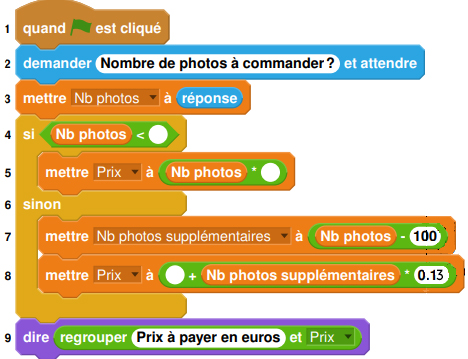
\includegraphics[scale=1]{FIG/scratch_fonction_cours.jpg} 

Par quelles valeurs peut-on compléter les instructions des lignes 4, 5 et 8 pour que
le programme permette de calculer le prix à payer en fonction du nombre de photos
commandées ?

\end{enumerate}


\end{ExoAuto}

  


%%%%%%%%%%%%%%%%%%%%%%%%%%%%%%%%%%%%%%%%%%%%%%%%%%%%%%%%%%%%%%%%%%%

 \begin{ExoAuto}{Chercher.}{1234}{2}{0}{0}{0}{0}
 
  
Pour ses 32 ans, Denis a acheté un vélo d'appartement afin de pouvoir s'entraîner pendant l'hiver.

La fréquence cardiaque (FC) est le nombre de pulsations (ou battements) du cœur par minute.

\medskip

\begin{enumerate}
\item Denis souhaite connaître sa fréquence cardiaque maximale conseillée (FCMC) afin de ne pas la dépasser et ainsi de ménager son cœur. La FCMC d'un individu dépend de son âge $a$, exprimé en années, elle peut s'obtenir grâce à la formule suivante établie par Astrand et Ryhming :
	
\begin{center}
\begin{tabularx}{0.8\linewidth}{|X|}\hline	
Fréquence cardiaque maximale conseillée = $220 - $âge.\\ \hline
\end{tabularx}
\end{center}

On note $f(a)$ la FCMC en fonction de l'âge $a$, on a donc $f(a) = 220 - a$.
	\begin{enumerate}
		\item Vérifier que la FCMC de Denis est égale à $188$ pulsations/minute. \point{2}
		\item Comparer la FCMC de Denis avec la FCMC d'une personne de $15$ ans. \point{4}
		\item La FCMC d'une personne est-elle proportionnelle à l'âge ?	Justifier.	 \point{4}
 	\end{enumerate}
\item  Après quelques recherches, Denis trouve une autre formule permettant d'obtenir sa FCMC de façon plus précise. Si $a$ désigne l'âge d'un individu, sa FCMC peut être calculée à l'aide de la formule de Gellish :
	
\begin{center}
\begin{tabularx}{0.9\linewidth}{|X|}\hline	
Fréquence cardiaque maximale conseillée = $191,5 - 0,007 \times \text{âge}^2$\rule[-3mm]{0mm}{8mm}\\ \hline
\end{tabularx}
\end{center}

On note $g(a)$ la FCMC en fonction de l'âge $a$, on a donc 

$g(a) = 191,5 - 0,007 \times a^2$.

Denis utilise un tableur pour comparer les résultats obtenus à l'aide des deux formules :

\begin{center}
\begin{tabularx}{\linewidth}{|c|c|*{2}{>{\centering \arraybackslash}X|}}\hline
\multicolumn{1}{|l}{B2}&\multicolumn{1}{l|}{~}&\multicolumn{1}{l|}{=220-A2}&\multicolumn{1}{l|}{~}\\ \hline
	&A 			&B 									&C\\ \hline
1	&Âge $a$	&FCMC $f(a)$ (Astrand et Ryhming)	&FCMC $g(a)$ (Gellish)\\ \hline
2	&30 		&190 								&185,2\\ \hline
3	&31 		&189 								&184,773\\ \hline
4	&32 		&188 								&184,332\\ \hline
5	&33 		&187 								&183,877\\ \hline
\end{tabularx}
\end{center}

Quelle formule faut-il insérer dans la cellule C2 puis recopier vers le bas, pour pouvoir compléter la colonne \og FCMC $g(a)$ (Gellish) \fg ?  \point{1}

\item Déterminer l'image de 31 par la fonction $g$. Justifier.\point{1}
\item Déterminer un antécédent de 188 par la fonction $f$. Justifier.\point{1}
\item Compléter la phrase :  187 est ............................................... de 33 par la fonction $f$. 
\end{enumerate}
 
 \end{ExoAuto}
 
 
\end{pageAuto}
%%%%%%%%%%%%%%%%%%%%%%%%%%%%%%%%%%%%%%%%%%%%%%%%%%%%%%%%%%%%%%%%%%%
%%%%  Brouillon
%%%%%%%%%%%%%%%%%%%%%%%%%%%%%%%%%%%%%%%%%%%%%%%%%%%%%%%%%%%%%%%%%%%


\begin{pageBrouillon} 
 
\ligne{32}



\end{pageBrouillon} %---------------> FAIT
%%%-----------
%%
%\chapter{Arithmétique}
{https://sacado.xyz/qcm/parcours_show_course/0/117129}
{
 \begin{CpsCol}
\textbf{Les savoir-faire du parcours}
 \begin{itemize}
 \item Calculer une longueur dans un triangle
 \end{itemize}
 
 \end{CpsCol}
 
 \begin{His}
 
\begin{wrapfigure}[15]{r}{3.6cm}
\vspace{-7mm}
\includegraphics[scale=0.5]{FIG/liebniz.jpg}

\begin{center}
  \textsc{Thalès} de Milet \\
  né à Milet vers 625-620 av. J.-C. et mort vers 548-545 av. J.-C
 \end{center} 
\end{wrapfigure}

\textbf{\textsc{Thalès}} est d'abord commerçant et ingénieur mais aussi homme politique.

Grâce à son séjour en Égypte, Thalès put mettre en œuvre ses connaissances en mathématiques, particulièrement en géométrie, domaines dans lesquels il fit quelques découvertes fondamentales, comme déterminer qu'un cercle est partagé en deux parties égales par tout diamètre ou que les angles à la base d'un triangle isocèle sont égaux. 

Ses découvertes astronomiques permirent d'aider à la navigation en haute mer en repérant certaines étoiles ou en déterminant les éphémérides. Il est probable que Thalès ait consigné ses découvertes par écrit afin d'en diffuser l'utilité, même s'il ne demeure à ce jour aucun texte de sa main.

En Europe, le théorème de Thalès ne désigne pas la même chose. En Allemagne,le « théorème de Thalès » porte sur l'angle inscrit dans un demi-cercle : si un triangle est inscrit dans un cercle avec un côté du triangle pour diamètre du cercle, alors ce triangle est rectangle d'hypoténuse ce diamètre.

 \end{His}

}




\begin{pageCours}




\section{Le théorème de Thalès}


\begin{ThT}{Le théorème de Thalès}\index{Théorème de Thalès}

Soit $(AB)$ et $(CD)$ deux droites sécantes en $O$.
 
Si les droites $\left(AC\right)$ et $\left(BD\right)$ sont parallèles alors on a :$\dfrac{OA}{OB}=\dfrac{OC}{OD}=\dfrac{AC}{BD}$.

\vspace{0.4cm}

\begin{minipage}{0.48\linewidth}
\begin{center}
Configuration en voile

\begin{tikzpicture}[line cap=round,line join=round,>=triangle 45,x=1.0cm,y=1.0cm]
\clip(2.32,1.02) rectangle (7.04,4.22);
\draw [line width=1.pt,color=xdxdff] (3.3,2.36)-- (6.36,1.84);
\draw [line width=1.pt,color=xdxdff] (6.36,1.84)-- (5.,3.32);
\draw [line width=1.pt,color=xdxdff] (5.,3.32)-- (3.3,2.36);
\draw [line width=1.pt,color=xdxdff,domain=2.32:7.04] plot(\x,{(--0.844--0.96*\x)/1.7});
\draw [line width=1.pt,color=xdxdff,domain=2.32:7.04] plot(\x,{(--8.9376-0.52*\x)/3.06});
\draw [line width=1.pt,color=xdxdff] (5.09733655157939,2.0545702592087305)-- (4.298520306432994,2.923870290691573);
\begin{scriptsize}
\draw [color=ududff] (3.3,2.36)-- ++(-2.5pt,0 pt) -- ++(5.0pt,0 pt) ++(-2.5pt,-2.5pt) -- ++(0 pt,5.0pt);
\draw[color=ududff] (3.1,2.69) node {$O$};
\draw [color=ududff] (6.36,1.84)-- ++(-2.5pt,0 pt) -- ++(5.0pt,0 pt) ++(-2.5pt,-2.5pt) -- ++(0 pt,5.0pt);
\draw[color=ududff] (6.42,1.61) node {$D$};
\draw [color=ududff] (5.,3.32)-- ++(-2.5pt,0 pt) -- ++(5.0pt,0 pt) ++(-2.5pt,-2.5pt) -- ++(0 pt,5.0pt);
\draw[color=ududff] (5.14,3.69) node {$B$};
\draw [color=xdxdff] (4.298520306432994,2.923870290691573)-- ++(-2.5pt,0 pt) -- ++(5.0pt,0 pt) ++(-2.5pt,-2.5pt) -- ++(0 pt,5.0pt);
\draw[color=xdxdff] (4.2,3.37) node {$A$};
\draw [color=xdxdff] (5.09733655157939,2.0545702592087305)-- ++(-2.5pt,0 pt) -- ++(5.0pt,0 pt) ++(-2.5pt,-2.5pt) -- ++(0 pt,5.0pt);
\draw[color=xdxdff] (5.02,1.81) node {$C$};
\end{scriptsize}
\end{tikzpicture}
\end{center}
\end{minipage}
\hfill
\begin{minipage}{0.48\linewidth}
\begin{center}
Configuration en papillon

\begin{tikzpicture}[line cap=round,line join=round,>=triangle 45,x=1.0cm,y=1.0cm]
\clip(-0.38,-0.5) rectangle (4.56,2.48);
\draw [line width=1.pt,color=xdxdff] (1.48,0.92)-- (3.02,0.46);
\draw [line width=1.pt,color=xdxdff] (3.02,0.46)-- (3.98,1.98);
\draw [line width=1.pt,color=xdxdff] (3.98,1.98)-- (1.48,0.92);
\draw [line width=1.pt,color=xdxdff,domain=-0.38:4.56] plot(\x,{(--0.7312--1.06*\x)/2.5});
\draw [line width=1.pt,color=xdxdff,domain=-0.38:4.56] plot(\x,{(--2.0976-0.46*\x)/1.54});
\draw [line width=1.pt,color=xdxdff] (0.5133438211999565,1.2087414560052079)-- (-0.08924704350656398,0.2546392535532169);
\begin{scriptsize}
\draw [color=ududff] (1.48,0.92)-- ++(-2.5pt,0 pt) -- ++(5.0pt,0 pt) ++(-2.5pt,-2.5pt) -- ++(0 pt,5.0pt);
\draw[color=ududff] (1.28,1.25) node {$O$};
\draw [color=ududff] (3.02,0.46)-- ++(-2.5pt,0 pt) -- ++(5.0pt,0 pt) ++(-2.5pt,-2.5pt) -- ++(0 pt,5.0pt);
\draw[color=ududff] (2.98,0.03) node {$D$};
\draw [color=ududff] (3.98,1.98)-- ++(-2.5pt,0 pt) -- ++(5.0pt,0 pt) ++(-2.5pt,-2.5pt) -- ++(0 pt,5.0pt);
\draw[color=ududff] (4.12,2.35) node {$A$};
\draw [color=xdxdff] (-0.08924704350656398,0.2546392535532169)-- ++(-2.5pt,0 pt) -- ++(5.0pt,0 pt) ++(-2.5pt,-2.5pt) -- ++(0 pt,5.0pt);
\draw[color=xdxdff] (0.18,0.07) node {$B$};
\draw [color=xdxdff] (0.5133438211999565,1.2087414560052079)-- ++(-2.5pt,0 pt) -- ++(5.0pt,0 pt) ++(-2.5pt,-2.5pt) -- ++(0 pt,5.0pt);
\draw[color=xdxdff] (0.66,1.57) node {$C$};
\end{scriptsize}
\end{tikzpicture}
\end{center}
\end{minipage}
\end{ThT}




\begin{ExCor}

\begin{minipage}{8.cm}

Sur la figure ci-contre, $\left(AC \right)$ est parallèle à $\left(BD \right)$.

\begin{itemize}
\item  $OA = 6$ cm ;
\item  $OB = 10$ cm ;
\item  $OC = 8$ cm.
\end{itemize}

Calculer $OD$.

\vspace{0.2cm}
 
\end{minipage}
\begin{minipage}{8.cm}

\begin{tikzpicture}[line cap=round,line join=round,>=triangle 45,x=1.0cm,y=1.0cm]
\clip(1.36,1.22) rectangle (6.96,4.34);
\draw [line width=1.pt,color=xdxdff] (1.72,2.2)-- (6.36,1.84);
\draw [line width=1.pt,color=xdxdff] (6.36,1.84)-- (5.,3.32);
\draw [line width=1.pt,color=xdxdff] (5.,3.32)-- (1.72,2.2);
\draw [line width=1.pt,color=xdxdff,domain=1.36:6.96] plot(\x,{(--5.2896--1.12*\x)/3.28});
\draw [line width=1.pt,color=xdxdff,domain=1.36:6.96] plot(\x,{(--10.8272-0.36*\x)/4.64});
\draw [line width=1.pt,color=xdxdff] (4.445373071675939,1.9885486409906603)-- (3.6465568265295425,2.8578486724735024);
\begin{scriptsize}
\draw [color=ududff] (1.72,2.2)-- ++(-2.5pt,0 pt) -- ++(5.0pt,0 pt) ++(-2.5pt,-2.5pt) -- ++(0 pt,5.0pt);
\draw[color=ududff] (1.52,2.53) node {$O$};
\draw [color=ududff] (6.36,1.84)-- ++(-2.5pt,0 pt) -- ++(5.0pt,0 pt) ++(-2.5pt,-2.5pt) -- ++(0 pt,5.0pt);
\draw[color=ududff] (6.42,1.61) node {$D$};
\draw [color=ududff] (5.,3.32)-- ++(-2.5pt,0 pt) -- ++(5.0pt,0 pt) ++(-2.5pt,-2.5pt) -- ++(0 pt,5.0pt);
\draw[color=ududff] (5.14,3.69) node {$B$};
\draw[color=xdxdff] (-4.08,0.55) node {$f$};
\draw[color=xdxdff] (-4.08,2.51) node {$g$};
\draw [color=xdxdff] (3.6465568265295425,2.8578486724735024)-- ++(-2.5pt,0 pt) -- ++(5.0pt,0 pt) ++(-2.5pt,-2.5pt) -- ++(0 pt,5.0pt);
\draw[color=xdxdff] (3.54,3.31) node {$A$};
\draw [color=xdxdff] (4.445373071675939,1.9885486409906603)-- ++(-2.5pt,0 pt) -- ++(5.0pt,0 pt) ++(-2.5pt,-2.5pt) -- ++(0 pt,5.0pt);
\draw[color=xdxdff] (4.36,1.73) node {$C$};
\end{scriptsize}
\end{tikzpicture}

\end{minipage}
\begin{minipage}{1.5cm}
\colorbox{sacado_blue}{\miniqr{1234}}
\end{minipage}
 
\begin{minipage}{10cm}
\begin{itemize}[leftmargin=*]
\item Les droites $(AB)$ et $(CD)$ sont sécantes en $O$. 
\item La droite $\left(AC \right)$ est parallèle à $\left( BD \right)$
\end{itemize}
\end{minipage}
\begin{minipage}{8cm}
 {\color{sacado_blue}\textbf{[1. Contexte de la situation]}}
\end{minipage}

\vspace{0.1cm}

Donc, d'après le théorème de Thalès, $\frac{OA}{OB}=\frac{OC}{OD}=\frac{AC}{BD}$ {\color{sacado_blue}\textbf{[2. Écrire les égalités des trois quotients]}}

Donc $\dfrac{6}{10}=\dfrac{8}{OD}=\dfrac{AC}{BD}$ {\color{sacado_blue}\textbf{[3. Remplacer les valeurs connues]}}

Comme $\dfrac{6}{10}=\dfrac{8}{OD}$ {\color{sacado_blue}\textbf{[4. Conserver généralement une seule égalité]}}

On déduit que $6\times OD=8 \times 10$ {\color{sacado_blue}\textbf{[5. Écrire de l'égalité à partir du produit en croix]}}

$OD= \dfrac{8 \times 10}{6}= \dfrac{8 \times 5}{3}= \dfrac{40}{3}$  (on \og isole \fg{} la longueur cherchée) et donc $OD=\dfrac{40}{3}$ cm {\color{sacado_blue}\textbf{[6. Conclure]}}.
\end{ExCor}











\begin{ExCor}

\begin{minipage}{8.cm}

Sur la figure ci-contre, $\left(YT\right)$ est parallèle à $\left(OJ\right)$.

\begin{itemize}
\item  $RT = 3$ cm ;
\item  $RO = 5$ cm ;
\item  $RY = 4,5$ cm.
\end{itemize}

Calculer $RJ$.

\vspace{0.2cm}
 
\end{minipage}
\begin{minipage}{8.cm}

\begin{tikzpicture}[line cap=round,line join=round,>=triangle 45,x=1.0cm,y=1.0cm]
\clip(0.1,0.74) rectangle (6.58,4.04);
\draw [line width=1.pt,color=xdxdff] (3.3,2.36)-- (5.66,1.74);
\draw [line width=1.pt,color=xdxdff] (5.66,1.74)-- (5.,3.32);
\draw [line width=1.pt,color=xdxdff] (5.,3.32)-- (3.3,2.36);
\draw [line width=1.pt,color=xdxdff,domain=0.1:6.58] plot(\x,{(--0.844--0.96*\x)/1.7});
\draw [line width=1.pt,color=xdxdff,domain=0.1:6.58] plot(\x,{(--7.6156-0.62*\x)/2.36});
\draw [line width=1.pt,color=xdxdff] (0.8507670608657913,3.003442551806444)-- (1.5357220353694259,1.3637018552674407);
\begin{scriptsize}
\draw [color=xdxdff] (3.3,2.36)-- ++(-2.5pt,0 pt) -- ++(5.0pt,0 pt) ++(-2.5pt,-2.5pt) -- ++(0 pt,5.0pt);
\draw[color=xdxdff] (3.1,2.69) node {$R$};
\draw [color=xdxdff] (5.66,1.74)-- ++(-2.5pt,0 pt) -- ++(5.0pt,0 pt) ++(-2.5pt,-2.5pt) -- ++(0 pt,5.0pt);
\draw[color=xdxdff] (5.62,1.31) node {$Y$};
\draw [color=xdxdff] (5.,3.32)-- ++(-2.5pt,0 pt) -- ++(5.0pt,0 pt) ++(-2.5pt,-2.5pt) -- ++(0 pt,5.0pt);
\draw[color=xdxdff] (5.14,3.69) node {$T$};
\draw [color=xdxdff] (1.5357220353694259,1.3637018552674407)-- ++(-2.5pt,0 pt) -- ++(5.0pt,0 pt) ++(-2.5pt,-2.5pt) -- ++(0 pt,5.0pt);
\draw[color=xdxdff] (1.8,1.17) node {$O$};
\draw [color=xdxdff] (0.8507670608657913,3.003442551806444)-- ++(-2.5pt,0 pt) -- ++(5.0pt,0 pt) ++(-2.5pt,-2.5pt) -- ++(0 pt,5.0pt);
\draw[color=xdxdff] (0.76,3.39) node {$J$};
\end{scriptsize}
\end{tikzpicture}

\end{minipage}
\begin{minipage}{1.5cm}
\colorbox{sacado_blue}{\miniqr{1234}}
\end{minipage}
 
\begin{minipage}{10cm}
\begin{itemize}[leftmargin=*]
\item Les droites $(JY)$ et $(OT)$ sont sécantes en $R$. 
\item La droite $\left(YT\right)$ est parallèle à $\left(OJ\right)$
\end{itemize}
\end{minipage}
\begin{minipage}{8cm}
 {\color{sacado_blue}\textbf{[1. Contexte de la situation]}}
\end{minipage}

\vspace{0.1cm}

Donc, d'après le théorème de Thalès, $\dfrac{RY}{RJ}=\dfrac{RT}{RO}=\dfrac{YT}{JO}$ {\color{sacado_blue}\textbf{[2. Écrire les égalités des trois quotients]}}

Donc $\dfrac{4,5}{RJ}=\dfrac{3}{5}=\dfrac{YT}{JO}$ {\color{sacado_blue}\textbf{[3. Remplacer les valeurs connues]}}

Donc $\dfrac{4,5}{RJ}=\dfrac{3}{5}$ {\color{sacado_blue}\textbf{[4. Conserver généralement une seule égalité]}}

On déduit que $4,5 \times 5=3\times RJ$ {\color{sacado_blue}\textbf{[5. Écrire de l'égalité à partir du produit en croix]}}

$RJ= \dfrac{4,5 \times 5}{3}$  (on \og isole \fg{} la longueur cherchée) et donc $RJ=7,5$ cm {\color{sacado_blue}\textbf{[6. Conclure]}}.
\end{ExCor}


\end{pageCours} 
\begin{pageAD} 
 

\Sf{Reconnaitre une situation de Thalès.}
 
\begin{ExoCad}{Modéliser. Calculer.}{1234}{0}{0}{0}{0}{0}

Écrire le théorème de Thalès associé à chaque configuration.

\begin{minipage}{0.48\linewidth}

\definecolor{xdxdff}{rgb}{0.49019607843137253,0.49019607843137253,1.}
\definecolor{qqqqff}{rgb}{0.,0.,1.}
\definecolor{ududff}{rgb}{0.30196078431372547,0.30196078431372547,1.}
\begin{tikzpicture}[line cap=round,line join=round,>=triangle 45,x=1.0cm,y=1.0cm]
\clip(0.14,0.5) rectangle (6.04,4.5);
\draw [line width=1.pt,color=xdxdff] (1.,1.)-- (5.4,1.18);
\draw [line width=1.pt,color=xdxdff] (5.4,1.18)-- (3.98,3.78);
\draw [line width=1.pt,color=xdxdff] (3.98,3.78)-- (1.,1.);
\draw [line width=1.pt,color=xdxdff] (2.8840981002867094,2.7576485633547154)-- (3.7818898125038674,1.1138045832387946);
\begin{scriptsize}
\draw [color=xdxdff] (1.,1.)-- ++(-2.5pt,0 pt) -- ++(5.0pt,0 pt) ++(-2.5pt,-2.5pt) -- ++(0 pt,5.0pt);
\draw[color=xdxdff] (0.8,1.33) node {$A$};
\draw [color=xdxdff] (5.4,1.18)-- ++(-2.5pt,0 pt) -- ++(5.0pt,0 pt) ++(-2.5pt,-2.5pt) -- ++(0 pt,5.0pt);
\draw[color=xdxdff] (5.64,1.21) node {$B$};
\draw [color=xdxdff] (3.98,3.78)-- ++(-2.5pt,0 pt) -- ++(5.0pt,0 pt) ++(-2.5pt,-2.5pt) -- ++(0 pt,5.0pt);
\draw[color=xdxdff] (4.12,4.15) node {$C$};
\draw [color=xdxdff] (3.7818898125038674,1.1138045832387946)-- ++(-2.5pt,0 pt) -- ++(5.0pt,0 pt) ++(-2.5pt,-2.5pt) -- ++(0 pt,5.0pt);
\draw[color=xdxdff] (4.08,0.91) node {$D$};
\draw [color=qqqqff] (2.8840981002867094,2.7576485633547154)-- ++(-2.0pt,0 pt) -- ++(4.0pt,0 pt) ++(-2.0pt,-2.0pt) -- ++(0 pt,4.0pt);
\draw[color=qqqqff] (3.,3.23) node {$E$};
\end{scriptsize}
\end{tikzpicture}

\point{6}
\end{minipage}
\hfill
\begin{minipage}{0.48\linewidth}

\definecolor{xdxdff}{rgb}{0.49019607843137253,0.49019607843137253,1.}
\definecolor{qqqqff}{rgb}{0.,0.,1.}
\definecolor{ududff}{rgb}{0.30196078431372547,0.30196078431372547,1.}
\begin{tikzpicture}[line cap=round,line join=round,>=triangle 45,x=1.0cm,y=1.0cm]
\clip(-1.08,-0.56) rectangle (5.42,2.52);
\draw [line width=1.pt,color=xdxdff] (1.48,0.92)-- (4.76,0.3);
\draw [line width=1.pt,color=xdxdff] (4.76,0.3)-- (3.98,1.98);
\draw [line width=1.pt,color=xdxdff] (3.98,1.98)-- (1.48,0.92);
\draw [line width=1.pt,color=xdxdff,domain=-1.08:5.42] plot(\x,{(--0.7312--1.06*\x)/2.5});
\draw [line width=1.pt,color=xdxdff,domain=-1.08:5.42] plot(\x,{(--3.9352-0.62*\x)/3.28});
\draw [line width=1.pt,color=xdxdff] (-0.5788521210806118,1.3091732667896279)-- (-0.08924704350656393,0.2546392535532168);
\begin{scriptsize}
\draw [color=xdxdff] (1.48,0.92)-- ++(-2.5pt,0 pt) -- ++(5.0pt,0 pt) ++(-2.5pt,-2.5pt) -- ++(0 pt,5.0pt);
\draw[color=xdxdff] (1.28,1.25) node {$A$};
\draw [color=xdxdff] (4.76,0.3)-- ++(-2.5pt,0 pt) -- ++(5.0pt,0 pt) ++(-2.5pt,-2.5pt) -- ++(0 pt,5.0pt);
\draw[color=xdxdff] (4.72,-0.13) node {$B$};
\draw [color=xdxdff] (3.98,1.98)-- ++(-2.5pt,0 pt) -- ++(5.0pt,0 pt) ++(-2.5pt,-2.5pt) -- ++(0 pt,5.0pt);
\draw[color=xdxdff] (4.12,2.35) node {$C$};
\draw [color=xdxdff] (-0.08924704350656393,0.2546392535532168)-- ++(-2.5pt,0 pt) -- ++(5.0pt,0 pt) ++(-2.5pt,-2.5pt) -- ++(0 pt,5.0pt);
\draw[color=xdxdff] (0.18,0.07) node {$D$};
\draw [color=xdxdff] (-0.5788521210806118,1.3091732667896279)-- ++(-2.5pt,0 pt) -- ++(5.0pt,0 pt) ++(-2.5pt,-2.5pt) -- ++(0 pt,5.0pt);
\draw[color=xdxdff] (-0.44,1.67) node {$E$};
\end{scriptsize}
\end{tikzpicture}


\point{6}
\end{minipage}


\end{ExoCad}

 
\Sf{Calculer une longueur avec le théorème de Thalès.}

\begin{ExoCad}{Calculer.}{1234}{0}{0}{0}{0}{0}


\begin{minipage}{0.48\linewidth}

\definecolor{xdxdff}{rgb}{0.49019607843137253,0.49019607843137253,1.}
\definecolor{qqqqff}{rgb}{0.,0.,1.}
\definecolor{ududff}{rgb}{0.30196078431372547,0.30196078431372547,1.}
\begin{tikzpicture}[line cap=round,line join=round,>=triangle 45,x=1.0cm,y=1.0cm]
\clip(0.14,0.5) rectangle (6.04,4.5);
\draw [line width=1.pt,color=xdxdff] (1.,1.)-- (5.4,1.18);
\draw [line width=1.pt,color=xdxdff] (5.4,1.18)-- (3.98,3.78);
\draw [line width=1.pt,color=xdxdff] (3.98,3.78)-- (1.,1.);
\draw [line width=1.pt,color=xdxdff] (2.8840981002867094,2.7576485633547154)-- (3.7818898125038674,1.1138045832387946);
\begin{scriptsize}
\draw [color=xdxdff] (1.,1.)-- ++(-2.5pt,0 pt) -- ++(5.0pt,0 pt) ++(-2.5pt,-2.5pt) -- ++(0 pt,5.0pt);
\draw[color=xdxdff] (0.8,1.33) node {$R$};
\draw [color=xdxdff] (5.4,1.18)-- ++(-2.5pt,0 pt) -- ++(5.0pt,0 pt) ++(-2.5pt,-2.5pt) -- ++(0 pt,5.0pt);
\draw[color=xdxdff] (5.64,1.21) node {$A$};
\draw [color=xdxdff] (3.98,3.78)-- ++(-2.5pt,0 pt) -- ++(5.0pt,0 pt) ++(-2.5pt,-2.5pt) -- ++(0 pt,5.0pt);
\draw[color=xdxdff] (4.12,4.15) node {$T$};
\draw [color=xdxdff] (3.7818898125038674,1.1138045832387946)-- ++(-2.5pt,0 pt) -- ++(5.0pt,0 pt) ++(-2.5pt,-2.5pt) -- ++(0 pt,5.0pt);
\draw[color=xdxdff] (4.08,0.91) node {$I$};
\draw [color=qqqqff] (2.8840981002867094,2.7576485633547154)-- ++(-2.0pt,0 pt) -- ++(4.0pt,0 pt) ++(-2.0pt,-2.0pt) -- ++(0 pt,4.0pt);
\draw[color=qqqqff] (3.,3.23) node {$Z$};
\end{scriptsize}
\end{tikzpicture}

Les droites $(AT)$ et $(IZ)$ sont parallèles. $RA=8$, 

$RI=5$, $AT=7$. 

Calculer $IZ$.
\end{minipage}
\begin{minipage}{0.48\linewidth}
\point{10}
\end{minipage}
\end{ExoCad}



\begin{ExoCad}{Calculer.}{1234}{0}{0}{0}{0}{0}
 
\begin{minipage}{0.48\linewidth}
\begin{tikzpicture}[line cap=round,line join=round,>=triangle 45,x=1.0cm,y=1.0cm]
\clip(0.06,1.26) rectangle (6.92,4.88);
\draw [line width=1.pt,color=xdxdff] (3.12,3.02)-- (5.28,2.14);
\draw [line width=1.pt,color=xdxdff] (5.28,2.14)-- (6.4,4.14);
\draw [line width=1.pt,color=xdxdff] (6.4,4.14)-- (3.12,3.02);
\draw [line width=1.pt,color=xdxdff,domain=0.06:6.92] plot(\x,{(--6.4112--1.12*\x)/3.28});
\draw [line width=1.pt,color=xdxdff,domain=0.06:6.92] plot(\x,{(--9.2688-0.88*\x)/2.16});
\draw [line width=1.pt,color=xdxdff] (1.508630793819925,3.676483750665956)-- (0.6731060202450717,2.184475226425147);
\begin{scriptsize}
\draw [color=ududff] (3.12,3.02)-- ++(-2.5pt,0 pt) -- ++(5.0pt,0 pt) ++(-2.5pt,-2.5pt) -- ++(0 pt,5.0pt);
\draw[color=ududff] (2.92,3.35) node {$A$};
\draw [color=ududff] (5.28,2.14)-- ++(-2.5pt,0 pt) -- ++(5.0pt,0 pt) ++(-2.5pt,-2.5pt) -- ++(0 pt,5.0pt);
\draw[color=ududff] (5.34,1.91) node {$V$};
\draw [color=ududff] (6.4,4.14)-- ++(-2.5pt,0 pt) -- ++(5.0pt,0 pt) ++(-2.5pt,-2.5pt) -- ++(0 pt,5.0pt);
\draw[color=ududff] (6.54,4.51) node {$E$};
\draw [color=xdxdff] (0.6731060202450717,2.184475226425147)-- ++(-2.5pt,0 pt) -- ++(5.0pt,0 pt) ++(-2.5pt,-2.5pt) -- ++(0 pt,5.0pt);
\draw[color=xdxdff] (0.58,2.63) node {$U$};
\draw [color=xdxdff] (1.508630793819925,3.676483750665956)-- ++(-2.5pt,0 pt) -- ++(5.0pt,0 pt) ++(-2.5pt,-2.5pt) -- ++(0 pt,5.0pt);
\draw[color=xdxdff] (1.52,4.13) node {$C$};
\end{scriptsize}
\end{tikzpicture}
 
 
 Les droites $(UC)$ et $(EV)$ sont parallèles. 
 
 $CA=5$cm, $CU=6$cm, $AV=7$cm. 

Calculer $EV$.
\end{minipage}
\begin{minipage}{0.48\linewidth}
\point{10}
\end{minipage}
\end{ExoCad}

 




\end{pageAD}

\begin{pageCours}

\section{Agrandissement et Réduction}

\begin{DefT}{Agrandissement et Réduction}\index{Agrandissement}\index{Réduction}
Si	deux figures ont la même forme et des longueurs proportionnelles, 
alors on dit que l'une est un \textbf{agrandissement ou une réduction} de l'autre.
\end{DefT}

\begin{Rq}
Le coefficient de proportionnalité $k$ est le rapport d'agrandissement ou de réduction.
\end{Rq}

\begin{Rq} 
\begin{itemize}[leftmargin=*]
\item  Les dimensions du triangle $OAC$ sont proportionnelles aux dimensions du triangle $OBD$.
\item  Le coefficient de proportionnalité est $\dfrac{OA}{OB}$ ou $\dfrac{OC}{OD}$ ou encore $\dfrac{AC}{BD}$. Lorsque ce rapport est supérieur à 1, on parle d'\textbf{agrandissement} sinon on parle de \textbf{réduction}.
\item  Dans ces configurations, on dit que les triangles sont \textbf{semblables}.\index{Triangles semblables}
\end{itemize}
\end{Rq}


\begin{ExCor}

\begin{minipage}{0.48\linewidth}
Le triangle $ABC$ a les dimensions suivantes.
\\$AB = 1,5$ cm
\\$BC = 2,5$ cm
\\$AC = 3,2$ cm

$DEF$ est un agrandissement de $ABC$ de rapport $1,6$. 

Calculer le périmètre $\mathcal{P}$ du triangle $DEF$.
\end{minipage}
\begin{minipage}{0.48\linewidth}
$DE = 1,6 \times AB = 1,6 \times 1,5 = 2,4$ cm

$DF = 1,6 \times AC = 1,6 \times 2,5 = 4$ cm

$EF = 1,6 \times BC = 1,6 \times 3,2 = 5,12$ cm

$\mathcal{P} = 2,4 + 4 + 5,12 = 11,52 (= 1,6 \times 7,2) $cm
\end{minipage}

\end{ExCor}

\begin{Rq} 
\begin{itemize}
\item $ABC$ est une réduction de $DEF$ de rapport $\dfrac{1,5}{2,4}  = \dfrac{2,5}{4} =\dfrac{3,2}{5,12}  = 0,625$.
\item Dans un agrandissement ou une réduction, les mesures des angles, la perpendicularité 
et le parallélisme sont conservés.
\end{itemize}
\end{Rq}



\begin{ThT}{Rapport d'agrandissement et/ou de réduction}\index{Rapport d'aires}\index{Rapport de volumes}
Si $k$ est le rapport de proportion de longueur alors :
\begin{itemize}[leftmargin=*]
\item  les aires sont multipliées par $k^2$.
\item  les volumes sont multipliés par $k^3$.
\end{itemize}
\end{ThT}




\end{pageCours} 
\begin{pageAD} 
 
\Sf{Calculer un coefficient d'agrandissement ou de réduction.}


\begin{ExoCad}{Calculer.}{1234}{0}{0}{0}{0}{0}

 

\end{ExoCad}



\end{pageAD}
%%%%%%%%%%%%%%%%%%%%%%%%%%%%%%%%%%%%%%%%%%%%%%%%%%%%%%%%%%%%%%%%%%%
%%%%  Niveau 1
%%%%%%%%%%%%%%%%%%%%%%%%%%%%%%%%%%%%%%%%%%%%%%%%%%%%%%%%%%%%%%%%%%%
\begin{pageParcoursu} 

 %%%%%%%%%%%%%%%%%%%%%%%%%%%
 

\begin{ExoCu}{Communiquer.}{1234}{0}{0}{0}{0}{0}

Soit $EFGH$ un parallélogramme tel que $EF=4$~cm; $FH=5$~cm et
$EH=6$~cm. \\Soit $K$ le point du segment $[EH]$ tel que
$HK=1,2$~cm.\\La parallèle à la droite $(EF)$ passant par $K$ coupe le
segment $[FH]$ en $J$.\par Calculer les longueurs $HJ$ et $JK$.

\end{ExoCu}


\begin{ExoCu}{Communiquer.}{1234}{0}{0}{0}{0}{0}


\end{ExoCu}

 

\begin{ExoCu}{DNB 2023 - Modéliser. Calculer.}{1234}{0}{0}{0}{0}{0}

Marie se place comme indiquée sur la figure ci-dessous, de telle sorte que son ombre coïncide avec celle de la tour. Après avoir effectué plusieurs mesures, Adrien effectue le schéma ci- dessous (le schéma n'est pas à l'échelle), sur lequel les points A, E et B ainsi que les points A, D et C sont alignés.

Calculer la hauteur BC de la Gyrotour.


\begin{center}
\definecolor{qqqqff}{rgb}{0.,0.,1.}
\definecolor{qqqqcc}{rgb}{0.,0.,0.8}
\begin{tikzpicture}[line cap=round,line join=round,>=triangle 45,x=1.0cm,y=1.0cm]
\clip(-4.2,-3.7) rectangle (7.56,2.56);
\draw[line width=2.pt,color=qqqqcc] (-0.5757359312880717,-3.) -- (-0.5757359312880715,-2.5757359312880714) -- (-1.,-2.5757359312880714) -- (-1.,-3.) -- cycle; 
\draw[line width=2.pt,color=qqqqcc] (7.,-2.5757359312880714) -- (6.575735931288071,-2.5757359312880714) -- (6.575735931288071,-3.) -- (7.,-3.) -- cycle; 
\draw [line width=2.pt,color=qqqqcc] (-4.,-3.)-- (7.,2.);
\draw [line width=2.pt,color=qqqqcc] (7.,2.)-- (7.,-3.);
\draw [line width=2.pt,color=qqqqcc] (7.,-3.)-- (-1.,-3.);
\draw [line width=2.pt,color=qqqqcc] (-4.,-3.)-- (-1.,-3.);
\draw [line width=2.pt,color=qqqqff] (-1.,-1.6363636363636365)-- (-1.,-3.);
\draw (-0.84,-1.66) node[anchor=north west] {$160 \;cm$};
\draw (2.06,-2.82) node[anchor=north west] {$54,25\;m$};
\draw (-2.94,-2.82) node[anchor=north west] {$2\;m$};
\begin{scriptsize}
\draw [color=qqqqcc] (-4.,-3.)-- ++(-2.5pt,0 pt) -- ++(5.0pt,0 pt) ++(-2.5pt,-2.5pt) -- ++(0 pt,5.0pt);
\draw[color=qqqqcc] (-4.04,-3.33) node {$A$};
\draw [color=qqqqcc] (7.,2.)-- ++(-2.5pt,0 pt) -- ++(5.0pt,0 pt) ++(-2.5pt,-2.5pt) -- ++(0 pt,5.0pt);
\draw[color=qqqqcc] (7.14,2.37) node {$B$};
\draw [color=qqqqcc] (7.,-3.)-- ++(-2.5pt,0 pt) -- ++(5.0pt,0 pt) ++(-2.5pt,-2.5pt) -- ++(0 pt,5.0pt);
\draw[color=qqqqcc] (7.14,-2.63) node {$C$};
\draw [color=qqqqcc] (-1.,-3.)-- ++(-2.5pt,0 pt) -- ++(5.0pt,0 pt) ++(-2.5pt,-2.5pt) -- ++(0 pt,5.0pt);
\draw[color=qqqqcc] (-0.9,-3.17) node {$D$};
\draw [color=qqqqcc] (-1.,-1.6363636363636365)-- ++(-2.5pt,0 pt) -- ++(5.0pt,0 pt) ++(-2.5pt,-2.5pt) -- ++(0 pt,5.0pt);
\draw[color=qqqqcc] (-0.86,-1.27) node {$E$};
\end{scriptsize}
\end{tikzpicture}

\end{center}

\end{ExoCu}

 
\end{pageParcoursu}

  
%%%%%%%%%%%%%%%%%%%%%%%%%%%%%%%%%%%%%%%%%%%%%%%%%%%%%%%%%%%%%%%%%%%
%%%%  Niveau 2
%%%%%%%%%%%%%%%%%%%%%%%%%%%%%%%%%%%%%%%%%%%%%%%%%%%%%%%%%%%%%%%%%%%



\begin{pageParcoursd} 
 
%%%%%%%%%%%%%%%%%%%%%%%%%%%%%%%%%%%%%%%%%%%%%%%%%%%%%%%%%%%%%%%%%%%


 

 
 
\begin{ExoCd}{Calculer.}{1234}{0}{0}{0}{0}{0}

Construis un triangle $RST$ tel que $RS=8,8$~cm; $RT=5,6$~cm et
 $ST=4,8$~cm.  Soit $M$ le point du segment $[RS]$ tel que
 $RM=6,6$~cm.\\La parallèle à la droite $(ST)$ passant par $M$
 coupe le segment $[RT]$ en $N$.
\begin{enumerate}[leftmargin=*]
\item Calcule la longueur $MN$.
\item Calcule la longueur $RN$. Déduis-en la longueur $NT$.
\end{enumerate}

\end{ExoCd}
 

\begin{ExoCd}{Calculer.}{1234}{0}{0}{0}{0}{0}


La tour de la Vade est un monument de Carcassonne.


 Afin de déterminer la hauteur de cette tour, Romane et Maël se sont positionnés comme indiqué sur la figure ci-dessous, et ont effectué plusieurs mesures.

L'oeil de Maël est au point M ; le segment [FG] représente Romane.

La figure n'est pas à l'échelle.

\begin{center}

\definecolor{xdxdff}{rgb}{0.49019607843137253,0.49019607843137253,1.}
\definecolor{ttttff}{rgb}{0.2,0.2,1.}
\begin{tikzpicture}[line cap=round,line join=round,>=triangle 45,x=1.0cm,y=1.0cm]
\clip(-3.58,0.42) rectangle (7.92,4.66);
\draw (1.06,2.18) node[anchor=north west] {$Romane$};
\draw (-3.42,1.14) node[anchor=north west] {$Maël$};
\draw (6.32,2.98) node[anchor=north west] {$Tour$};
\draw [line width=2.pt] (-3.,1.)-- (6.,1.);
\draw [line width=2.pt] (-3.,1.)-- (6.,4.);
\draw [line width=2.pt] (6.,4.)-- (6.,1.);
\draw [line width=2.pt] (6.,1.)-- (7.48,1.);
\draw [line width=2.pt] (7.48,1.)-- (7.48,3.98);
\draw [line width=2.pt] (7.48,3.98)-- (6.,4.);
\draw [line width=2.pt] (1.,1.)-- (0.996,2.332);
\begin{scriptsize}
\draw [color=ttttff] (-3.,1.)-- ++(-2.0pt,0 pt) -- ++(4.0pt,0 pt) ++(-2.0pt,-2.0pt) -- ++(0 pt,4.0pt);
\draw[color=ttttff] (-3.38,1.17) node {$M$};
\draw [color=ttttff] (6.,1.)-- ++(-2.0pt,0 pt) -- ++(4.0pt,0 pt) ++(-2.0pt,-2.0pt) -- ++(0 pt,4.0pt);
\draw[color=ttttff] (6.14,1.33) node {$B$};
\draw [color=ttttff] (6.,4.)-- ++(-2.0pt,0 pt) -- ++(4.0pt,0 pt) ++(-2.0pt,-2.0pt) -- ++(0 pt,4.0pt);
\draw[color=ttttff] (6.14,4.33) node {$A$};
\draw [color=ttttff] (7.48,1.)-- ++(-2.0pt,0 pt) -- ++(4.0pt,0 pt) ++(-2.0pt,-2.0pt) -- ++(0 pt,4.0pt);
\draw[color=ttttff] (7.62,1.33) node {$C$};
\draw [color=ttttff] (7.48,3.98)-- ++(-2.0pt,0 pt) -- ++(4.0pt,0 pt) ++(-2.0pt,-2.0pt) -- ++(0 pt,4.0pt);
\draw[color=ttttff] (7.62,4.31) node {$D$};
\draw [color=xdxdff] (1.,1.)-- ++(-1.0pt,0 pt) -- ++(2.0pt,0 pt) ++(-1.0pt,-1.0pt) -- ++(0 pt,2.0pt);
\draw[color=xdxdff] (0.88,0.83) node {$G$};
\draw [color=xdxdff] (0.996,2.332)-- ++(-1.0pt,0 pt) -- ++(2.0pt,0 pt) ++(-1.0pt,-1.0pt) -- ++(0 pt,2.0pt);
\draw[color=xdxdff] (1.14,2.59) node {$F$};
\end{scriptsize}
\end{tikzpicture}



\end{center}

Les points M, F et A ainsi que les points M, G et B sont alignés.

Romane et Maël ont mesuré : MG $= 3$~m

\phantom{Romane et Maël ont mesuré : }FG $= 1,4$ m

\phantom{Romane et Maël ont mesuré : }GB $= 51$ m

	\begin{enumerate}
		\item Montrer que les droites (FG) et (AB) sont parallèles. 
		\item Vérifier que la hauteur AB de la tour est de $25,2$~m.
	\end{enumerate}	

\end{ExoCd}
 
 
 
\begin{ExoCd}{DNB 2022 - Représenter.}{1234}{0}{0}{0}{0}{0}

\begin{minipage}{0.6\linewidth}

Pour une épreuve d'orientation, Aurore reçoit
le plan ci-contre. Sachant que les droites $(EF)$ et $(IA)$ sont
parallèles ainsi que les droites $(GH)$ et $(DA)$, quelle est la
longueur du parcours $DEFGHA$ ?

\vspace{5mm}

$D$ : Départ\kern1cm $A$ : arrivée.\\
$DA=600$~m; $DE=200$~m; $IG=90$~m; $DI=315$~m; $IA=390$~m.
\end{minipage}
\begin{minipage}{0.4\linewidth}

 \definecolor{dcrutc}{rgb}{0.8627450980392157,0.0784313725490196,0.23529411764705882}
\definecolor{ududff}{rgb}{0.30196078431372547,0.30196078431372547,1.}
\definecolor{qqqqff}{rgb}{0.,0.,1.}
\definecolor{xdxdff}{rgb}{0.49019607843137253,0.49019607843137253,1.}
\begin{tikzpicture}[line cap=round,line join=round,>=triangle 45,x=1.0cm,y=1.0cm]
\clip(-2.66,-2.48) rectangle (5.48,4.76);
\draw [line width=2.pt,color=qqqqff] (-2.,4.)-- (5.,4.);
\draw [line width=2.pt,color=qqqqff] (5.,4.)-- (0.,-2.);
\draw [line width=2.pt,color=qqqqff] (0.,-2.)-- (-2.,4.);
\draw [line width=2.pt,color=dcrutc] (5.,4.)-- (1.31,-0.428);
\draw [line width=2.pt,color=dcrutc] (1.31,-0.428)-- (-0.524,-0.428);
\draw [line width=2.pt,color=dcrutc] (-0.524,-0.428)-- (-1.4285714285714286,2.2857142857142856);
\draw [line width=2.pt,color=dcrutc] (-1.4285714285714286,2.2857142857142856)-- (0.,4.);
\draw [line width=2.pt,color=dcrutc] (0.,4.)-- (-2.,4.);
\begin{scriptsize}
\draw [color=xdxdff] (-2.,4.)-- ++(-2.5pt,0 pt) -- ++(5.0pt,0 pt) ++(-2.5pt,-2.5pt) -- ++(0 pt,5.0pt);
\draw[color=xdxdff] (-1.86,4.37) node {$D$};
\draw [color=xdxdff] (5.,4.)-- ++(-2.5pt,0 pt) -- ++(5.0pt,0 pt) ++(-2.5pt,-2.5pt) -- ++(0 pt,5.0pt);
\draw[color=xdxdff] (5.14,4.37) node {$A$};
\draw[color=qqqqff] (1.56,3.85) node {$f$};
\draw [color=ududff] (0.,-2.)-- ++(-2.5pt,0 pt) -- ++(5.0pt,0 pt) ++(-2.5pt,-2.5pt) -- ++(0 pt,5.0pt);
\draw[color=ududff] (0.28,-2.09) node {$I$};
\draw[color=qqqqff] (2.3,1.39) node {$g$};
\draw[color=qqqqff] (-0.64,1.29) node {$h$};
\draw [color=xdxdff] (0.,4.)-- ++(-2.5pt,0 pt) -- ++(5.0pt,0 pt) ++(-2.5pt,-2.5pt) -- ++(0 pt,5.0pt);
\draw[color=xdxdff] (0.14,4.37) node {$E$};
\draw [color=xdxdff] (-1.4285714285714286,2.2857142857142856)-- ++(-2.0pt,0 pt) -- ++(4.0pt,0 pt) ++(-2.0pt,-2.0pt) -- ++(0 pt,4.0pt);
\draw[color=xdxdff] (-1.76,2.35) node {$F$};
\draw [color=xdxdff] (-0.524,-0.428)-- ++(-2.5pt,0 pt) -- ++(5.0pt,0 pt) ++(-2.5pt,-2.5pt) -- ++(0 pt,5.0pt);
\draw[color=xdxdff] (-0.96,-0.45) node {$C$};
\draw [color=xdxdff] (1.31,-0.428)-- ++(-2.5pt,0 pt) -- ++(5.0pt,0 pt) ++(-2.5pt,-2.5pt) -- ++(0 pt,5.0pt);
\draw[color=xdxdff] (1.62,-0.51) node {$H$};
\end{scriptsize}
\end{tikzpicture}

\end{minipage}

\end{ExoCd}
 

 
 
\end{pageParcoursd}

%%%%%%%%%%%%%%%%%%%%%%%%%%%%%%%%%%%%%%%%%%%%%%%%%%%%%%%%%%%%%%%%%%%
%%%%  Niveau 3
%%%%%%%%%%%%%%%%%%%%%%%%%%%%%%%%%%%%%%%%%%%%%%%%%%%%%%%%%%%%%%%%%%%
\begin{pageParcourst}

%%%%%%%%%%%%%%%%%%%%%%%%%%%%%%%%%%%%%%%%%%%%%%%%%%%%%%%%%%%%%%%%%%%
\begin{ExoCt}{Représenter.}{1234}{2}{0}{0}{0}{0}

On considère un triangle $ABC$ et un point $M$ de la droite $(AB)$
distinct de $A$ et de $B$.
\par Par $B$, on trace la parallèle à la droite $(MC)$ qui coupe la
droite $(AC)$ en $N$. Par $N$, on trace la parallèle à la droite $(BC)$
qui coupe la droite $(AB)$ en $P$.
\begin{enumerate}
  \item Donne deux rapports égaux à $\dfrac{AN}{AC}$. Justifie.\point{5}
  \item Déduis-en que $AB^2=AM\times AP$.\point{5}
\end{enumerate}

\end{ExoCt}

%%%%%%%%%%%%%%%%%%%%%%%%%%%%%%%%%%%%%%%%%%%%%%%%%%%%%%%%%%%%%%%%%%%
\begin{ExoCt}{Modéliser. Calculer.}{1234}{2}{0}{0}{0}{0}
 
 $ACDF$ est un rectangle et $BCDE$ est un carré.\\
 
$M$ est un point du segment $[AF]$ et les droites $(MK)$ et $(CD)$
sont perpendiculaires.\\
 
Démontre que la longueur $IJ$ ne dépend pas de la position du point
$M$ sur le côté $[AF]$.

 \point{5}

\end{ExoCt}
 

 
\end{pageParcourst}



%%%%%%%%%%%%%%%%%%%%%%%%%%%%%%%%%%%%%%%%%%%%%%%%%%%%%%%%%%%%%%%%%%%
%%%%  Auto
%%%%%%%%%%%%%%%%%%%%%%%%%%%%%%%%%%%%%%%%%%%%%%%%%%%%%%%%%%%%%%%%%%%


%%%%%%%%%%%%%%%%%%%%%%%%%%%%%%%%%%%%%%%%%%%%%%%%%%%%%%%%%%%%%%%%%%%
\begin{pageAuto} 
 

  


%%%%%%%%%%%%%%%%%%%%%%%%%%%%%%%%%%%%%%%%%%%%%%%%%%%%%%%%%%%%%%%%%%%

 \begin{ExoAuto}{Chercher.}{1234}{2}{0}{0}{0}{0}
 
 

Soit $({\mathscr C})$ un cercle de centre $O$ et de diamètre $[AM]$ tel
que $AM=12$~cm. $N$ est un point du cercle $({\cal C})$ tel que
$AN=8$~cm. La droite $(d_1)$ est la perpendiculaire à la droite
$(AN)$ passant par $O$ : elle coupe la droite $(AN)$ en $C$.
\begin{enumerate}
\item Démontre que les droites $(OC)$ et $(MN)$ sont parallèles. \point{5}
\item Déduis-en la position du point $C$ sur le segment $[AN]$.\point{5}
\item $D$ est le point du segment $[AO]$ tel que $AD=2$~cm. La
parallèle à la droite $(MN)$ passant par $D$ coupe la droite $(AN)$ en
$E$.\par Calcule la longueur $AE$ puis donne une valeur approchée au
dixième par excès de cette longueur $AE$.\point{5}
\end{enumerate}

 
 \end{ExoAuto}
 
 
\end{pageAuto}
%%%%%%%%%%%%%%%%%%%%%%%%%%%%%%%%%%%%%%%%%%%%%%%%%%%%%%%%%%%%%%%%%%%
%%%%  Brouillon
%%%%%%%%%%%%%%%%%%%%%%%%%%%%%%%%%%%%%%%%%%%%%%%%%%%%%%%%%%%%%%%%%%%


\begin{pageBrouillon} 
 
\ligne{32}



\end{pageBrouillon} %---------------> EN COURS
%%%-----------
%%
%\chapter{Puissance d'un nombre}
{https://sacado.xyz/qcm/parcours_show_course/0/117120}
{ 

 \begin{CpsCol}
 \textbf{Les savoir-faire du parcours} 
 \begin{itemize}
\item Écrire un nombre avec une puissance de base 10
\item Calculer avec des nombres écrits en puissance de 10
\item Écrire un nombre en écriture scientifique
\item Calculer avec des puissances de base quelconque et exposant entier
 \end{itemize}
 \end{CpsCol}
}
%
%
%\begin{pageHistoire} 
% 
%En 1585, dans son ouvrage \textbf{La Disme}, Simon Stevin (1548 - 1620) ingénieur et mathématicien flamand, propose une écriture des nombres qui permet de simplifier les calculs (quelquefois très lourds en écriture fractionnaire).\\
%
%Il est considéré comme un précurseur de l'écriture décimale.
% 
%
%\end{pageHistoire} 



%%%%%%%%%%%%%%%%%%%%%%%%%%%%%%%%%%%%%%%%%%%%%%%%%%%%%%%%%%%%%%%%%%%%%%%%%%%%%%%%%%%%
%%%%%%%%%%        Cours             %%%%%%%%%%%%%%%%%%%%%%%%%%%%%%%%%%%%%%%%%%%%%%%%
%%%%%%%%%%%%%%%%%%%%%%%%%%%%%%%%%%%%%%%%%%%%%%%%%%%%%%%%%%%%%%%%%%%%%%%%%%%%%%%%%%%%
\begin{pageCours} 

\section{Puissance de base 10}


\begin{DefT}{Puissance de base 10}\index{Puissance!de base 10}
Soit $n$ un nombre entier. Le produit $\underbrace{10 \times 10 \times 10 \times \cdots \times 10 \times 10}_n$ se note $10^n$ et se lit "10 exposant $n$". 
\end{DefT}

\begin{Ex}
$10^1 = 10$.  $100 = 10^2$ donc 100 est une puissance de 10 et $\np{10000} = 10^4$ donc 10000 est aussi une puissance de 10. 
\end{Ex}

\begin{Rq}
Le nombre de zéros est égal à l'exposant. $10^n= 1\underbrace{0000 \cdots 000}_{n \text{zéros}}$
\end{Rq}

\begin{Def}
Par convention, $10^0=1$.
\end{Def}




\begin{DefT}{Puissance de base 10 d'exposant négatif}\index{Puissance!de base d'exposant négatif}
L'écriture $10^{-n}$ désigne l'inverse de $10^n$, c'est à dire : $10^{-n}= \frac{1}{10^n}$. 
\end{DefT}


\begin{Rq}
L'exposant correspond au nombre de chiffres après la virgule. $10^{-n}= 0,\underbrace{0000 \cdots 001}_{n \text{chiffres}}$
\end{Rq}


\section{Écriture scientifique}

\begin{DefT}{Écriture scientifique}\index{Écriture scientifique}
L'écriture scientifique d'un nombre est le produit d'un nombre décimal dont la partie entière comporte un seul chiffre différent de zéro par une puissance de 10.

L'écriture scientifique est de la forme $a\times 10^n$, où $1 \leq a < 10$ et $n$ est un entier relatif.

L'écriture scientifique d'un nombre est unique.
\end{DefT}



\end{pageCours} 
%%%%%%%%%%%%%%%%%%%%%%%%%%%%%%%%%%%%%%%%%%%%%%%%%%%%%%%%%%%%%%%%%%%%%%%%%%%%%%%%%%%%
%%%%%%%%%%   Application directe    %%%%%%%%%%%%%%%%%%%%%%%%%%%%%%%%%%%%%%%%%%%%%%%%
%%%%%%%%%%%%%%%%%%%%%%%%%%%%%%%%%%%%%%%%%%%%%%%%%%%%%%%%%%%%%%%%%%%%%%%%%%%%%%%%%%%%
\begin{pageAD} 

\Sf{Représenter avec les puissances de 10.}


\begin{ExoCad}{Représenter.}{1234}{0}{0}{0}{0}

Écrire les nombres suivants avec une puissance de $10$.

\begin{enumerate}
\begin{minipage}{0.3\linewidth}
\item 
\item
\end{minipage}
\begin{minipage}{0.3\linewidth}
\item 
\item
\end{minipage}
\begin{minipage}{0.3\linewidth}
\item 
\item
\end{minipage}
\end{enumerate}
\end{ExoCad}

\begin{ExoCad}{Représenter.}{1234}{0}{0}{0}{0}

Le nombre $10^{-6}$ est égal à l'un des nombre suivant. Lequel ?
$$ -60 \quad ;  \quad -10^6 \quad ; \quad \np{0,000 0001}  \quad ; \quad \text{un millionième}$$

\end{ExoCad}


\begin{ExoCad}{Représenter.}{1234}{0}{0}{0}{0}
\begin{enumerate}
\item Écris 1 millième sous forme décimale
\item Écris sous forme de fraction 1 millième
\item Déduis en l'écriture de 1 millième sous forme d'une puissance de 10.
\end{enumerate}
\end{ExoCad}


\Sf{Calculer avec les puissances de 10.}

\begin{ExoCad}{Représenter.}{1234}{0}{0}{0}{0}

Durant les inondations dans la région parisienne de Juin 2016, la région Ile de France a fait un stock de bouteilles d'eau pour la population. Chaque habitant bénéficie de 2 litres d'eau par jour. La région Ile de France compte \np{10 000000} habitants.

Quel est le nombre de litres d'eau stockés pour les 5 jours d'inondations ?
\end{ExoCad}

\begin{ExoCad}{Représenter.}{1234}{0}{0}{0}{0}
Le tardigrade mesure est 1 mm. La longueur d'un stage de rugby est 100 m environ. Combien de tardigrades peut-on mettre bout à bout sur la longueur d'un stade de rugby ?
\end{ExoCad}


\Sf{Écrire en notation scientifique}


\begin{enumerate}
\item Écrire en notation scientifique le nombre intervenant dans la phrase suivante :
« La masse du Soleil est environ égale à 1 989 000 000 000 000 000 000 000 000 000 kg ».

\item Le proton et le neutron sont deux particules composant le noyau des atomes. Leur taille est environ égale à $10^{-15}$ m. Exprimer cette taille en millimètre (mm), puis en micromètre ($\mu$m).
\end{enumerate}




\end{pageAD}  

%%%%%%%%%%%%%%%%%%%%%%%%%%%%%%%%%%%%%%%%%%%%%%%%%%%%%%%%%%%%%%%%%%%%%%%%%%%%%%%%%%%%
%%%%%%%%%%        Cours             %%%%%%%%%%%%%%%%%%%%%%%%%%%%%%%%%%%%%%%%%%%%%%%%
%%%%%%%%%%%%%%%%%%%%%%%%%%%%%%%%%%%%%%%%%%%%%%%%%%%%%%%%%%%%%%%%%%%%%%%%%%%%%%%%%%%%
\begin{pageCours} 



\section{Puissance de base $a$}


\Dec{1}{Puis-2}

\begin{DefT}{Puissance de base a}\index{Puissance!de base a}
Le produit $\underbrace{a \times a \times a \times \cdots \times a \times a}_n$ se note $a^n$ et se lit "a exposant $n$".  
La puissance du nombre $a$, $a^n$, est un produit de $n$ fois le même nombre $a$.
\end{DefT}
 
\begin{minipage}[t]{0.49\linewidth}
\begin{Prop}[Produit de puissances]\index{Puissances!Produit}
Soit $n$ et $m$ deux nombres entiers et $a$ un nombre.\\
$a^n \times a^m = a^{n+m}$.
\end{Prop}
 \begin{Ex}
 \begin{description}
 \item[•] $10^3 \times 10^4 = 10^{3+4}=10^7$
 \item[•] $2^2 \times 2^3 = 2^{2+3}=2^5$ 
  \end{description}
 \end{Ex}
\end{minipage}
 \hfill
\begin{minipage}[t]{0.49\linewidth}
\begin{Prop}[Quotient de puissances]\index{Puissances!Quotient}
Soit $n$ et $m$ deux nombres entiers et $a$ un nombre.\\
$\frac{a^n}{a^m} = a^{n-m}$.
\end{Prop}
 \begin{Ex}
$\frac{10^8}{10^2} = 10^6$ et $\frac{5^9}{5^3} = 5^6$
 \end{Ex}
\end{minipage}
 

\begin{minipage}{0.48\linewidth}
\Exo{1}{Puis-13}

\end{minipage}
\hfill
\begin{minipage}{0.48\linewidth}

\Exo{1}{Puis-20}

\end{minipage}

 Ariane affirme que $2^{40}$ est le double de $2^{39}$. A-t-elle raison ? \point{3}
 
 
\Exo{1}{Puis-21}

 

\Exo{1}{Puis-22}


 
\begin{minipage}{0.48\linewidth}
\Exo{1}{DNP-56}

\end{minipage}
\hfill
\begin{minipage}{0.48\linewidth}

\Fl{1}{Puis-12}

\end{minipage}

%\PO{1}{Puis-23}

%\App{1}{Puis-24}

\App{1}{Puis-14}

\App{1}{Puis-15}

%\PO{1}{Puis-18}



%\PO{1}{Puis-19}
%\begin{autoeval}
%\begin{tabular}{p{12cm}p{0.5cm}p{0.5cm}p{0.5cm}p{1cm}}
%\textbf{Compétences visées} &  M I & MF & MS  & TBM \vcomp \\ 
%Calculer avec des puissances de base quelconque et exposant entier & $\square$ & $\square$  & $\square$ & $\square$ \vcomp \\  
%\end{tabular}
%{\footnotesize MI : maitrise insuffisante ; MF = Maitrise fragile ; MS = Maitrise satisfaisante ; TBM = Très bonne maitrise}
% 
%\end{autoeval}


 
\end{pageCours}
%%%%%%%%%%%%%%%%%%%%%%%%%%%%%%%%%%%%%%%%%%%%%%%%%%%%%%%%%%%%%%%%%%%%%%%%%%%%%%%%%%%%
%%%%%%%%%%   Application directe    %%%%%%%%%%%%%%%%%%%%%%%%%%%%%%%%%%%%%%%%%%%%%%%%
%%%%%%%%%%%%%%%%%%%%%%%%%%%%%%%%%%%%%%%%%%%%%%%%%%%%%%%%%%%%%%%%%%%%%%%%%%%%%%%%%%%%
\begin{pageAD} 

\Sf{Repérer un nombre décimal sur la droite graduée.}

\ExoCad{Représenter.}

\ExoCad{Représenter.}

\ExoCad{Représenter.}

\end{pageAD}
%%%%%%%%%%%%%%%%%%%%%%%%%%%%%%%%%%%%%%%%%%%%%%%%%%%%%%%%%%%%%%%%%%%%%%%%%%%%%%%%%%%%
%%%%%%%%%%        Cours             %%%%%%%%%%%%%%%%%%%%%%%%%%%%%%%%%%%%%%%%%%%%%%%%
%%%%%%%%%%%%%%%%%%%%%%%%%%%%%%%%%%%%%%%%%%%%%%%%%%%%%%%%%%%%%%%%%%%%%%%%%%%%%%%%%%%%
\begin{pageCours}

\section{Encadrer un nombre décimal}

 



\section{Ranger, classer des nombres décimaux}


\end{pageCours}
%%%%%%%%%%%%%%%%%%%%%%%%%%%%%%%%%%%%%%%%%%%%%%%%%%%%%%%%%%%%%%%%%%%%%%%%%%%%%%%%%%%%
%%%%%%%%%%   Application directe    %%%%%%%%%%%%%%%%%%%%%%%%%%%%%%%%%%%%%%%%%%%%%%%%
%%%%%%%%%%%%%%%%%%%%%%%%%%%%%%%%%%%%%%%%%%%%%%%%%%%%%%%%%%%%%%%%%%%%%%%%%%%%%%%%%%%%
\begin{pageAD} 

\Sf{ }

\ExoCad{Représenter. Communiquer.}

 
\ExoCad{Représenter. Communiquer.}

 
\Sf{ }


\ExoCad{Représenter. Communiquer.}

 
\end{pageAD} 
%%%%%%%%%%%%%%%%%%%%%%%%%%%%%%%%%%%%%%%%%%%%%%%%%%%%%%%%%%%%%%%%%%%%%%%%%%%%%%%%%%%%
%%%%%%%%%%        Parcours 1    %%%%%%%%%%%%%%%%%%%%%%%%%%%%%%%%%%%%%%%%%%%%%%%%%%%%
%%%%%%%%%%%%%%%%%%%%%%%%%%%%%%%%%%%%%%%%%%%%%%%%%%%%%%%%%%%%%%%%%%%%%%%%%%%%%%%%%%%%
\begin{pageParcoursu} 



\begin{ExoCu}{Modéliser. Calculer.}{1234}{1}{0}{0}{0}

\begin{minipage}{0.48\linewidth}

\begin{enumerate}
\item En informatique, l'information est codée à partir de bits, qui ne prennent que deux valeurs : 0 et 1. Un octet est un regroupement de 8 bits. Combien d'informations différentes peuvent être codées sur un octet ?
\item Les capacités de stockage des mémoires informatiques (disques durs, clé USB, ...) utilisent un grand nombre d'octets. Cela conduit à utiliser des multiples de l'octet, dont voici les principaux ci-contre.
\end{enumerate}

À l'aide des unités précédentes, donner un ordre de grandeur de la taille d'un fichier relatif aux données suivantes :
\begin{description}
\item[•] une photographie numérique ;
\item[•] l’ensemble des données circulant sur le web en 2015 ;
\item[•] un texte de dix lignes sur un traitement de textes ;
\item[•] l’ensemble des données générées chaque année à travers le monde ;
\item[•] la capacité d’un disque dur vendu en 2015 ;
\item[•] un DVD
\end{description}

\end{minipage}
\hfill
\begin{minipage}{0.48\linewidth}

\begin{center}
\begin{tabular}{|c|c|c|}
\hline 
NOM & SYMBOLE & NOMBRE D'OCTETS \\ 
\hline 
Kilooctet & Ko & $10^{3}$ \\ 
\hline 
Megaoctet & Mo & $10^{6}$  \\ 
\hline 
Gigaoctet& Go & $10^{9}$  \\ 
\hline 
Teraoctet & To & $10^{12}$  \\ 
\hline 
Petaoctet & Po & $10^{15}$  \\ 
\hline 
Exaoctet & Eo & $10^{18}$  \\ 
\hline 
\end{tabular} 
\end{center}

\end{minipage}
\end{ExoCu}

\begin{ExoCu}{Modéliser. Calculer.}{1234}{1}{0}{0}{0}


\end{ExoCu}
 
 
 

\end{pageParcoursu}
%%%%%%%%%%%%%%%%%%%%%%%%%%%%%%%%%%%%%%%%%%%%%%%%%%%%%%%%%%%%%%%%%%%%%%%%%%%%%%%%%%%%
%%%%%%%%%%        Parcours 2    %%%%%%%%%%%%%%%%%%%%%%%%%%%%%%%%%%%%%%%%%%%%%%%%%%%%
%%%%%%%%%%%%%%%%%%%%%%%%%%%%%%%%%%%%%%%%%%%%%%%%%%%%%%%%%%%%%%%%%%%%%%%%%%%%%%%%%%%%
\begin{pageParcoursd} 

\begin{ExoCd}{Modéliser. Calculer.}{1234}{1}{0}{0}{0}


\end{ExoCd}

 

\begin{ExoCd}{Modéliser. Calculer.}{1234}{1}{0}{0}{0}


\end{ExoCd}


\end{pageParcoursd}
%%%%%%%%%%%%%%%%%%%%%%%%%%%%%%%%%%%%%%%%%%%%%%%%%%%%%%%%%%%%%%%%%%%%%%%%%%%%%%%%%%%%
%%%%%%%%%%        Parcours 3    %%%%%%%%%%%%%%%%%%%%%%%%%%%%%%%%%%%%%%%%%%%%%%%%%%%%
%%%%%%%%%%%%%%%%%%%%%%%%%%%%%%%%%%%%%%%%%%%%%%%%%%%%%%%%%%%%%%%%%%%%%%%%%%%%%%%%%%%%
\begin{pageParcourst}

\begin{ExoCt}{Modéliser. Calculer.}{1234}{1}{0}{0}{0}


\end{ExoCt}


 


\end{pageParcourst}
%%%%%%%%%%%%%%%%%%%%%%%%%%%%%%%%%%%%%%%%%%%%%%%%%%%%%%%%%%%%%%%%%%%%%%%%%%%%%%%%%%%%
%%%%%%%%%%   Auto-evaluation    %%%%%%%%%%%%%%%%%%%%%%%%%%%%%%%%%%%%%%%%%%%%%%%%%%%%
%%%%%%%%%%%%%%%%%%%%%%%%%%%%%%%%%%%%%%%%%%%%%%%%%%%%%%%%%%%%%%%%%%%%%%%%%%%%%%%%%%%%
\begin{pageAuto} 

\begin{ExoAuto}{Modéliser. Calculer.}{1234}{1}{0}{0}{0}


\end{ExoAuto}

  
\end{pageAuto}
 

%%%-----------
%%
%\input{CHAPITRES/solides_cours.tex}
%%%-----------
%%
%\input{CHAPITRES/statistiques_cours.tex}
%%%-----------
%%
%\input{CHAPITRES/calcul_litteral_developpement_cours.tex}
%%%-----------
%%
%\input{CHAPITRES/fonctions_lineaire_cours.tex}
%%%-----------
%%
%\input{CHAPITRES/trigonometrie_cours.tex}
%%%-----------
%%
%\input{CHAPITRES/probabilites_cours.tex}
%%%-----------
%%
%\input{CHAPITRES/equations_cours.tex}
%%%-----------
%%
%\input{CHAPITRES/transformations_cours.tex}  
%%%-----------
%%
%\input{CHAPITRES/fonctions_affine_cours.tex}
%%%-----------------------------
%%
%\input{CHAPITRES/triangles_cours.tex}
%%-----------
%%
\end{document}
